\documentclass[11pt,fleqn]{book} 
%----------------------------------------------------------------------------------------
%	GENERAL PACKAGES
%----------------------------------------------------------------------------------------
\usepackage[spanish,es-noshorthands]{babel}
\usepackage[top=3cm,bottom=3cm,left=3cm,right=3cm,headsep=10pt,a4paper]{geometry} % Page margins
\usepackage{relsize}
\usepackage{textcomp} 
\usepackage{longtable}
\usepackage{pdfpages} 
%----------------------------------------------------------------------------------------
%	MATHS PACKAGES
%----------------------------------------------------------------------------------------
\usepackage[makestderr]{pythontex}
\restartpythontexsession{\thesection}
\usepackage{gensymb}
\usepackage[siunitx, RPvoltages]{circuitikz}
\usepackage{amsthm}
\usepackage{amsmath,amssymb,amsfonts}			
\usepackage{lscape}
\usepackage[tableposition=t]{caption} 
\usepackage{mathtools}
\usepackage{stackrel} 
\usepackage{tools/sleek-listings}
\usepackage{enumitem} % Customize lists
\setlist{nolistsep} % Reduce spacing between bullet points and numbered lists
\usepackage{chemfig} 

%----------------------------------------------------------------------------------------
%	GRAPHICS
%----------------------------------------------------------------------------------------

\usepackage{graphicx} % Required for including pictures
\graphicspath{{tools/assets/}} % Specifies the directory where pictures are stored
\usepackage{wrapfig}
\usepackage{schemata}
\usepackage{smartdiagram}
% \usepackage{subfig}

%----------------------------------------------------------------------------------------
%	TIKZ SETTINGS
%----------------------------------------------------------------------------------------
\usepackage{tikz} % Required for drawing custom shapes
\usepackage{tikzsymbols}
\usepackage{tkz-euclide}
\usetikzlibrary{calc,intersections,trees,positioning,arrows,chains,shapes.geometric,decorations.pathreplacing,decorations.pathmorphing,shapes,matrix,shapes.symbols}

%----------------------------------------------------------------------------------------
%	TABLES
%----------------------------------------------------------------------------------------
\usepackage{rotating}
\usepackage{float}
\usepackage{subcaption}
\usepackage{multirow}
\usepackage{multicol}
\usepackage{booktabs} % Required for nicer horizontal rules in tables
\usepackage{xcolor} % Required for specifying colors by name
\definecolor{ocre}{RGB}{239, 41, 23} % Define the orange color used for highlighting throughout the book
\usepackage{LobsterTwo} % Required for nicer font
%----------------------------------------------------------------------------------------
%	FONTS
%----------------------------------------------------------------------------------------

\usepackage{avant} % Use the Avantgarde font for headings
\usepackage{times} % Use the Times font for headings
\usepackage{mathptmx} % Use the Adobe Times Roman as the default text font together with math symbols from the Sym­bol, Chancery and Com­puter Modern fonts
\spanishdecimal{.} % Use the decimal point for decimal numbers
\usepackage{microtype} % Slightly tweak font spacing for aesthetics
\usepackage[utf8]{inputenc} % Required for including letters with accents
\usepackage[T1]{fontenc} % Use 8-bit encoding that has 256 glyphs

%----------------------------------------------------------------------------------------
%	BIBLIOGRAPHY AND INDEX
%----------------------------------------------------------------------------------------

\usepackage{csquotes} % Use curly quotes for quotes in titles
\usepackage[style=apa,citestyle=numeric,sorting=nyt,sortcites=true,autopunct=true,autolang=hyphen,hyperref=true,abbreviate=false,backref=true,backend=biber,defernumbers=true]{biblatex}
\DeclareLanguageMapping{spanish}{spanish-apa}
\addbibresource{bibliography.bib} % BibTeX bibliography file
\defbibheading{bibempty}{} % Empty string for bibliography heading
%% 
\renewcommand*{\bibsetup}{%
  \interlinepenalty=10000\relax % default is 5000
  \widowpenalty=10000\relax
  \clubpenalty=10000\relax
  \raggedbottom
  \frenchspacing
  \biburlsetup}
%%
\usepackage{calc} % For simpler calculation - used for spacing the index letter headings correctly
\usepackage{makeidx} % Required to make an index
\makeindex % Tells LaTeX to create the files required for indexing


%----------------------------------------------------------------------------------------
%	MAIN TABLE OF CONTENTS
%----------------------------------------------------------------------------------------

\usepackage{titletoc} % Required for manipulating the table of contents

\contentsmargin{0cm} % Removes the default margin

% Part text styling
\titlecontents{part}[0cm]
{\addvspace{20pt}\centering\large\bfseries}
{}
{}
{}

% Chapter text styling
\titlecontents{chapter}[1.25cm] % Indentation
{\addvspace{12pt}\large\sffamily\bfseries} % Spacing and font options for chapters
{\color{ocre!60}\contentslabel[\Large\thecontentslabel]{1.25cm}\color{ocre}} % Chapter number
{\color{ocre}}  
{\color{ocre!60}\normalsize\;\titlerule*[.5pc]{.}\;\thecontentspage} % Page number

% Section text styling
\titlecontents{section}[1.25cm] % Indentation
{\addvspace{3pt}\sffamily\bfseries} % Spacing and font options for sections
{\contentslabel[\thecontentslabel]{1.25cm}} % Section number
{}
{\hfill\color{black}\thecontentspage} % Page number
[]

% Subsection text styling
\titlecontents{subsection}[1.25cm] % Indentation
{\addvspace{1pt}\sffamily\small} % Spacing and font options for subsections
{\contentslabel[\thecontentslabel]{1.25cm}} % Subsection number
{}
{\ \titlerule*[.5pc]{.}\;\thecontentspage} % Page number
[]

% List of figures
\titlecontents{figure}[0em]
{\addvspace{-5pt}\sffamily}
{\thecontentslabel\hspace*{1em}}
{}
{\ \titlerule*[.5pc]{.}\;\thecontentspage}
[]

% List of tables
\titlecontents{table}[0em]
{\addvspace{-5pt}\sffamily}
{\thecontentslabel\hspace*{1em}}
{}
{\ \titlerule*[.5pc]{.}\;\thecontentspage}
[]

%----------------------------------------------------------------------------------------
%	MINI TABLE OF CONTENTS IN PART HEADS
%----------------------------------------------------------------------------------------

% Chapter text styling
\titlecontents{lchapter}[0em] % Indenting
{\addvspace{15pt}\large\sffamily\bfseries} % Spacing and font options for chapters
{\color{ocre}\contentslabel[\Large\thecontentslabel]{1.25cm}\color{ocre}} % Chapter number
{}  
{\color{ocre}\normalsize\sffamily\bfseries\;\titlerule*[.5pc]{.}\;\thecontentspage} % Page number

% Section text styling
\titlecontents{lsection}[0em] % Indenting
{\sffamily\small} % Spacing and font options for sections
{\contentslabel[\thecontentslabel]{1.25cm}} % Section number
{}
{}

% Subsection text styling
\titlecontents{lsubsection}[.5em] % Indentation
{\normalfont\footnotesize\sffamily} % Font settings
{}
{}
{}

%----------------------------------------------------------------------------------------
%	PAGE HEADERS
%----------------------------------------------------------------------------------------

\usepackage{fancyhdr} % Required for header and footer configuration

\newcommand{\nota}[1]{
    \begin{center}
        \Large{\textsf{#1}}
    \end{center}
}
\newcommand{\notas}[1]{
        \Large{\textsf{#1}}
}

\pagestyle{fancy}
\renewcommand{\chaptermark}[1]{\markboth{\sffamily\normalsize\bfseries\chaptername\ \thechapter.\ #1}{}} % Chapter text font settings
\renewcommand{\sectionmark}[1]{\markright{\sffamily\normalsize\thesection\hspace{5pt}#1}{}} % Section text font settings
\fancyhf{} \fancyhead[LE,RO]{\sffamily\normalsize\thepage} % Font setting for the page number in the header
\fancyhead[LO]{\rightmark} % Print the nearest section name on the left side of odd pages
\fancyhead[RE]{\leftmark} % Print the current chapter name on the right side of even pages
\renewcommand{\headrulewidth}{0.5pt} % Width of the rule under the header
\addtolength{\headheight}{2.5pt} % Increase the spacing around the header slightly
\renewcommand{\footrulewidth}{0pt} % Removes the rule in the footer
\fancypagestyle{plain}{\fancyhead{}\renewcommand{\headrulewidth}{0pt}} % Style for when a plain pagestyle is specified

% Removes the header from odd empty pages at the end of chapters
\makeatletter
\renewcommand{\cleardoublepage}{
\clearpage\ifodd\c@page\else
\hbox{}
\vspace*{\fill}
\thispagestyle{empty}
\newpage
\fi}

%----------------------------------------------------------------------------------------
%	THEOREM STYLES
%----------------------------------------------------------------------------------------

\usepackage{amsmath,amsfonts,amssymb,amsthm} % For math equations, theorems, symbols, etc

\newcommand{\intoo}[2]{\mathopen{]}#1\,;#2\mathclose{[}}
\newcommand{\ud}{\mathop{\mathrm{{}d}}\mathopen{}}
\newcommand{\intff}[2]{\mathopen{[}#1\,;#2\mathclose{]}}
\newtheorem{notation}{Notación}[chapter]

% Boxed/framed environments


\newtheoremstyle{ocrenumbox}% % Theorem style name
{0pt}% Space above
{0pt}% Space below
{\normalfont}% % Body font
{}% Indent amount
{\small\bf\sffamily\color{ocre}}% % Theorem head font
{\;}% Punctuation after theorem head
{0.25em}% Space after theorem head
{\small\sffamily\color{ocre}\thmname{#1}\nobreakspace\thmnumber{\@ifnotempty{#1}{}\@upn{#2}}% Theorem text (e.g. Theorem 2.1)
\thmnote{\nobreakspace\the\thm@notefont\sffamily\bfseries\color{black}---\nobreakspace#3.}} % Optional theorem note
\renewcommand{\qedsymbol}{$\blacksquare$}% Optional qed square

\newtheoremstyle{blacknumex}% Theorem style name
{5pt}% Space above
{5pt}% Space below
{\normalfont}% Body font
{} % Indent amount
{\small\bf\sffamily}% Theorem head font
{\;}% Punctuation after theorem head
{0.25em}% Space after theorem head
{\small\sffamily{\tiny\ensuremath{\blacksquare}}\nobreakspace\thmname{#1}\nobreakspace\thmnumber{\@ifnotempty{#1}{}\@upn{#2}}% Theorem text (e.g. Theorem 2.1)
\thmnote{\nobreakspace\the\thm@notefont\sffamily\bfseries---\nobreakspace#3.}}% Optional theorem note

\newtheoremstyle{blacknumbox} % Theorem style name
{0pt}% Space above
{0pt}% Space below
{\normalfont}% Body font
{}% Indent amount
{\small\bf\sffamily}% Theorem head font
{\;}% Punctuation after theorem head
{0.25em}% Space after theorem head
{\small\sffamily\thmname{#1}\nobreakspace\thmnumber{\@ifnotempty{#1}{}\@upn{#2}}% Theorem text (e.g. Theorem 2.1)
\thmnote{\nobreakspace\the\thm@notefont\sffamily\bfseries---\nobreakspace#3.}}% Optional theorem note

% Non-boxed/non-framed environments
\newtheoremstyle{ocrenum}% % Theorem style name
{5pt}% Space above
{5pt}% Space below
{\normalfont}% % Body font
{}% Indent amount
{\small\bf\sffamily\color{ocre}}% % Theorem head font
{\;}% Punctuation after theorem head
{0.25em}% Space after theorem head
{\small\sffamily\color{ocre}\thmname{#1}\nobreakspace\thmnumber{\@ifnotempty{#1}{}\@upn{#2}}% Theorem text (e.g. Theorem 2.1)
\thmnote{\nobreakspace\the\thm@notefont\sffamily\bfseries\color{black}---\nobreakspace#3.}} % Optional theorem note
\renewcommand{\qedsymbol}{$\blacksquare$}% Optional qed square
\makeatother

% Defines the theorem text style for each type of theorem to one of the three styles above
\newcounter{dummy} 
\numberwithin{dummy}{section}
\theoremstyle{ocrenumbox}
\newtheorem{theoremeT}[dummy]{Teorema}
\newtheorem{problem}{Problema}[chapter]
\newtheorem{exerciseT}{Ejercicio}[chapter]
\theoremstyle{blacknumex}
\newtheorem{exampleT}{Ejemplo}[chapter]
\theoremstyle{blacknumbox}
\newtheorem{vocabulary}{Vocabulario}[chapter]
\newtheorem{definitionT}{Definición}[section]
\newtheorem{corollaryT}[dummy]{Colorario}
\theoremstyle{ocrenum}
\newtheorem{proposition}[dummy]{Proposición}

%----------------------------------------------------------------------------------------
%	DEFINITION OF COLORED BOXES
%----------------------------------------------------------------------------------------

\RequirePackage[framemethod=default]{mdframed} % Required for creating the theorem, definition, exercise and corollary boxes

% Theorem box
\newmdenv[skipabove=7pt,
skipbelow=7pt,
backgroundcolor=black!5,
linecolor=ocre,
innerleftmargin=5pt,
innerrightmargin=5pt,
innertopmargin=5pt,
leftmargin=0cm,
rightmargin=0cm,
innerbottommargin=5pt]{tBox}

% Exercise box	  
\newmdenv[skipabove=7pt,
skipbelow=7pt,
rightline=false,
leftline=true,
topline=false,
bottomline=false,
backgroundcolor=ocre!10,
linecolor=ocre,
innerleftmargin=5pt,
innerrightmargin=5pt,
innertopmargin=5pt,
innerbottommargin=5pt,
leftmargin=0cm,
rightmargin=0cm,
linewidth=4pt]{eBox}	

% Definition box
\newmdenv[skipabove=7pt,
skipbelow=7pt,
rightline=false,
leftline=true,
topline=false,
bottomline=false,
linecolor=ocre,
innerleftmargin=5pt,
innerrightmargin=5pt,
innertopmargin=0pt,
leftmargin=0cm,
rightmargin=0cm,
linewidth=4pt,
innerbottommargin=0pt]{dBox}	

% Corollary box
\newmdenv[skipabove=7pt,
skipbelow=7pt,
rightline=false,
leftline=true,
topline=false,
bottomline=false,
linecolor=gray,
backgroundcolor=black!5,
innerleftmargin=5pt,
innerrightmargin=5pt,
innertopmargin=5pt,
leftmargin=0cm,
rightmargin=0cm,
linewidth=4pt,
innerbottommargin=5pt]{cBox}

% Creates an environment for each type of theorem and assigns it a theorem text style from the "Theorem Styles" section above and a colored box from above
\newenvironment{theorem}{\begin{tBox}\begin{theoremeT}}{\end{theoremeT}\end{tBox}}
\newenvironment{exercise}{\begin{eBox}\begin{exerciseT}}{\hfill{\color{ocre}\tiny\ensuremath{\blacksquare}}\end{exerciseT}\end{eBox}}				  
\newenvironment{definition}{\begin{dBox}\begin{definitionT}}{\end{definitionT}\end{dBox}}	
\newenvironment{example}{\begin{exampleT}}{\hfill{\tiny\ensuremath{\blacksquare}}\end{exampleT}}		
\newenvironment{corollary}{\begin{cBox}\begin{corollaryT}}{\end{corollaryT}\end{cBox}}	

%----------------------------------------------------------------------------------------
%	REMARK ENVIRONMENT
%----------------------------------------------------------------------------------------

\newenvironment{remark}{\par\vspace{10pt}\small % Vertical white space above the remark and smaller font size
\begin{list}{}{
\leftmargin=35pt % Indentation on the left
\rightmargin=25pt}\item\ignorespaces % Indentation on the right
\makebox[-2.5pt]{\begin{tikzpicture}[overlay]
\node[draw=ocre!60,line width=1pt,circle,fill=ocre!25,font=\sffamily\bfseries,inner sep=2pt,outer sep=0pt] at (-15pt,0pt){\textcolor{ocre}{R}};\end{tikzpicture}} % Orange R in a circle
\advance\baselineskip -1pt}{\end{list}\vskip5pt} % Tighter line spacing and white space after remark

%----------------------------------------------------------------------------------------
%	SECTION NUMBERING IN THE MARGIN
%----------------------------------------------------------------------------------------

\makeatletter
\renewcommand{\@seccntformat}[1]{\llap{\textcolor{ocre}{\csname the#1\endcsname}\hspace{1em}}}                    
\renewcommand{\section}{\@startsection{section}{1}{\z@}
{-4ex \@plus -1ex \@minus -.4ex}
{1ex \@plus.2ex }
{\normalfont\large\sffamily\bfseries}}
\renewcommand{\subsection}{\@startsection {subsection}{2}{\z@}
{-3ex \@plus -0.1ex \@minus -.4ex}
{0.5ex \@plus.2ex }
{\normalfont\sffamily\bfseries}}
\renewcommand{\subsubsection}{\@startsection {subsubsection}{3}{\z@}
{-2ex \@plus -0.1ex \@minus -.2ex}
{.2ex \@plus.2ex }
{\normalfont\small\sffamily\bfseries}}                        
\renewcommand\paragraph{\@startsection{paragraph}{4}{\z@}
{-2ex \@plus-.2ex \@minus .2ex}
{.1ex}
{\normalfont\small\sffamily\bfseries}}

%----------------------------------------------------------------------------------------
%	PART HEADINGS
%----------------------------------------------------------------------------------------

% numbered part in the table of contents
\newcommand{\@mypartnumtocformat}[2]{%
\setlength\fboxsep{0pt}%
\noindent\colorbox{ocre!20}{\strut\parbox[c][.7cm]{\ecart}{\color{ocre!70}\Large\sffamily\bfseries\centering#1}}\hskip\esp\colorbox{ocre!40}{\strut\parbox[c][.7cm]{\linewidth-\ecart-\esp}{\Large\sffamily\centering#2}}}%
%%%%%%%%%%%%%%%%%%%%%%%%%%%%%%%%%%
% unnumbered part in the table of contents
\newcommand{\@myparttocformat}[1]{%
\setlength\fboxsep{0pt}%
\noindent\colorbox{ocre!40}{\strut\parbox[c][.7cm]{\linewidth}{\Large\sffamily\centering#1}}}%
%%%%%%%%%%%%%%%%%%%%%%%%%%%%%%%%%%
\newlength\esp
\setlength\esp{4pt}
\newlength\ecart
\setlength\ecart{1.2cm-\esp}
\newcommand{\thepartimage}{}%
\newcommand{\partimage}[1]{\renewcommand{\thepartimage}{#1}}%
\def\@part[#1]#2{%
\ifnum \c@secnumdepth >-2\relax%
\refstepcounter{part}%
\addcontentsline{toc}{part}{\texorpdfstring{\protect\@mypartnumtocformat{\thepart}{#1}}{\partname~\thepart\ ---\ #1}}
\else%
\addcontentsline{toc}{part}{\texorpdfstring{\protect\@myparttocformat{#1}}{#1}}%
\fi%
\startcontents%
\markboth{}{}%
{\thispagestyle{empty}%
\begin{tikzpicture}[remember picture,overlay]%
\node at (current page.north west){\begin{tikzpicture}[remember picture,overlay]%	
\fill[ocre!20](0cm,0cm) rectangle (\paperwidth,-\paperheight);
\node[anchor=north] at (4cm,-3.25cm){\color{ocre!40}\fontsize{220}{100}\sffamily\bfseries\@Roman\c@part}; 
\node[anchor=south east] at (\paperwidth-1cm,-\paperheight+1cm){\parbox[t][][t]{8.5cm}{
\printcontents{l}{0}{\setcounter{tocdepth}{1}}%
}};
\node[anchor=north east] at (\paperwidth-1.5cm,-3.25cm){\parbox[t][][t]{15cm}{\strut\raggedleft\color{white}\fontsize{30}{30}\sffamily\bfseries#2}};
\end{tikzpicture}};
\end{tikzpicture}}%
\@endpart}
\def\@spart#1{%
\startcontents%
\phantomsection
{\thispagestyle{empty}%
\begin{tikzpicture}[remember picture,overlay]%
\node at (current page.north west){\begin{tikzpicture}[remember picture,overlay]%	
\fill[ocre!20](0cm,0cm) rectangle (\paperwidth,-\paperheight);
\node[anchor=north east] at (\paperwidth-1.5cm,-3.25cm){\parbox[t][][t]{15cm}{\strut\raggedleft\color{white}\fontsize{30}{30}\sffamily\bfseries#1}};
\end{tikzpicture}};
\end{tikzpicture}}
\addcontentsline{toc}{part}{\texorpdfstring{%
\setlength\fboxsep{0pt}%
\noindent\protect\colorbox{ocre!40}{\strut\protect\parbox[c][.7cm]{\linewidth}{\Large\sffamily\protect\centering #1\quad\mbox{}}}}{#1}}%
\@endpart}
\def\@endpart{\vfil\newpage
\if@twoside
\if@openright
\null
\thispagestyle{empty}%
\newpage
\fi
\fi
\if@tempswa
\twocolumn
\fi}

%----------------------------------------------------------------------------------------
%	CHAPTER HEADINGS
%----------------------------------------------------------------------------------------

% A switch to conditionally include a picture, implemented by  Christian Hupfer
\newif\ifusechapterimage
\usechapterimagetrue
\newcommand{\thechapterimage}{}%
\newcommand{\chapterimage}[1]{\ifusechapterimage\renewcommand{\thechapterimage}{#1}\fi}%
\def\@makechapterhead#1{%
{\parindent \z@ \raggedright \normalfont
\ifnum \c@secnumdepth >\m@ne
\if@mainmatter
\begin{tikzpicture}[remember picture,overlay]
\node at (current page.north west)
{\begin{tikzpicture}[remember picture,overlay]
\node[anchor=north west,inner sep=0pt] at (0,0) {\ifusechapterimage\includegraphics[width=\paperwidth]{\thechapterimage}\fi};
\draw[anchor=west] (\Gm@lmargin,-9cm) node [line width=2pt,rounded corners=15pt,draw=ocre,fill=white,fill opacity=0.5,inner sep=15pt]{\strut\makebox[22cm]{}};
\draw[anchor=west] (\Gm@lmargin+.3cm,-9cm) node {\huge\sffamily\bfseries\color{black}\thechapter. #1\strut};
\end{tikzpicture}};
\end{tikzpicture}
\else
\begin{tikzpicture}[remember picture,overlay]
\node at (current page.north west)
{\begin{tikzpicture}[remember picture,overlay]
\node[anchor=north west,inner sep=0pt] at (0,0) {\ifusechapterimage\includegraphics[width=\paperwidth]{\thechapterimage}\fi};
\draw[anchor=west] (\Gm@lmargin,-9cm) node [line width=2pt,rounded corners=15pt,draw=ocre,fill=white,fill opacity=0.5,inner sep=15pt]{\strut\makebox[22cm]{}};
\draw[anchor=west] (\Gm@lmargin+.3cm,-9cm) node {\huge\sffamily\bfseries\color{black}#1\strut};
\end{tikzpicture}};
\end{tikzpicture}
\fi\fi\par\vspace*{270\p@}}}

%-------------------------------------------

\def\@makeschapterhead#1{%
\begin{tikzpicture}[remember picture,overlay]
\node at (current page.north west)
{\begin{tikzpicture}[remember picture,overlay]
\node[anchor=north west,inner sep=0pt] at (0,0) {\ifusechapterimage\includegraphics[width=\paperwidth]{\thechapterimage}\fi};
\draw[anchor=west] (\Gm@lmargin,-9cm) node [line width=2pt,rounded corners=15pt,draw=ocre,fill=white,fill opacity=0.5,inner sep=15pt]{\strut\makebox[22cm]{}};
\draw[anchor=west] (\Gm@lmargin+.3cm,-9cm) node {\huge\sffamily\bfseries\color{black}#1\strut};
\end{tikzpicture}};
\end{tikzpicture}
\par\vspace*{270\p@}}
\makeatother

%----------------------------------------------------------------------------------------
%	HYPERLINKS IN THE DOCUMENTS
%----------------------------------------------------------------------------------------

\usepackage{hyperref}
\hypersetup{hidelinks,colorlinks=false,breaklinks=true,urlcolor= ocre,bookmarksopen=false,pdftitle={Fundamentos de la Ingeniería en Irrigación},pdfauthor={Luis Emilio Álvarez Herrera}}
\usepackage{bookmark}
\bookmarksetup{
open,
numbered,
addtohook={%
\ifnum\bookmarkget{level}=0 % chapter
\bookmarksetup{bold}%
\fi
\ifnum\bookmarkget{level}=-1 % part
\bookmarksetup{color=ocre,bold}%
\fi
}
}

%----------------------------------------------------------------------------------------
%	MATEMÁTICAS
%----------------------------------------------------------------------------------------

\newcommand{\R}{\ensuremath{\mathbb{R}}}

% \lanorma{v_1,v_2,v_3}

\def\minorma(#1,#2,#3){\sqrt{#1^2+#2^2+#3^2}}
\def\lanorma#1{\minormaprevia(#1)}
\def\minormaprevia(#1,#2,#3){\sqrt{#1^2+#2^2+#3^2}}

% \minormalprevia{v_1,v_2,v_3}

\def\minormal(#1){\left\lVert #1\right\rVert }
\def\dos#1{\minormalprevia(#1)}
\def\minormalprevia(#1){\left\lVert #1\right\rVert }

% \minormallprevia{v_1}

\def\minormall(#1){\left\lvert #1 \right\rvert }
\def\uno#1{\minormallprevia(#1)}
\def\minormallprevia(#1){\left\lvert #1 \right\rvert }


%----------------------------------------------------------------------------------------
%	CÍRCULOS DE CONJUNTOS
%----------------------------------------------------------------------------------------
\def\firstcircle{(0,0) circle (1.5cm)}
\def\secondcircle{(0:2cm) circle (1.5cm)}
\def\treecircle{(0:0.5cm) circle (2.0cm)}
\def\fourcircle{(0:3.5cm) circle (1.5)}

\colorlet{circle edge}{blue!50}
\colorlet{circle area}{blue!20}



\tikzset{filled/.style={fill=circle area, draw=circle edge, thick},
    outline/.style={draw=circle edge, thick}}

\usetikzlibrary{arrows,decorations.markings}
\usetikzlibrary{calc}

\newcommand{\Msun}{\mathrm{M}_{\odot}}

%----------------------------------------------------------------------------------------
%	ELECTRICIDAD
%----------------------------------------------------------------------------------------

\newcommand{\thiscirc}[1]{
\texttt{#1} \hfill \begin{circuitikz} \draw
(0,0) node[ #1 ] {};%(2,0); 
\end{circuitikz} {\hspace{5mm}}}


\newcommand{\bipole}[1]
{\texttt{#1} \hfill \begin{circuitikz} \draw
(0,0) to[ #1 ] (2,0); 
\end{circuitikz} {\hspace{5mm}}}

%----------------------------------------------------------------------------------------
%	TOPOGRAPHY
%----------------------------------------------------------------------------------------

\newcommand\pgfmathsinandcos[3]{%
  \pgfmathsetmacro#1{sin(#3)}%
  \pgfmathsetmacro#2{cos(#3)}%
}
\newcommand\LongitudePlane[3][current plane]{%
  \pgfmathsinandcos\sinEl\cosEl{#2} % elevation
  \pgfmathsinandcos\sint\cost{#3} % azimuth
  \tikzset{#1/.estyle={cm={\cost,\sint*\sinEl,0,\cosEl,(0,0)}}}
}
\newcommand\LatitudePlane[3][current plane]{%
  \pgfmathsinandcos\sinEl\cosEl{#2} % elevation
  \pgfmathsinandcos\sint\cost{#3} % latitude
  \pgfmathsetmacro\yshift{\cosEl*\sint}
  \tikzset{#1/.estyle={cm={\cost,0,0,\cost*\sinEl,(0,\yshift)}}} %
}
\newcommand\DrawLongitudeCircle[2][1]{
  \LongitudePlane{\angEl}{#2}
  \tikzset{current plane/.prefix style={scale=#1}}
   % angle of "visibility"
  \pgfmathsetmacro\angVis{atan(sin(#2)*cos(\angEl)/sin(\angEl))} %
  \draw[current plane,thin,black] (\angVis:1) arc (\angVis:\angVis+180:1);
  \draw[current plane,thin,dashed] (\angVis-180:1) arc (\angVis-180:\angVis:1);
}%this is fake: for drawing the grid
\newcommand\DrawLongitudeCirclered[2][1]{
  \LongitudePlane{\angEl}{#2}
  \tikzset{current plane/.prefix style={scale=#1}}
   % angle of "visibility"
  \pgfmathsetmacro\angVis{atan(sin(#2)*cos(\angEl)/sin(\angEl))} %
  \draw[current plane,red,thick] (150:1) arc (150:180:1);
  %\draw[current plane,dashed] (-50:1) arc (-50:-35:1);
}%for drawing the grid
\newcommand\DLongredd[2][1]{
  \LongitudePlane{\angEl}{#2}
  \tikzset{current plane/.prefix style={scale=#1}}
   % angle of "visibility"
  \pgfmathsetmacro\angVis{atan(sin(#2)*cos(\angEl)/sin(\angEl))} %
  \draw[current plane,black,dashed, ultra thick] (150:1) arc (150:180:1);
}
\newcommand\DLatred[2][1]{
  \LatitudePlane{\angEl}{#2}
  \tikzset{current plane/.prefix style={scale=#1}}
  \pgfmathsetmacro\sinVis{sin(#2)/cos(#2)*sin(\angEl)/cos(\angEl)}
  % angle of "visibility"
  \pgfmathsetmacro\angVis{asin(min(1,max(\sinVis,-1)))}
  \draw[current plane,dashed,black,ultra thick] (-50:1) arc (-50:-35:1);

}
\newcommand\fillred[2][1]{
  \LongitudePlane{\angEl}{#2}
  \tikzset{current plane/.prefix style={scale=#1}}
   % angle of "visibility"
  \pgfmathsetmacro\angVis{atan(sin(#2)*cos(\angEl)/sin(\angEl))} %
  \draw[current plane,red,thin] (\angVis:1) arc (\angVis:\angVis+180:1);

}

\newcommand\DrawLatitudeCircle[2][1]{
  \LatitudePlane{\angEl}{#2}
  \tikzset{current plane/.prefix style={scale=#1}}
  \pgfmathsetmacro\sinVis{sin(#2)/cos(#2)*sin(\angEl)/cos(\angEl)}
  % angle of "visibility"
  \pgfmathsetmacro\angVis{asin(min(1,max(\sinVis,-1)))}
  \draw[current plane,thin,black] (\angVis:1) arc (\angVis:-\angVis-180:1);
  \draw[current plane,thin,dashed] (180-\angVis:1) arc (180-\angVis:\angVis:1);
}%Defining functions to draw limited latitude circles (for the red mesh)
\newcommand\DrawLatitudeCirclered[2][1]{
  \LatitudePlane{\angEl}{#2}
  \tikzset{current plane/.prefix style={scale=#1}}
  \pgfmathsetmacro\sinVis{sin(#2)/cos(#2)*sin(\angEl)/cos(\angEl)}
  % angle of "visibility"
  \pgfmathsetmacro\angVis{asin(min(1,max(\sinVis,-1)))}
  %\draw[current plane,red,thick] (-\angVis-50:1) arc (-\angVis-50:-\angVis-20:1);
\draw[current plane,red,thick] (-50:1) arc (-50:-35:1);
}
\tikzset{%
  >=latex,
  inner sep=0pt,%
  outer sep=2pt,%
  mark coordinate/.style={inner sep=0pt,outer sep=0pt,minimum size=3pt,
    fill=black,circle}%
}
\usepackage{amsmath}
\usetikzlibrary{arrows}
\pagestyle{empty}
\usepackage{pgfplots}
\usetikzlibrary{calc,fadings,decorations.pathreplacing}

\def\scl{0.6}
%----------------------------------------------------------------------------------------
%	PYTHONTEX
%----------------------------------------------------------------------------------------

\newcommand{\pymultiply}[2]{\py{#1*#2}}
\newcommand{\pytex}{Python\TeX}
\renewcommand*{\thefootnote}{\fnsymbol{footnote}} 
\begin{document}
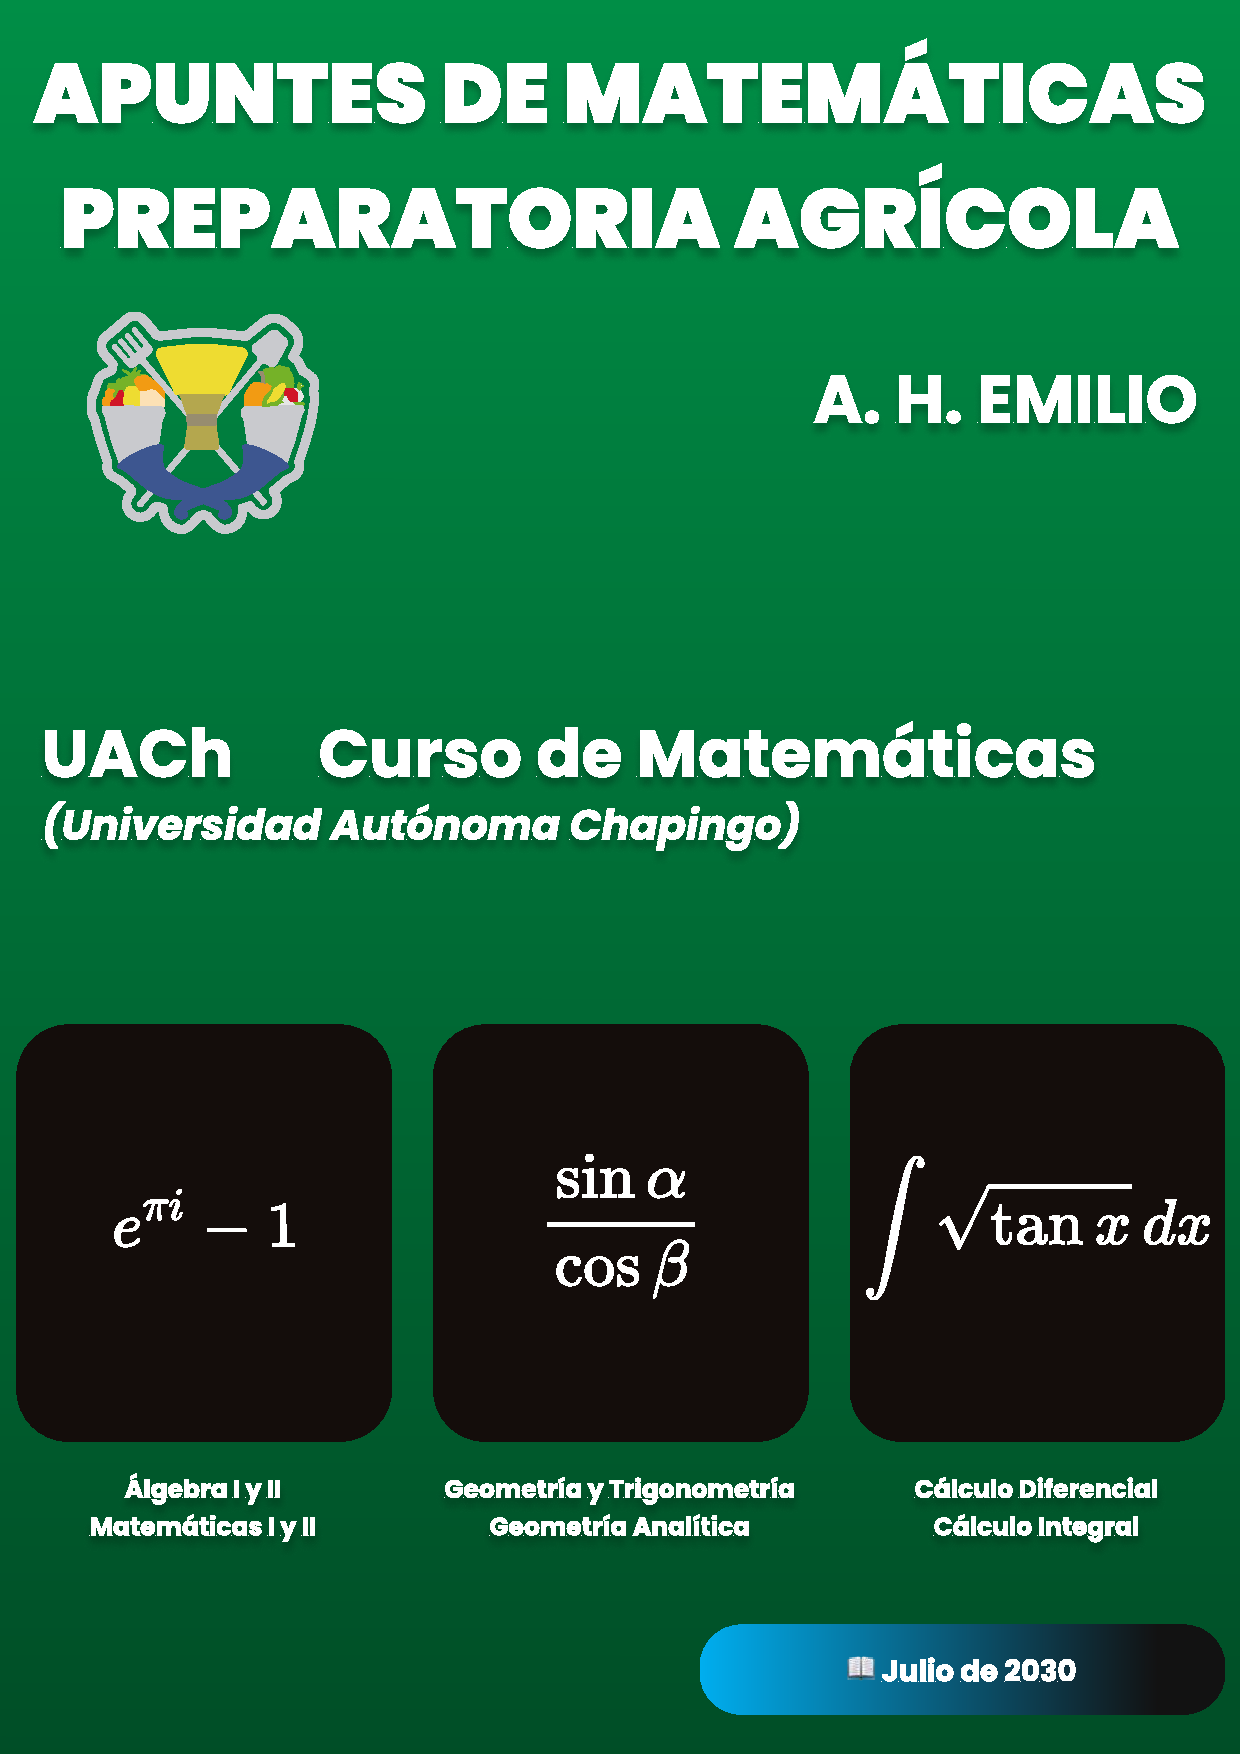
\includepdf[pages=1]{portada.pdf}
%----------------------------------------------------------------------------------------
%	COPYRIGHT PAGE
%----------------------------------------------------------------------------------------
\newpage
~\vfill
\thispagestyle{empty}

\noindent Copyright \copyright\ 2025 Emilio Álvarez Herrera\\ % Copyright notice

\noindent \textsc{Publicado por la Universidad Autónoma Chapingo}\\ % Publisher

\noindent \textsc{Página del autor} \url{https://emilio-ah.web.app}\\ 

\noindent Con licencia de Creative Commons Reconocimiento-No comercial 3.0 Unparted License (la `` Licencia ''). No puede utilizar este archivo excepto de conformidad con la Licencia. Puede obtener una copia de la licencia en \url {http://creativecommons.org/licenses/by-nc/3.0}. A menos que lo exija la ley aplicable o se acuerde por escrito, el software distribuido bajo la Licencia se distribuye en \textsc{`` tal cual '', sin garantías ni condiciones de ningún tipo}, ya sea expresa o implícita. Consulte la Licencia para conocer el idioma específico que rige los permisos y las limitaciones de la Licencia.\\ % License information

\noindent \textit{Primera edición, \today} % Printing/edition date (Noviembre del 2020)

%----------------------------------------------------------------------------------------
%	TABLE OF CONTENTS
%----------------------------------------------------------------------------------------

%\usechapterimagefalse % If you don't want to include a chapter image, use this to toggle images off - it can be enabled later with \usechapterimagetrue

%%%%%%%%%%%%%%%%%%%%%%%%%%%%%%%%%%%%%%%%%%%%%%%%%%%%%%%%%%%%%%%%%%%%%%%%%%%%%%%%%%%%%%%%%%%%%%%%%%%%%%%%%%%%%%%%%%%%%%%%%%%%%

\chapterimage{2.pdf} % Table of contents heading image

\pagestyle{empty} % No headers

\tableofcontents % Print the table of contents itself

\cleardoublepage % Forces the first chapter to start on an odd page so it's on the right

\pagestyle{fancy} % Print headers again
% ÉSTE ES EL LIBRO
%%%%%%%%%%%%%%%%%%%%%%%%%%%%%%%%%%%%%%%%%%%%%%%%%%%%%%%%%%%%%%%%%%%%%%%%%%%%%%
% \part{Primer semestre}
\chapterimage{1.pdf}
\chapter{Álgebra I}


\section{SISTEMAS NUMÉRICOS}% (3 semanas)
\subsection{Números Naturales, Enteros, Racionales, Irracionales, Reales y Primos.}
\subsection{Operaciones en los números: enteros y racionales.}
\subsection{Jerarquía de las operaciones y uso de símbolos de agrupación.}
\subsection{Problemas verbales con números racionales.}








\section{OPERATIVIDAD CON POLINOMIOS} %(3 semanas)
\subsection{Lenguaje común a lenguaje algebraico, primera parte.}
\subsection{Expresión y término algebraicos.}
\subsection{Términos semejantes.}
\subsection{Reducción de términos semejantes.}
\subsection{Eliminación de signos de agrupación.}
\subsection{Suma y resta de expresiones algebraicas.}
\subsection{Leyes de los exponentes para multiplicación y división de expresiones algebraicas.}
\subsection{Multiplicación de expresiones algebraicas.}
\subsection{División de expresiones algebraicas.}
\subsection{Lenguaje común a lenguaje algebraico, segunda parte.}
\subsection{Práctica 1. Operatividad con polinomios.}








\section{ECUACIONES DE PRIMER GRADO}% (3 semanas)

\subsection{Conceptos básicos}
\subsubsection{Ecuación}
\subsubsection{Propiedades de la igualdad.}
\subsection{Operaciones y procedimientos }
\subsubsection{Factorización por factor común.}
\subsubsection{Resolución de Ecuaciones de primer grado con una incógnita, con coeficientes enteros, fraccionarios, literales y despejes en formulas.}
\subsection{Problemas y aplicaciones}
\subsubsection{Plantear y resolver ecuaciones lineales a partir de problemas verbales.}


\section{FUNCIÓN LINEAL} % (3 semanas)
\subsection{Concepto general de función.}
\subsection{Variación directamente proporcional}
\subsection{Función Lineal}
\subsection{Tabular y graficar funciones lineales.}
\subsection{Aplicaciones y problemas.}
\subsection{Practica 2. Función lineal.}


\section{SISTEMAS DE ECUACIONES LINEALES}% (3 semanas)
\subsection{Conceptos básicos.}
\subsubsection{Sistema de ecuaciones.}
\subsubsection{Solución de un sistema de ecuaciones lineales.}
\subsubsection{Sistemas consistentes, inconsistentes y dependientes.}

\subsection{Operaciones y procedimientos.}

\subsubsection{Método de Igualación. (2x2 y 3x3)}
\subsubsection{Método de Sustitución. (2x2 y 3x3)}
\subsubsection{Método de Reducción (eliminación, sumas o restas). (2x2 y 3x3)}
\subsubsection{Método de Determinantes. (2x2 y 3x3)}

\subsection{Practica 3. Gráfica de sistema de ecuaciones lineales. (2x2)}

\subsection{Aplicaciones y problemas.}
\subsubsection{Plantear y resolver problemas.}
\subsubsection{Empleo de un sistema de ecuaciones lineales.}





\section{DESIGUALDAD LINEAL} % (1 semana)
\subsection{Conceptos}
\subsubsection{Concepto de intervalo.}
\subsubsection{Representar intervalos en la recta de los reales.}
\subsubsection{Desigualdad.}
\subsubsection{Propiedades de la desigualdad.}
\subsection{Operaciones y procedimientos}
\subsubsection{Resolver desigualdades lineales en forma gráfica y analítica.}


%%%%%%%%%%%%%%%%%%%%%%%%%%%%%%%%%%%%%%%%%%%%%%%%%%%%%%%%%%%%%%%%%%%%%%%%%%%%%%%%
% \part{Segundo semestre}
\chapterimage{2.pdf}
\chapter{Álgebra II}


\section{Función lineal} %(1.5 semanas)
\subsection{Concepto general de función.}
\subsection{Variación directamente proporcional}
\subsection{Función Lineal}
\subsection{Tabular y graficar funciones lineales.}








\section{Sistema de Ecuaciones lineales} %(4 semanas)
\subsection{Conceptos básicos.}
\subsubsection{Concepto de sistema de ecuaciones.}
\subsubsection{Concepto de solución de un sistema de ecuaciones lineales.}
\subsubsection{Concepto de solución consistente, inconsistente y dependiente.}
\subsection{Operaciones y procedimientos.}
\subsubsection{Métodos de solución de sistemas.}
\subsubsection{Igualación.}
\subsubsection{Sustitución.}
\subsubsection{Reducción (eliminación, sumas o restas).}
\subsubsection{Determinantes.}
\subsubsection{Gráfica de sistema de ecuaciones lineales de dos variables.}
\subsection{Aplicaciones y problemas.}
\subsubsection{Plantear y resolver problemas.}
\subsubsection{Empleo de un sistema de ecuaciones lineales.}







\section{Ecuaciones cuadráticas} %(3 semanas.)
\subsection{Ecuaciones cuadráticas y sus raíces o soluciones}
\subsection{La propiedad del producto cero y la resolución de ecuaciones por factorización.}
\subsection{Solución de ecuaciones cuadráticas completando el trinomio cuadrado perfecto.}
\subsection{Resolución de ecuaciones cuadráticas por la fórmula general.}
\subsection{El discriminante de una ecuación cuadrática y el tipo de raíces.}
\subsection{Solución de ecuaciones reducibles a cuadráticas, mediante un cambio de variable,}
\subsection{Resolución de ecuaciones que contienen radicales.}







\section{Funciones y desigualdades cuadráticas} %(4 semanas)
\subsection{Funciones cuadráticas.}
\subsection{Formas de representar una función cuadrática: tabular, gráfica y mediante una expresión algebraica}
\subsection{Elementos de una función cuadrática: intersección con los ejes coordenados; vértice de la parábola (máximo o mínimo), eje de simetría.}
\subsection{Transformaciones de la gráfica de y= x2}
\subsubsection{$y= (x+h)^2$}
\subsubsection{$y= ax^2$}
\subsubsection{$y=ax^2$}
\subsubsection{$y=x^2+k$}
\subsubsection{$y=a(x+h)^2+k$}
\subsection{Desigualdades cuadráticas.}
\subsection{Desigualdades lineales (un repaso)}
\subsection{Métodos para resolver una desigualdad cuadrática: Gráfico y Algebraico.}









\section{Sistema de ecuaciones cuadráticas} %(2 semanas)

\subsection{Ecuaciones cuadráticas de dos variables.}
\subsection{Gráficas de ecuaciones cuadráticas.}
\subsection{Métodos de resolución de sistemas cuadráticos}







\section{Expresiones exponenciales y logarítmicas} %(4 semanas)
\subsection{Exponentes racionales, función exponencial.}
\subsection{Logaritmos y funciones logarítmicas.}
\subsection{Propiedades de los logaritmos.}
\subsection{Logaritmos comunes y naturales.}
\subsection{Ecuaciones exponenciales y logarítmicas.}
\subsection{Problemas de crecimiento y decrecimiento.}

% %%%%%%%%%%%%%%%%%%%%%%%%%%%%%%%%%%%%%%%%%%%%%%%%%%%%%%%%%%%%%%%%%%%%%%%%%%%%%%%%
% \part{Tercer semestre}
\chapterimage{3.pdf}
\chapter{Geometría y Trigonometría} %( 3 horas)


\section{Conceptos básicos}

\subsection{Bosquejo histórico de la Geometría}
La geometría, una de las ramas más antiguas de las matemáticas, ha evolucionado a lo largo de los siglos, desde sus orígenes en la antigüedad hasta las formas más avanzadas de geometría moderna. Los antiguos egipcios y babilonios ya empleaban principios geométricos para resolver problemas prácticos, como la medición de tierras y la construcción de estructuras. Euclides, en su obra \emph{Los Elementos}, sistematizó gran parte del conocimiento geométrico de su tiempo, estableciendo axiomas y teoremas fundamentales que aún se estudian hoy en día. La geometría ha crecido para incluir no solo la geometría euclidiana clásica, sino también otras formas como la geometría no euclidiana, que exploran espacios curvos y multidimensionales.

\subsection{Términos no definidos}
En la geometría, ciertos conceptos se consideran primitivos o indefinibles porque no se explican mediante otros conceptos más básicos. Estos incluyen:
\begin{itemize}
    \item \textbf{Punto}: Una entidad sin dimensiones, que indica una posición en el espacio.
    \item \textbf{Línea (o recta)}: Una serie infinita de puntos que se extiende en ambas direcciones sin fin y sin ancho.
    \item \textbf{Plano}: Una superficie bidimensional que se extiende infinitamente en todas las direcciones.
\end{itemize}

\subsection{Postulados de la Recta}
Los postulados de la recta son afirmaciones aceptadas sin demostración que sirven como base para la geometría euclidiana. Algunos de los postulados de la recta incluyen:
\begin{enumerate}
    \item A través de dos puntos distintos pasa una única línea recta.
    \item Un segmento de línea puede prolongarse indefinidamente en ambas direcciones.
    \item Una línea recta puede dividir un plano en dos regiones distintas.
\end{enumerate}

\subsection{Axiomas de la Geometría}
Los axiomas de la geometría son proposiciones que se aceptan como verdaderas sin pruebas y que sirven como base para la deducción de otros teoremas. Algunos de los axiomas fundamentales incluyen:
\begin{enumerate}
    \item Los objetos iguales a un mismo objeto son iguales entre sí.
    \item Si se añaden cantidades iguales a cantidades iguales, los totales son iguales.
    \item Si se restan cantidades iguales de cantidades iguales, los restos son iguales.
\end{enumerate}

\subsection{Terminología y notación}
La terminología y notación en geometría son esenciales para una comunicación clara y precisa. Algunas notaciones comunes incluyen:
\begin{itemize}
    \item \textbf{Puntos}: Generalmente representados por letras mayúsculas (A, B, C, etc.).
    \item \textbf{Líneas}: Denotadas por letras minúsculas (l, m, n) o por dos puntos (AB).
    \item \textbf{Ángulos}: Representados por el símbolo $\angle$ seguido de tres letras, donde la letra del medio representa el vértice (ej. $\angle ABC$).
    \item \textbf{Segmentos de línea}: Denotados por dos puntos con una línea encima (ej. $\overline{AB}$).
    \item \textbf{Planos}: Representados por letras griegas (ej. plano $\alpha$, plano $\beta$).
\end{itemize}


\section{Ángulos} %(6 horas)

\subsection{Definición, clasificación de los ángulos}
Un ángulo es la figura formada por dos rayos que comparten un extremo común, llamado vértice del ángulo. Los ángulos se pueden clasificar de varias maneras:
\begin{itemize}
    \item \textbf{Ángulo agudo}: mide menos de 90°.
    \item \textbf{Ángulo recto}: mide exactamente 90°.
    \item \textbf{Ángulo obtuso}: mide más de 90° pero menos de 180°.
    \item \textbf{Ángulo llano}: mide exactamente 180°.
    \item \textbf{Ángulo completo}: mide 360°.
\end{itemize}

\subsection{Teorema de los ángulos opuestos por el vértice}
El teorema de los ángulos opuestos por el vértice establece que, cuando dos líneas se cruzan, los ángulos opuestos por el vértice son congruentes. Esto significa que tienen la misma medida.

\subsection{Ángulos que se forman entre parejas de rectas cortadas por una transversal}
Cuando una recta transversal corta dos rectas, se forman varios tipos de ángulos, incluyendo:
\begin{itemize}
    \item \textbf{Ángulos correspondientes}: Ángulos que están en el mismo lado de la transversal y en la misma posición relativa con respecto a las dos rectas.
    \item \textbf{Ángulos alternos internos}: Ángulos que están en lados opuestos de la transversal pero dentro de las dos rectas.
    \item \textbf{Ángulos alternos externos}: Ángulos que están en lados opuestos de la transversal pero fuera de las dos rectas.
    \item \textbf{Ángulos colaterales internos (suplementarios)}: Ángulos que están en el mismo lado de la transversal y entre las dos rectas.
\end{itemize}

\subsection{Problemas relativos a ángulos}
En esta sección se resolverán problemas aplicando los conceptos y teoremas discutidos.

 

\subsection{Terminología y notación}
La terminología y notación en geometría son esenciales para una comunicación clara y precisa. Algunas notaciones comunes incluyen:
\begin{itemize}
    \item \textbf{Puntos}: Generalmente representados por letras mayúsculas (A, B, C, etc.).
    \item \textbf{Líneas}: Denotadas por letras minúsculas (l, m, n) o por dos puntos (AB).
    \item \textbf{Ángulos}: Representados por el símbolo $\angle$ seguido de tres letras, donde la letra del medio representa el vértice (ej. $\angle ABC$).
    \item \textbf{Segmentos de línea}: Denotados por dos puntos con una línea encima (ej. $\overline{AB}$).
    \item \textbf{Planos}: Representados por letras griegas (ej. plano $\alpha$, plano $\beta$).
\end{itemize}




\section{Paralelismo y Perpendicularidad} % (6 horas)

\subsection{Definición: característica del paralelismo y la perpendicularidad}

En geometría, el \textbf{paralelismo} y la \textbf{perpendicularidad} son conceptos fundamentales que describen la relación entre dos o más líneas.

\subsubsection{Paralelismo}

Dos líneas son \textbf{paralelas} si y solo si nunca se intersectan y mantienen una distancia constante entre sí en todos sus puntos. Matemáticamente, se dice que dos líneas \( l_1 \) y \( l_2 \) son paralelas si la pendiente de \( l_1 \) es igual a la pendiente de \( l_2 \), en el caso de que ambas líneas estén expresadas en forma pendiente-intersección.

\begin{tikzpicture}
    \draw[thick] (0,0) -- (5,0) node[right] {$l_1$};
    \draw[thick] (0,1) -- (5,1) node[right] {$l_2$};
    \draw[dashed] (1,0) -- (1,1);
    \draw[dashed] (3,0) -- (3,1);
    \node at (0.5, -0.2) {D};
    \node at (2, -0.2) {D};
    \node at (4, -0.2) {D};
    \node[below] at (2.5, -0.2) {D};
\end{tikzpicture}

Donde \( D \) representa la distancia constante entre las dos líneas paralelas.

\subsubsection{Perpendicularidad}

Dos líneas son \textbf{perpendiculares} si se intersectan formando ángulos rectos, es decir, ángulos de \( 90^\circ \). Matemáticamente, si las pendientes de dos líneas \( m_1 \) y \( m_2 \) son tales que \( m_1 \cdot m_2 = -1 \), entonces las líneas son perpendiculares.

\begin{tikzpicture}
    \draw[thick] (0,0) -- (4,0) node[right] {$l_1$};
    \draw[thick] (2,-2) -- (2,2) node[above] {$l_2$};
    \draw[dashed] (2,0) -- (2,-1.5);
    \draw[dashed] (0,0) -- (2,-1.5);
    \draw[fill=black] (2,0) circle (2pt);
    \node at (2.3, 0.2) {90$^\circ$};
\end{tikzpicture}

Aquí, la intersección de las dos líneas forma un ángulo recto.

\subsection{Postulado del Paralelismo}

El \textbf{Postulado del Paralelismo} establece que dado un punto y una línea no contenida en el punto, existe una única línea que pasa por el punto y es paralela a la línea dada. Este postulado es uno de los axiomas fundamentales en la geometría euclidiana.

\subsection{Teorema Fundamental del Paralelismo}

Uno de los teoremas fundamentales del paralelismo es el \textbf{Teorema de la Alternancia de Ángulos}, que establece que si dos líneas paralelas son cortadas por una transversal, entonces los ángulos alternos internos son iguales.

\begin{tikzpicture}
    \draw[thick] (0,0) -- (4,0) node[right] {$l_1$};
    \draw[thick] (0,-2) -- (4,-2) node[right] {$l_2$};
    \draw[thick] (0,-2) -- (2,0);
    \draw[thick] (2,0) -- (4,-2);
    \node at (1.5, -1) {$\theta$};
    \node at (3.5, -1) {$\theta$};
    \node at (1, 0.3) {$\alpha$};
    \node at (3, 0.3) {$\alpha$};
\end{tikzpicture}

En el gráfico, los ángulos alternos internos \(\alpha\) y \(\theta\) son iguales.

\subsection{Problemas de Demostración}
% TODO
% \textbf{Problema 1:} Demuestra que si dos líneas son perpendiculares a una misma línea, entonces son paralelas entre sí.

% \textbf{Solución:} Sea \( l_1 \) y \( l_2 \) dos líneas perpendiculares a una línea \( l \). Como \( l_1 \) y \( l_2 \) son perpendiculares a \( l \), ambas forman ángulos rectos con \( l \). Así, los ángulos entre \( l_1 \) y \( l \) y entre \( l_2 \) y \( l \) son iguales, lo que implica que los ángulos entre \( l_1 \) y \( l_2 \) también son iguales. Por lo tanto, \( l_1 \) y \( l_2 \) son paralelas.

% \textbf{Problema 2:} Demuestra que la suma de los ángulos internos de un triángulo es igual a \( 180^\circ \) utilizando el concepto de paralelismo.

% \textbf{Solución:} Dibuja una línea paralela a uno de los lados del triángulo a través del vértice opuesto. Luego, usa el postulado del paralelismo para mostrar que los ángulos internos del triángulo se corresponden con los ángulos alternos internos y ángulos internos de la línea paralela. La suma de estos ángulos será \( 180^\circ \) debido a que forman una línea recta.


\section{Triángulos} % (4.5 horas)

El estudio de los triángulos es fundamental en geometría, ya que proporciona una base sólida para entender muchas propiedades geométricas. Esta sección se enfoca en la definición, clasificación y propiedades de los triángulos, así como en las rectas y puntos notables.

\subsection{Definición y Clasificación de los Triángulos}

Un \textbf{triángulo} es una figura geométrica formada por tres segmentos de línea que se encuentran en tres puntos no colineales, llamados \textbf{vértices}. Los segmentos de línea son los \textbf{lados} del triángulo.

\subsubsection{Clasificación según los Ángulos}

Los triángulos se clasifican en función de sus ángulos internos:

\begin{itemize}
    \item \textbf{Triángulo Acutángulo:} Todos sus ángulos son menores a \( 90^\circ \).
    \item \textbf{Triángulo Rectángulo:} Tiene un ángulo de \( 90^\circ \).
    \item \textbf{Triángulo Obtusángulo:} Tiene un ángulo mayor a \( 90^\circ \).
\end{itemize}

\begin{tikzpicture}
    \draw[thick] (0,0) -- (3,0) -- (1.5,2) -- cycle;
    \node at (1.5, 0.2) {Acutangulo};
    \draw[thick] (5,0) -- (8,0) -- (6.5,2) -- cycle;
    \node at (6.5, 0.2) {Rectangulo};
    \draw[thick] (10,0) -- (13,0) -- (11.5,2) -- cycle;
    \node at (11.5, 0.2) {Obtusangulo};
\end{tikzpicture}

\subsubsection{Clasificación según los Lados}

Los triángulos también se clasifican según la longitud de sus lados:

\begin{itemize}
    \item \textbf{Triángulo Equilátero:} Todos sus lados son de igual longitud.
    \item \textbf{Triángulo Isósceles:} Tiene dos lados de igual longitud.
    \item \textbf{Triángulo Escaleno:} Todos sus lados son de diferente longitud.
\end{itemize}

\begin{tikzpicture}
    \draw[thick] (0,0) -- (2,0) -- (1,1.7) -- cycle;
    \node at (1, -0.3) {Equilatero};
    \draw[thick] (4,0) -- (6,0) -- (5,1.7) -- cycle;
    \node at (5, -0.3) {Isosceles};
    \draw[thick] (8,0) -- (10,0) -- (9,1.7) -- cycle;
    \node at (9, -0.3) {Escaleno};
\end{tikzpicture}

\subsection{Teorema de los Ángulos Interiores de un Triángulo}

El \textbf{Teorema de los Ángulos Interiores} establece que la suma de los ángulos internos de un triángulo es siempre igual a \( 180^\circ \).

\begin{tikzpicture}
    \draw[thick] (0,0) -- (4,0) -- (2,3) -- cycle;
    \node at (0.5, -0.2) {$\alpha$};
    \node at (3.5, -0.2) {$\beta$};
    \node at (2, 3.2) {$\gamma$};
    \draw[dashed] (2,0) -- (2,3);
    \draw[dashed] (0,0) -- (2,3);
    \draw[dashed] (4,0) -- (2,3);
    \node at (2, -0.5) {Suma = 180$^\circ$};
\end{tikzpicture}

\subsection{Rectas y Puntos Notables de los Triángulos}

Los triángulos tienen varios puntos y rectas notables que son importantes para resolver problemas geométricos.

\subsubsection{Puntos Notables}

\begin{itemize}
    \item \textbf{Baricentro:} Punto de concurrencia de las medianas del triángulo.
    \item \textbf{Ortocentro:} Punto de concurrencia de las alturas del triángulo.
    \item \textbf{Circuncentro:} Punto de concurrencia de las mediatrices de los lados del triángulo.
    \item \textbf{Incentro:} Punto de concurrencia de las bisectrices de los ángulos del triángulo.
\end{itemize}

\subsubsection{Rectas Notables}

\begin{itemize}
    \item \textbf{Mediana:} Segmento que une un vértice con el punto medio del lado opuesto.
    \item \textbf{Altura:} Segmento perpendicular desde un vértice al lado opuesto.
    \item \textbf{Mediatriz:} Recta perpendicular a un lado del triángulo que pasa por su punto medio.
    \item \textbf{Bisectriz:} Recta que divide un ángulo en dos ángulos iguales.
\end{itemize}

\begin{tikzpicture}
    \draw[thick] (0,0) -- (4,0) -- (2,3) -- cycle;
    \draw[dashed] (2,0) -- (2,3); % Altura
    \draw[dashed] (0,0) -- (2,1.5); % Mediana
    \draw[dashed] (4,0) -- (2,1.5); % Mediana
    \draw[fill=black] (2,1.5) circle (2pt); % Circuncentro
    \node at (2, -0.2) {Altura};
    \node at (2.5, 2.2) {Mediana};
    \node at (1.5, 1.5) {Circuncentro};
\end{tikzpicture}


\section{Congruencia} % (6 horas)

\subsection{Concepto de Congruencia}

Dos figuras geométricas son \textbf{congruentes} si tienen la misma forma y tamaño. Esto significa que se pueden superponer una sobre otra mediante una secuencia de transformaciones geométricas: traslaciones, rotaciones y reflexiones. En particular, dos triángulos son congruentes si sus ángulos y lados correspondientes son iguales.

\begin{center}
\begin{tikzpicture}
    % Triángulo 1
    \draw[thick] (0,0) -- (4,0) -- (2,3) -- cycle;
    \node at (0,0) [below left] {A};
    \node at (4,0) [below right] {B};
    \node at (2,3) [above] {C};
    
    % Triángulo 2
    \draw[thick] (6,0) -- (10,0) -- (8,3) -- cycle;
    \node at (6,0) [below left] {D};
    \node at (10,0) [below right] {E};
    \node at (8,3) [above] {F};
    
    \node at (2, -1) {Triángulo $ABC$};
    \node at (8, -1) {Triángulo $DEF$};
    
    % Líneas de congruencia
    \draw[dashed] (0,0) -- (6,0);
    \draw[dashed] (4,0) -- (10,0);
    \draw[dashed] (2,3) -- (8,3);
    
    % Etiquetas de ángulos
    \node at (0.5, 0.3) {$\alpha$};
    \node at (4.5, 0.3) {$\alpha$};
    \node at (2, 2.7) {$\beta$};
    \node at (8, 2.7) {$\beta$};
    \node at (1.5, 1) {$\gamma$};
    \node at (7.5, 1) {$\gamma$};
\end{tikzpicture}
\end{center}

En la figura anterior, los triángulos $ABC$ y $DEF$ son congruentes porque sus ángulos y lados correspondientes son iguales.

\subsection{Postulados de Congruencia}

Para determinar si dos triángulos son congruentes, se utilizan los siguientes postulados:

\begin{itemize}
    \item \textbf{Postulado Lado-Lado-Lado (LLL):} Si en dos triángulos, los tres lados de uno son iguales a los tres lados del otro, entonces los triángulos son congruentes.
    \item \textbf{Postulado Ángulo-Lado-Ángulo (ALA):} Si en dos triángulos, un ángulo y los dos lados adyacentes a ese ángulo son iguales a los correspondientes en otro triángulo, entonces los triángulos son congruentes.
    \item \textbf{Postulado Ángulo-Ángulo-Lado (AAL):} Si en dos triángulos, dos ángulos y el lado no comprendido entre ellos son iguales a los correspondientes en otro triángulo, entonces los triángulos son congruentes.
\end{itemize}

\subsection{Teorema del Triángulo Isósceles}

Un triángulo es \textbf{isósceles} si tiene al menos dos lados iguales. El teorema del triángulo isósceles establece que:

\begin{itemize}
    \item Los ángulos opuestos a los lados iguales son también iguales.
    \item La altura, mediana y bisectriz desde el vértice del ángulo de los dos lados iguales son coincidentes.
\end{itemize}

\begin{center}
\begin{tikzpicture}
    % Triángulo Isósceles
    \draw[thick] (0,0) -- (4,0) -- (2,3) -- cycle;
    \node at (0,0) [below left] {A};
    \node at (4,0) [below right] {B};
    \node at (2,3) [above] {C};
    \draw[dashed] (2,0) -- (2,3);
    
    % Ángulos
    \node at (1, -0.3) {a};
    \node at (3, -0.3) {a};
    \node at (2.5, 2) {b};
    \node at (1.5, 2) {b};
    
    % Líneas
    \draw[dashed] (0,0) -- (2,3);
    \draw[dashed] (4,0) -- (2,3);
    \node at (2, -1) {Triángulo Isósceles $ABC$};
\end{tikzpicture}
\end{center}

\subsection{Problemas de Aplicación}

% \begin{enumerate}
%     \item Dado un triángulo con lados $AB = AC$ y ángulos $\angle ABC = \angle ACB$, demuestra que el triángulo es isósceles.
%     \item Usando los postulados de congruencia, demuestra que los triángulos formados al cortar un triángulo rectángulo por su mediana son congruentes.
%     \item Resuelve el siguiente problema: En un triángulo $XYZ$, si $XY = YZ$ y $\angle X = \angle Z$, ¿cómo se puede demostrar que el triángulo es isósceles?
% \end{enumerate}










\section{Semejanza} %(10.5 horas)

\subsection{Razones y Proporciones}

\begin{definition}
    \textbf{Razón:} Una razón es la relación entre dos magnitudes de la misma especie, expresada como una fracción o un cociente. 
\end{definition}

\begin{definition}
    \textbf{Proporción:} Una proporción es una igualdad entre dos razones. Se expresa como \(\frac{a}{b} = \frac{c}{d}\), donde \(a\), \(b\), \(c\) y \(d\) son magnitudes positivas.
\end{definition}

\begin{example}
    Consideremos las razones \(\frac{2}{3}\) y \(\frac{4}{6}\). Como \(\frac{2}{3} = \frac{4}{6}\), decimos que estas razones son proporcionales.
\end{example}

\subsection{Concepto de Semejanza. Triángulos Semejantes}

\begin{definition}
    \textbf{Semejanza de Triángulos:} Dos triángulos son semejantes si tienen sus ángulos correspondientes iguales y sus lados correspondientes proporcionales.
\end{definition}

\begin{example}
    Dos triángulos con ángulos iguales y lados proporcionales se llaman triángulos semejantes. Por ejemplo, si \(\triangle ABC \sim \triangle DEF\), entonces \(\frac{AB}{DE} = \frac{BC}{EF} = \frac{CA}{FD}\).
\end{example}

\subsection{Postulado de Semejanza}

\begin{definition}
    Los postulados de semejanza para triángulos son:
    \begin{itemize}
        \item \textbf{Postulado AAA:} Si dos triángulos tienen sus ángulos correspondientes iguales, entonces son semejantes.
        \item \textbf{Postulado LAL:} Si un ángulo y los dos lados adyacentes de un triángulo son proporcionales a un ángulo y los dos lados adyacentes de otro triángulo, entonces los triángulos son semejantes.
        \item \textbf{Postulado LLL:} Si los tres lados de un triángulo son proporcionales a los tres lados de otro triángulo, entonces los triángulos son semejantes.
    \end{itemize}
\end{definition}

\begin{tikzpicture}
    % Triángulo AAA
    \draw[thick] (0,0) -- (4,0) -- (2,3) -- cycle;
    \node at (0,0) [below left] {A};
    \node at (4,0) [below right] {B};
    \node at (2,3) [above] {C};
    \node at (2, -1) {Triángulo $ABC$};
    
    % Triángulo similar AAA
    \draw[thick] (6,0) -- (10,0) -- (8,3) -- cycle;
    \node at (6,0) [below left] {D};
    \node at (10,0) [below right] {E};
    \node at (8,3) [above] {F};
    \node at (8, -1) {Triángulo $DEF$};
    
    % Líneas de semejanza
    \draw[dashed] (0,0) -- (6,0);
    \draw[dashed] (4,0) -- (10,0);
    \draw[dashed] (2,3) -- (8,3);
    
    % Etiquetas de ángulos
    \node at (0.5, 0.5) {$\alpha$};
    \node at (6.5, 0.5) {$\alpha$};
    \node at (3.5, 2) {$\beta$};
    \node at (9.5, 2) {$\beta$};
    \node at (2, 0.5) {$a$};
    \node at (8, 0.5) {$a$};
\end{tikzpicture}

\subsection{Teorema de Pitágoras}

\begin{theorem}[Teorema de Pitágoras]
    En un triángulo rectángulo, el cuadrado de la hipotenusa es igual a la suma de los cuadrados de los catetos. Es decir, si \(a\) y \(b\) son los catetos y \(c\) es la hipotenusa, entonces \(c^2 = a^2 + b^2\).
\end{theorem}

\begin{tikzpicture}
    % Triángulo Rectángulo
    \draw[thick] (0,0) -- (4,0) -- (0,3) -- cycle;
    \node at (0,0) [below left] {A};
    \node at (4,0) [below right] {B};
    \node at (0,3) [above left] {C};
    
    % Etiquetas de lados
    \node at (2, -0.5) {$a$};
    \node at (-0.5, 1.5) {$b$};
    \node at (2, 1.5) {$c$};
    
    % Ángulo recto
    \node at (0.3, 0.3) {$90^\circ$};
\end{tikzpicture}

\subsection{Teorema Fundamental de Proporcionalidad}

\begin{theorem}[Teorema Fundamental de Proporcionalidad]
    Si se traza una recta paralela a uno de los lados de un triángulo, entonces se forma un triángulo semejante al triángulo dado, y los segmentos de los otros dos lados son proporcionales.
\end{theorem}

\begin{tikzpicture}
    % Triángulo y recta paralela
    \draw[thick] (0,0) -- (5,0) -- (2,4) -- cycle;
    \draw[dashed] (2,4) -- (5,0);
    \draw[dashed] (2,4) -- (0,0);
    \draw[dashed] (2,2.5) -- (5,2.5);
    
    % Etiquetas
    \node at (0,0) [below left] {A};
    \node at (5,0) [below right] {B};
    \node at (2,4) [above] {C};
    \node at (2,2.5) [below] {D};
    \node at (5,2.5) [right] {E};
    
    % Etiquetas de proporciones
    \node at (2.5, 0.3) {$\frac{AD}{DB}$};
    \node at (3.7, 3) {$\frac{CE}{EC}$};
\end{tikzpicture}


\section{Funciones Trigonométricas} %(7.5 horas)

\subsection{Introducción a la Trigonometría}

\begin{definition}
    \textbf{Trigonometría:} La trigonometría es la rama de las matemáticas que estudia las relaciones entre los ángulos y los lados de los triángulos. Su desarrollo histórico se remonta a las civilizaciones antiguas como los egipcios y babilonios, y fue formalmente desarrollada por los griegos y los indios en la antigüedad.
\end{definition}

\begin{itemize}
    \item \textbf{Breve semblanza histórica:} La trigonometría tiene sus raíces en la astronomía y la geometría. Los antiguos griegos, como Hiparco y Ptolomeo, hicieron contribuciones significativas, y la trigonometría se desarrolló aún más en la India y el mundo islámico durante la Edad Media.
    \item \textbf{Importancia para el Ingeniero Agrónomo:} La trigonometría es crucial para medir distancias inaccesibles y resolver problemas relacionados con la topografía y la geometría del terreno.
    \item \textbf{Objetivo general del curso:} Proporcionar una comprensión sólida de las funciones trigonométricas y su aplicación en la resolución de triángulos rectángulos.
    \item \textbf{Ubicación en el plan de estudios:} La trigonometría se ubica en el estudio de las matemáticas aplicadas, y es fundamental para la ingeniería y las ciencias aplicadas.
\end{itemize}

\subsection{Funciones Trigonométricas de un Ángulo Agudo de un Triángulo Rectángulo}

\begin{definition}
    \textbf{Funciones Trigonométricas:} Para un ángulo agudo en un triángulo rectángulo, las funciones trigonométricas principales son:
    \begin{itemize}
        \item \textbf{Seno} (\(\sin\)): \(\sin(\theta) = \frac{\text{lado opuesto}}{\text{hipotenusa}}\)
        \item \textbf{Coseno} (\(\cos\)): \(\cos(\theta) = \frac{\text{lado adyacente}}{\text{hipotenusa}}\)
        \item \textbf{Tangente} (\(\tan\)): \(\tan(\theta) = \frac{\text{lado opuesto}}{\text{lado adyacente}}\)
    \end{itemize}
\end{definition}

\begin{example}
    En un triángulo rectángulo con un ángulo de \(30^\circ\), si la hipotenusa es 10 unidades, entonces:
    \[
    \sin(30^\circ) = \frac{1}{2} \quad \text{y} \quad \text{lado opuesto} = 10 \times \frac{1}{2} = 5
    \]
\end{example}

\subsection{Manejo de Tablas y/o Calculadora}

\begin{definition}
    \textbf{Tablas y Calculadora:} Las tablas trigonométricas y las calculadoras permiten encontrar los valores de las funciones trigonométricas para ángulos dados. Es fundamental familiarizarse con su uso para resolver problemas de trigonometría de manera eficiente.
\end{definition}

\begin{example}
    Para encontrar \(\sin(45^\circ)\) usando una calculadora:
    \[
    \sin(45^\circ) \approx 0.707
    \]
\end{example}

\subsection{Triángulos Especiales}

\begin{definition}
    \textbf{Triángulos Especiales:} Existen triángulos rectángulos especiales que tienen ángulos de \(30^\circ\), \(45^\circ\) y \(60^\circ\). Estos triángulos tienen propiedades y razones trigonométricas específicas:
    \begin{itemize}
        \item Triángulo \(30^\circ-60^\circ-90^\circ\): Las longitudes de los lados están en la proporción 1 : \(\sqrt{3}\) : 2.
        \item Triángulo \(45^\circ-45^\circ-90^\circ\): Las longitudes de los lados están en la proporción 1 : 1 : \(\sqrt{2}\).
    \end{itemize}
\end{definition}

\begin{tikzpicture}
    % Triángulo 30-60-90
    \draw[thick] (0,0) -- (6,0) -- (0,3) -- cycle;
    \node at (0,0) [below left] {A};
    \node at (6,0) [below right] {B};
    \node at (0,3) [above left] {C};
    
    % Etiquetas
    \node at (3, -0.5) {$2x$};
    \node at (-0.5, 1.5) {$x$};
    \node at (3, 1.5) {$x\sqrt{3}$};
    
    % Ángulos
    \node at (0.5, 0.5) {$30^\circ$};
    \node at (5.5, 0.5) {$60^\circ$};
    \node at (0.5, 2.5) {$90^\circ$};
\end{tikzpicture}

\subsection{Solución de Triángulos Rectángulos, Cálculo de Áreas}

\begin{definition}
    \textbf{Solución de Triángulos Rectángulos:} Consiste en encontrar las longitudes de los lados y los ángulos de un triángulo rectángulo utilizando funciones trigonométricas. El área de un triángulo rectángulo se calcula como:
    \[
    \text{Área} = \frac{1}{2} \times \text{base} \times \text{altura}
    \]
\end{definition}

\begin{example}
    En un triángulo rectángulo con base 6 y altura 8, el área es:
    \[
    \text{Área} = \frac{1}{2} \times 6 \times 8 = 24
    \]
\end{example}

\subsection{Ángulos de Elevación y Depresión}

\begin{definition}
    \textbf{Ángulos de Elevación y Depresión:} El ángulo de elevación es el ángulo formado por la línea de visión hacia arriba desde un punto de observación. El ángulo de depresión es el ángulo formado por la línea de visión hacia abajo desde un punto de observación. Ambos se utilizan para resolver problemas de altura y distancia.
\end{definition}

\begin{tikzpicture}
    % Ángulo de elevación y depresión
    \draw[thick] (0,0) -- (5,0) -- (5,4) -- cycle;
    \draw[dashed] (0,0) -- (5,4);
    \draw[dashed] (5,0) -- (5,2);
    
    % Etiquetas
    \node at (0,0) [below left] {A};
    \node at (5,0) [below right] {B};
    \node at (5,4) [above right] {C};
    \node at (5,2) [right] {D};
    
    % Ángulos
    \node at (2.5, -0.5) {$\text{Distancia}$};
    \node at (5.5, 2) {$\text{Ángulo de Elevación}$};
    \node at (2.5, 4.5) {$\text{Ángulo de Depresión}$};
\end{tikzpicture}


\section{Funciones Trigonométricas} %(7.5 horas)

\subsection{Sistema de Coordenadas Rectangulares}

\begin{definition}
    \textbf{Sistema de Coordenadas Rectangulares:} El sistema de coordenadas rectangulares, también conocido como sistema de coordenadas cartesianas, está formado por dos ejes perpendiculares: el eje \(x\) (horizontal) y el eje \(y\) (vertical). Cada punto en el plano se localiza mediante un par de coordenadas \((x, y)\), donde \(x\) es la distancia desde el eje \(y\) y \(y\) es la distancia desde el eje \(x\).
\end{definition}

\subsection{Definir Grados y Radianes, Conversiones de un Sistema al Otro}

\begin{definition}
    \textbf{Grados y Radianes:} 
    \begin{itemize}
        \item \textbf{Grados:} Un círculo completo tiene 360 grados.
        \item \textbf{Radianes:} Un círculo completo tiene \(2\pi\) radianes. La conversión entre grados y radianes se realiza mediante las siguientes fórmulas:
        \[
        \text{Radianes} = \text{Grados} \times \frac{\pi}{180}
        \]
        \[
        \text{Grados} = \text{Radianes} \times \frac{180}{\pi}
        \]
    \end{itemize}
\end{definition}

\begin{example}
    Convertir \(45^\circ\) a radianes:
    \[
    45^\circ \times \frac{\pi}{180} = \frac{\pi}{4}
    \]
\end{example}

\subsection{Ángulo en Posición Normal, Concepto de Ángulo Reducido o de Referencia}

\begin{definition}
    \textbf{Ángulo en Posición Normal:} Un ángulo está en posición normal cuando su vértice está en el origen y uno de sus lados está en el eje positivo \(x\). Los ángulos se miden en sentido antihorario desde el eje positivo \(x\).
    
    \textbf{Ángulo Reducido o de Referencia:} Es el ángulo agudo formado entre el lado terminal del ángulo en posición normal y el eje \(x\).
\end{definition}

\begin{example}
    Para un ángulo de \(135^\circ\), el ángulo de referencia es \(180^\circ - 135^\circ = 45^\circ\).
\end{example}

\subsection{Definición de las Funciones Trigonométricas de un Ángulo Cualquiera en Posición Normal}

\begin{definition}
    \textbf{Funciones Trigonométricas en Posición Normal:} 
    \begin{itemize}
        \item \textbf{Seno} (\(\sin\)): La razón del lado opuesto al ángulo dividido por la hipotenusa.
        \item \textbf{Coseno} (\(\cos\)): La razón del lado adyacente al ángulo dividido por la hipotenusa.
        \item \textbf{Tangente} (\(\tan\)): La razón del seno sobre el coseno.
    \end{itemize}
\end{definition}

\begin{example}
    Para un ángulo de \(150^\circ\) (en el segundo cuadrante), el seno es positivo y el coseno es negativo. El ángulo de referencia es \(30^\circ\):
    \[
    \sin(150^\circ) = \sin(30^\circ) = \frac{1}{2}
    \]
    \[
    \cos(150^\circ) = -\cos(30^\circ) = -\frac{\sqrt{3}}{2}
    \]
\end{example}

\subsection{Signo de las Funciones Trigonométricas en los Cuatro Cuadrantes}

\begin{definition}
    \textbf{Signo de las Funciones Trigonométricas:} 
    \begin{itemize}
        \item \textbf{Primer Cuadrante} (\(0^\circ\) a \(90^\circ\)): \(\sin\), \(\cos\), y \(\tan\) son positivos.
        \item \textbf{Segundo Cuadrante} (\(90^\circ\) a \(180^\circ\)): \(\sin\) es positivo, \(\cos\) y \(\tan\) son negativos.
        \item \textbf{Tercer Cuadrante} (\(180^\circ\) a \(270^\circ\)): \(\tan\) es positivo, \(\sin\) y \(\cos\) son negativos.
        \item \textbf{Cuarto Cuadrante} (\(270^\circ\) a \(360^\circ\)): \(\cos\) es positivo, \(\sin\) y \(\tan\) son negativos.
    \end{itemize}
\end{definition}

\subsection{Ángulos Positivos, Ángulos Negativos}

\begin{definition}
    \textbf{Ángulos Positivos y Negativos:} 
    \begin{itemize}
        \item \textbf{Ángulos Positivos:} Se miden en sentido antihorario desde el eje \(x\).
        \item \textbf{Ángulos Negativos:} Se miden en sentido horario desde el eje \(x\).
    \end{itemize}
\end{definition}

\begin{example}
    Un ángulo de \(-30^\circ\) es equivalente a \(360^\circ - 30^\circ = 330^\circ\).
\end{example}

\subsection{Funciones Trigonométricas Inversas}

\begin{definition}
    \textbf{Funciones Trigonométricas Inversas:} Las funciones trigonométricas inversas son:
    \begin{itemize}
        \item \textbf{Arco seno} (\(\sin^{-1}\)): Determina el ángulo cuyo seno es el valor dado.
        \item \textbf{Arco coseno} (\(\cos^{-1}\)): Determina el ángulo cuyo coseno es el valor dado.
        \item \textbf{Arco tangente} (\(\tan^{-1}\)): Determina el ángulo cuyo tangente es el valor dado.
    \end{itemize}
\end{definition}

\begin{example}
    Para encontrar el ángulo cuyo seno es \(\frac{1}{2}\):
    \[
    \sin^{-1}\left(\frac{1}{2}\right) = 30^\circ
    \]
\end{example}


\section{Círculo Trigonométrico, Graficación de las Funciones Trigonométricas} %(4.5 horas)

\subsection{El Círculo Trigonométrico}

\begin{definition}
    \textbf{Círculo Trigonométrico:} Es un círculo con radio 1 centrado en el origen del sistema de coordenadas cartesianas. Los puntos en el círculo corresponden a los valores de las funciones trigonométricas de un ángulo.
\end{definition}

\begin{tikzpicture}
    % Draw the axes
    \draw[->] (-2.5,0) -- (2.5,0) node[right] {$x$};
    \draw[->] (0,-2.5) -- (0,2.5) node[above] {$y$};
    
    % Draw the unit circle
    \draw[thick] (0,0) circle(2);
    
    % Draw the angle
    \draw[thick, ->] (0,0) -- (1.5,1.5) coordinate (A) node[midway, above right]{};
    
    % Draw the radius line to the circle
    \draw[dashed] (0,0) -- (2,0) node[below right] {1};
    \draw[dashed] (0,0) -- (0,2) node[above left] {1};
    
    % Draw the cosine line
    \draw[thick, blue, ->] (0,0) -- (1.5,0) node[below] {$\cos\theta$};
    
    % Draw the sine line
    \draw[thick, red, ->] (0,0) -- (0,1.5) node[left] {$\sin\theta$};
    
    % Draw the tangent line
    % \draw[thick, green, ->] (1.5,0) -- (1.5,1.5) node[right] {$\tan\theta$};
    
    % Label the angle
    \node at (1.8, 0.3) {$(\cos\theta, \sin\theta)$};
    
    % Draw dashed lines
    \draw[dashed] (1.5,0) -- (1.5,1.5);
    \draw[dashed] (0,1.5) -- (1.5,1.5);
    
    % Draw the origin label
    \node at (0,0) [below left] {O};
    
    % Draw the angle label
    \node at (0.7, 0.3) {$\theta$};
\end{tikzpicture}

\subsection{Funciones Trigonométricas Definidas como Segmentos Rectilíneos}

\begin{definition}
    \textbf{Funciones Trigonométricas como Segmentos Rectilíneos:} Las funciones trigonométricas pueden ser representadas como segmentos rectilíneos en el círculo trigonométrico:
    \begin{itemize}
        \item \textbf{Seno} (\(\sin\theta\)): La coordenada \(y\) del punto en el círculo.
        \item \textbf{Coseno} (\(\cos\theta\)): La coordenada \(x\) del punto en el círculo.
        \item \textbf{Tangente} (\(\tan\theta\)): La razón de \(\sin\theta\) sobre \(\cos\theta\).
    \end{itemize}
\end{definition}

\begin{example}
    Para \(\theta = 45^\circ\):
    \[
    \sin 45^\circ = \frac{\sqrt{2}}{2}
    \]
    \[
    \cos 45^\circ = \frac{\sqrt{2}}{2}
    \]
    \[
    \tan 45^\circ = 1
    \]
\end{example}

\subsection{Variaciones de las Funciones Trigonométricas con Respecto a la Variación del Argumento en los Cuatro Cuadrantes}

\begin{definition}
    \textbf{Variaciones en los Cuadrantes:}
    \begin{itemize}
        \item \textbf{Primer Cuadrante} (\(0^\circ\) a \(90^\circ\)): \(\sin\) y \(\cos\) son positivos.
        \item \textbf{Segundo Cuadrante} (\(90^\circ\) a \(180^\circ\)): \(\sin\) es positivo, \(\cos\) es negativo.
        \item \textbf{Tercer Cuadrante} (\(180^\circ\) a \(270^\circ\)): \(\sin\) y \(\cos\) son negativos.
        \item \textbf{Cuarto Cuadrante} (\(270^\circ\) a \(360^\circ\)): \(\sin\) es negativo, \(\cos\) es positivo.
    \end{itemize}
\end{definition}

\begin{example}
    Para un ángulo de \(210^\circ\) en el tercer cuadrante:
    \[
    \sin 210^\circ = -\frac{1}{2}
    \]
    \[
    \cos 210^\circ = -\frac{\sqrt{3}}{2}
    \]
\end{example}

\subsection{Graficación de las Funciones Trigonométricas}

\begin{definition}
    \textbf{Graficación de Funciones Trigonométricas:}
    \begin{itemize}
        \item \textbf{Seno y Coseno:} Tienen una gráfica periódica con periodo \(2\pi\). La gráfica de \(\sin x\) y \(\cos x\) es una onda que oscila entre \(-1\) y \(1\).
        \item \textbf{Tangente:} Tiene una gráfica con asíntotas verticales en los puntos donde \(\cos x = 0\) y oscila entre \(-\infty\) y \(\infty\).
    \end{itemize}
\end{definition}

\begin{example}
    La gráfica de \(\sin x\) tiene un periodo de \(2\pi\) y oscila entre \(-1\) y \(1\). La gráfica de \(\sin x\) puede ser representada por:
    \[
    y = a \sin(bx + c) + d
    \]
    donde \(a\) es la amplitud, \(b\) afecta el periodo, \(c\) es el desfase horizontal, y \(d\) es el desfase vertical.
\end{example}

\begin{tikzpicture}
    \draw[->] (-1,0) -- (7,0) node[right] {$x$};
    \draw[->] (0,-1.5) -- (0,1.5) node[above] {$y$};
    
    % Función seno
    \draw[blue,thick,->] plot[domain=0:6.5,samples=100] (\x,{sin(\x r)}) node[right] {$\sin x$};
    \draw[dashed] (3.14,-1.5) -- (3.14,1.5);
    \draw[dashed] (6.28,-1.5) -- (6.28,1.5);
\end{tikzpicture}




\section{Triángulos oblicuángulos} %(6 horas)

\subsection{Ley de Senos y Cosenos}

Para abordar la resolución de triángulos oblicuángulos, es fundamental conocer y aplicar la Ley de Senos y la Ley de Cosenos. Estas leyes nos permiten determinar las medidas de los ángulos y los lados de un triángulo cuando se dispone de ciertos datos. La Ley de Senos establece que, en cualquier triángulo, la razón entre un lado y el seno del ángulo opuesto es constante. Matemáticamente, se expresa como:

\[
\frac{a}{\sin A} = \frac{b}{\sin B} = \frac{c}{\sin C}
\]

donde \(a\), \(b\) y \(c\) son los lados del triángulo, y \(A\), \(B\) y \(C\) son los ángulos opuestos. Esta ley es especialmente útil cuando se conocen dos ángulos y un lado, o dos lados y un ángulo no comprendido.

Por otro lado, la Ley de Cosenos generaliza el teorema de Pitágoras para triángulos que no son rectángulos. Se utiliza para encontrar un lado de un triángulo cuando se conocen los otros dos lados y el ángulo comprendido, o para encontrar el ángulo cuando se conocen los tres lados. Se expresa como:

\[
c^2 = a^2 + b^2 - 2ab \cos C
\]

donde \(c\) es el lado opuesto al ángulo \(C\), y \(a\) y \(b\) son los otros dos lados. Esta ley es crucial para resolver triángulos oblicuángulos cuando se dispone de información diferente de la proporcionada por la Ley de Senos.

\subsection{Solución de Triángulos Oblicuángulos}

Para resolver un triángulo oblicuángulo, es necesario aplicar la Ley de Senos y la Ley de Cosenos de manera adecuada según los datos disponibles. Por ejemplo, si se conocen dos ángulos y un lado, la Ley de Senos permite calcular los lados restantes y el tercer ángulo utilizando la propiedad de que la suma de los ángulos en un triángulo es \(180^\circ\). En cambio, si se conocen dos lados y el ángulo comprendido, se puede usar la Ley de Cosenos para encontrar el tercer lado y, posteriormente, aplicar la Ley de Senos para determinar los ángulos restantes.

Para ilustrar esto, consideremos un triángulo oblicuángulo con lados \(a\), \(b\) y \(c\), y ángulos \(A\), \(B\) y \(C\). Si se conocen los valores de \(a\), \(b\) y el ángulo \(C\), se puede calcular el lado \(c\) utilizando la Ley de Cosenos:

\[
c^2 = a^2 + b^2 - 2ab \cos C
\]

Luego, para encontrar los ángulos \(A\) y \(B\), se puede usar la Ley de Senos:

\[
\frac{a}{\sin A} = \frac{b}{\sin B} = \frac{c}{\sin C}
\]

Este proceso asegura que se obtengan todas las medidas necesarias para la resolución completa del triángulo oblicuángulo.

\subsection{Áreas de Triángulos Oblicuángulos}

El cálculo del área de un triángulo oblicuángulo puede realizarse utilizando la fórmula derivada de la Ley de Senos. Si se conocen dos lados y el ángulo comprendido, la fórmula para el área es:

\[
\text{Área} = \frac{1}{2} ab \sin C
\]

donde \(a\) y \(b\) son los lados adyacentes al ángulo \(C\). Esta fórmula es extremadamente útil en aplicaciones prácticas, como en la Agrimensura y la Topografía, donde la precisión en la medición de áreas es crucial.

\textbf{Área usando la fórmula de Herón}
\begin{equation}
s = \frac{a+b+c}{2}
\end{equation}
\begin{equation}
\text{Área} = \sqrt{s(s-a)(s-b)(s-c)}
\end{equation}


Para ejemplificar, si en un triángulo oblicuángulo tenemos los lados \(a = 7\), \(b = 10\) y el ángulo \(C = 45^\circ\), la área se calcularía como:

\[
\text{Área} = \frac{1}{2} \times 7 \times 10 \times \sin 45^\circ
\]

\[
\text{Área} = \frac{1}{2} \times 7 \times 10 \times \frac{\sqrt{2}}{2}
\]

\[
\text{Área} \approx 24.5
\]

Este método de cálculo permite determinar áreas con precisión en diversas aplicaciones prácticas, demostrando la importancia de dominar las técnicas de resolución de triángulos oblicuángulos.






\section{Identidades trigonométricas} %(6 horas)

\subsection{Identidades fundamentales}

Para comenzar, es crucial que los estudiantes se familiaricen con las identidades trigonométricas fundamentales. Estas identidades incluyen las relaciones recíprocas, las de cociente y las pitagóricas, que forman la base para la simplificación y manipulación de expresiones trigonométricas. Las identidades fundamentales son:

\begin{itemize}
    \item \textbf{Identidades recíprocas:}
    \[
    \sin \theta = \frac{1}{\csc \theta}, \quad \cos \theta = \frac{1}{\sec \theta}, \quad \tan \theta = \frac{1}{\cot \theta}
    \]

    \item \textbf{Identidades de cociente:}
    \[
    \tan \theta = \frac{\sin \theta}{\cos \theta}, \quad \cot \theta = \frac{\cos \theta}{\sin \theta}
    \]

    \item \textbf{Identidades pitagóricas:}
    \[
    \sin^2 \theta + \cos^2 \theta = 1
    \]
    \[
    1 + \tan^2 \theta = \sec^2 \theta
    \]
    \[
    1 + \cot^2 \theta = \csc^2 \theta
    \]
\end{itemize}

Estas identidades son fundamentales para simplificar expresiones y resolver ecuaciones trigonométricas. Los estudiantes deben memorizar estas identidades para facilitar su aplicación en problemas más complejos.

\subsection{Identidades de sumas y diferencias de ángulos}

Una vez que se dominan las identidades fundamentales, el siguiente paso es trabajar con las identidades de sumas y diferencias de ángulos. Estas identidades permiten transformar expresiones trigonométricas que involucran la suma o diferencia de ángulos en formas más simples. Las principales identidades en esta categoría son:

\begin{itemize}
    \item \textbf{Suma de ángulos:}
    \[
    \sin (A + B) = \sin A \cos B + \cos A \sin B
    \]
    \[
    \cos (A + B) = \cos A \cos B - \sin A \sin B
    \]
    \[
    \tan (A + B) = \frac{\tan A + \tan B}{1 - \tan A \tan B}
    \]

    \item \textbf{Diferencia de ángulos:}
    \[
    \sin (A - B) = \sin A \cos B - \cos A \sin B
    \]
    \[
    \cos (A - B) = \cos A \cos B + \sin A \sin B
    \]
    \[
    \tan (A - B) = \frac{\tan A - \tan B}{1 + \tan A \tan B}
    \]
\end{itemize}

Estas identidades son útiles para simplificar expresiones que involucran la suma o diferencia de ángulos, facilitando la resolución de problemas trigonométricos.

\subsection{Ángulos dobles y ángulos mitad}

Finalmente, el conocimiento de las identidades para ángulos dobles y mitades es fundamental para resolver problemas trigonométricos avanzados. Estas identidades permiten expresar funciones trigonométricas de ángulos dobles y mitades en términos de funciones de ángulos simples. Las identidades son:

\begin{itemize}
    \item \textbf{Ángulo doble:}
    \[
    \sin (2\theta) = 2 \sin \theta \cos \theta
    \]
    \[
    \cos (2\theta) = \cos^2 \theta - \sin^2 \theta
    \]
    \[
    \tan (2\theta) = \frac{2 \tan \theta}{1 - \tan^2 \theta}
    \]

    \item \textbf{Ángulo mitad:}
    \[
    \sin \left(\frac{\theta}{2}\right) = \pm \sqrt{\frac{1 - \cos \theta}{2}}
    \]
    \[
    \cos \left(\frac{\theta}{2}\right) = \pm \sqrt{\frac{1 + \cos \theta}{2}}
    \]
    \[
    \tan \left(\frac{\theta}{2}\right) = \pm \sqrt{\frac{1 - \cos \theta}{1 + \cos \theta}}
    \]
\end{itemize}

El dominio de estas identidades permitirá a los estudiantes manipular y simplificar expresiones trigonométricas complejas, aplicando las reglas adecuadas para resolver una variedad de problemas.

Con el dominio de estas identidades, los alumnos estarán mejor equipados para enfrentar y resolver problemas trigonométricos, aplicando las técnicas y estrategias aprendidas en esta unidad.





\section{Ecuaciones trigonométricas} %(4.5 horas)

En esta unidad, se resolverán ecuaciones trigonométricas mediante una metodología sistemática que incluye la simplificación de ecuaciones, el aislamiento de funciones trigonométricas y el despeje del ángulo. Es importante distinguir entre ecuaciones trigonométricas, que buscan valores específicos para los ángulos, e identidades trigonométricas, que se cumplen para cualquier valor del ángulo.

\subsection{Solución de ecuaciones trigonométricas de primer grado}

Para resolver ecuaciones trigonométricas de primer grado, sigue estos pasos:

\begin{enumerate}
    \item \textbf{Simplificación:} Usa identidades trigonométricas para simplificar la ecuación si es posible. Por ejemplo:
    \[
    \sin 2\theta = \cos \theta.
    \]
    Usando la identidad \(\sin 2\theta = 2 \sin \theta \cos \theta\), la ecuación se convierte en:
    \[
    2 \sin \theta \cos \theta = \cos \theta.
    \]
    
    \item \textbf{Aislamiento de la función trigonométrica:} Despeja la función trigonométrica. Para el ejemplo anterior:
    \[
    2 \sin \theta \cos \theta = \cos \theta.
    \]
    Divide ambos lados por \(\cos \theta\) (si \(\cos \theta \neq 0\)):
    \[
    2 \sin \theta = 1.
    \]
    Luego, despeja \(\sin \theta\):
    \[
    \sin \theta = \frac{1}{2}.
    \]
    
    \item \textbf{Determinación de los ángulos:} Encuentra todos los ángulos que satisfacen la ecuación. Para \( \theta = \arcsin{\left(\frac{1}{2}\right)}\), los ángulos son:
    \[
    \theta = \frac{\pi}{6} + 2k\pi \quad \text{y} \quad \theta = \frac{5\pi}{6} + 2k\pi \quad \text{para} \quad k \in \mathbb{Z}.
    \]
\end{enumerate}

\subsection{Solución de ecuaciones trigonométricas de segundo grado}

Las ecuaciones trigonométricas de segundo grado suelen requerir métodos adicionales como la factorización. Aquí se muestra cómo resolver estas ecuaciones:

\begin{enumerate}
    \item \textbf{Transformación de la ecuación:} Usa identidades trigonométricas para simplificar. Por ejemplo, para la ecuación:
    \[
    \sin^2 \theta - \sin \theta = 0.
    \]
    Esto se puede factorizar como:
    \[
    \sin \theta (\sin \theta - 1) = 0.
    \]
    
    \item \textbf{Resolución de ecuaciones simples:} Resuelve cada ecuación factorizada por separado. En este caso, tenemos dos ecuaciones:
    \[
    \sin \theta = 0
    \]
    y
    \[
    \sin \theta - 1 = 0 \quad \text{o} \quad \sin \theta = 1.
    \]
    
    Para \(\sin \theta = 0\):
    \[
    \theta = k\pi \quad \text{para} \quad k \in \mathbb{Z}.
    \]
    
    Para \( \theta = \arcsin{(1)}\):
    \[
    \theta = \frac{\pi}{2} + 2k\pi \quad \text{para} \quad k \in \mathbb{Z}.
    \]
\end{enumerate}

Esta metodología permite una comprensión clara de cómo despejar el ángulo en ecuaciones trigonométricas y proporciona ejemplos prácticos para guiar a los estudiantes en la resolución de problemas.

% %%%%%%%%%%%%%%%%%%%%%%%%%%%%%%%%%%%%%%%%%%%%%%%%%%%%%%%%%%%%%%%%%%%%%%%%%%%%%%%%
% \part{Cuarto semestre}
\chapterimage{4.pdf}
\chapter{Geometría Analítica}


\section{Conceptos fundamentales} % (15 horas)
\subsection{Introducción y Plano Cartesiano}

\begin{definition}[Plano Cartesiano]
Es una herramienta esencial en la geometría analítica que permite representar gráficamente ecuaciones algebraicas. Está formado por dos ejes perpendiculares: el eje \( x \) (eje horizontal) y el eje \( y \) (eje vertical). Estos ejes dividen el plano en cuatro regiones conocidas como cuadrantes.
\end{definition} 

\begin{itemize}
    \item \textbf{Eje \( x \)}: También conocido como eje horizontal, mide la posición de un punto a lo largo de la dirección horizontal.
    \item \textbf{Eje \( y \)}: También conocido como eje vertical, mide la posición de un punto a lo largo de la dirección vertical.
    \item \textbf{Origen}: El punto de intersección de los ejes \( x \) y \( y \), denotado como \( (0,0) \).
\end{itemize}

\subsubsection{Sistema de Coordenadas}
Cada punto en el plano cartesiano se representa mediante un par ordenado \((x, y)\), donde \( x \) es la coordenada horizontal y \( y \) es la coordenada vertical.
\begin{center}
    \begin{tikzpicture}
        \begin{axis}[
            axis lines = middle,
            xlabel = $x$,
            ylabel = {$y$},
            xmin = -10, xmax = 10,
            ymin = -10, ymax = 10,
            grid = major,
            width = 10cm,
            height = 10cm
        ]
        \addplot [
            domain=-10:10,
            samples=2,
            color=black,
            thick
        ]
        {0};
        \addlegendentry{Eje $x$}
        
        \addplot [
            domain=-10:10,
            samples=2,
            color=black,
            thick
        ]
        {x};
        \addlegendentry{Eje $y$}
        
        \draw [fill] (axis cs:0,0) circle [radius=2pt];
        \node at (axis cs:0,1.5) [anchor=north east] {$(0,0)$};
        \draw [fill] (axis cs:4,4) circle [radius=2pt];
        \node at (axis cs:3.5,5) [anchor=north east] {$(4,4)$};

        \end{axis}
    \end{tikzpicture}
\end{center}



\subsection{Distancia entre dos puntos}

La distancia entre dos puntos en el plano cartesiano se puede calcular utilizando la fórmula de la distancia. Si tenemos dos puntos \( A(x_1, y_1) \) y \( B(x_2, y_2) \), la distancia \( d \) entre ellos es:
\begin{equation}
    d = \sqrt{(x_2 - x_1)^2 + (y_2 - y_1)^2}
\end{equation}

\begin{example}
    Encuentra la distancia entre los puntos \( A(1, 2) \) y \( B(4, 6) \).
\[
d = \sqrt{(4 - 1)^2 + (6 - 2)^2} = \sqrt{3^2 + 4^2} = \sqrt{9 + 16} = \sqrt{25} = 5
\]
\end{example}

\begin{center}
    \begin{tikzpicture}
        \begin{axis}[
            axis lines = middle,
            xlabel = $x$,
            ylabel = $y$,
            xmin = -1, xmax = 5,
            ymin = -1, ymax = 7,
            grid = both,
            width=10cm, height=7cm
        ]
        \addplot [
            only marks,
            mark=*,
            color=blue
        ]
        coordinates {(1, 2) (4, 6)};
        
        \addplot [
            color=blue,
            dashed
        ]
        coordinates {(1, 2) (4, 6)};
        
        \node at (axis cs:1,2) [anchor=east] {$(1,2)$};
        \node at (axis cs:4,6) [anchor=west] {$(4,6)$};
        
        \draw[thick, dashed] (axis cs:1,2) -- (axis cs:1,6);
        \draw[thick, dashed] (axis cs:1,6) -- (axis cs:4,6);
        \node at (axis cs:1,3.5) [anchor=west] {d};
        \node at (axis cs:2.5,6.5) [anchor=south] {d};
        \end{axis}
    \end{tikzpicture}
\end{center}


\subsection{División de un segmento en una razón dada}

Para dividir un segmento de línea en una razón \( k:1 \), usamos la fórmula de la división de un segmento en coordenadas. Si el segmento une los puntos \( A(x_1, y_1) \) y \( B(x_2, y_2) \), el punto de división \( P(x, y) \) que divide el segmento en la razón \( k:1 \) es:
\begin{align}
    &x = \frac{kx_2 + x_1}{k + 1}\\
    &y = \frac{ky_2 + y_1}{k + 1}
\end{align}

\begin{example}
    Encuentra el punto que divide el segmento \( AB \) con \( A(1, 3) \) y \( B(4, 7) \) en la razón 2:1.
\[
x = \frac{2 \cdot 4 + 1}{2 + 1} = \frac{8 + 1}{3} = 3
\]
\[
y = \frac{2 \cdot 7 + 3}{2 + 1} = \frac{14 + 3}{3} = 5.67
\]
El punto es \( (3, 5.67) \).
\end{example}
\begin{center}
    \begin{tikzpicture}
        \begin{axis}[
            axis lines = middle,
            xlabel = $x$,
            ylabel = $y$,
            xmin = 0, xmax = 5,
            ymin = 0, ymax = 5,
            grid = both,
            width=10cm, height=7cm
        ]
        \addplot [
            color=blue,
            mark=*,
            only marks
        ]
        coordinates {(1, 1) (4, 4)};
        
        \addplot [
            color=blue,
            dashed
        ]
        coordinates {(1, 1) (4, 4)};
        
        \addplot [
            color=red,
            mark=*,
            only marks
        ]
        coordinates {(2, 2.5)};
        
        \addplot [
            color=blue,
            dashed
        ]
        coordinates {(2, 0) (2, 5)};
        
        \node at (axis cs:1,1) [anchor=east] {$(1,1)$};
        \node at (axis cs:4,4) [anchor=west] {$(4,4)$};
        \node at (axis cs:2,2.5) [anchor=south] {Punto $P$};
        
        \draw[thick, dashed] (axis cs:1,1) -- (axis cs:1,4);
        \draw[thick, dashed] (axis cs:1,4) -- (axis cs:4,4);
        \node at (axis cs:2.5,1.5) [anchor=west] {Segmento};
        \node at (axis cs:3.5,3) [anchor=south] {Segmento};
        \end{axis}
    \end{tikzpicture}
\end{center}

\subsection{Punto medio de un segmento}

El punto medio de un segmento que une los puntos \( A(x_1, y_1) \) y \( B(x_2, y_2) \) se calcula como:
\begin{equation}
    M = \left( \frac{x_1 + x_2}{2}, \frac{y_1 + y_2}{2} \right)
\end{equation}

\begin{example}
    Encuentra el punto medio del segmento que une \( A(1, 2) \) y \( B(4, 6) \).
\[
M = \left( \frac{1 + 4}{2}, \frac{2 + 6}{2} \right) = \left( \frac{5}{2}, \frac{8}{2} \right) = \left( 2.5, 4 \right)
\]

\end{example}

\begin{center}
    \begin{tikzpicture}
        \begin{axis}[
            axis lines = middle,
            xlabel = $x$,
            ylabel = $y$,
            xmin = -1, xmax = 5,
            ymin = -1, ymax = 5,
            grid = both,
            width=10cm, height=7cm
        ]
        \addplot [
            color=blue,
            mark=*,
            only marks
        ]
        coordinates {(1, 2) (5, 4)};
        
        \addplot [
            color=blue,
            dashed
        ]
        coordinates {(1, 2) (5, 4)};
        
        \addplot [
            color=red,
            mark=*,
            only marks
        ]
        coordinates {(3, 3)};
        
        \node at (axis cs:1,2) [anchor=east] {$(1,2)$};
        \node at (axis cs:5,4) [anchor=west] {$(5,4)$};
        \node at (axis cs:3,3) [anchor=south] {Punto Medio};
        
        \draw[thick, dashed] (axis cs:1,2) -- (axis cs:1,4);
        \draw[thick, dashed] (axis cs:1,4) -- (axis cs:5,4);
        \draw[thick, dashed] (axis cs:5,4) -- (axis cs:5,2);
        \end{axis}
    \end{tikzpicture}
\end{center} 
\subsection{Conceptos de ángulo de inclinación y pendiente}

El ángulo de inclinación \(\theta\) de una recta con pendiente \( m \) se puede encontrar mediante:
\begin{equation}
    \tan(\theta) = m \implies \theta = \arctan(m)
\end{equation}
La pendiente \( m \) de una recta en la forma \( y = mx + b \) es el coeficiente \( m \).

\begin{example}
    Para una recta con ecuación \( y = 2x + 1 \), la pendiente es \( 2 \). El ángulo de inclinación es:
\[
\theta = \arctan(2) \approx 63.43^\circ
\]
\begin{center}
    \begin{tikzpicture}
        \begin{axis}[
            axis lines = middle,
            xlabel = $x$,
            ylabel = $y$,
            xmin = -2, xmax = 5,
            ymin = -2, ymax = 5,
            grid = both,
            width=10cm, height=7cm
        ]
        \addplot [
            color=blue,
            domain=-2:5,
            samples=100
        ]
        {0.5*x + 1};
        
        \addplot [
            color=red,
            domain=-2:5,
            samples=100
        ]
        {-0.5*x + 3};
        
        \node at (axis cs:0,1) [anchor=east] {y = 0.5x + 1};
        \node at (axis cs:0,3) [anchor=south] {y = -0.5x + 3};
    \end{axis}
    \end{tikzpicture}
\end{center}
\end{example}
\subsection{Ángulo entre dos rectas}

El ángulo \(\phi\) entre dos rectas con pendientes \( m_1 \) y \( m_2 \) se calcula usando:
\begin{equation}
    \tan(\phi) = \left| \frac{m_1 - m_2}{1 + m_1m_2} \right|
\end{equation}

\begin{example}
    Encuentra el ángulo entre las rectas \( y = 2x + 1 \) y \( y = -\frac{1}{2}x + 3 \).
\[
\tan(\phi) = \left| \frac{2 - (-\frac{1}{2})}{1 + 2 \cdot (-\frac{1}{2})} \right| = \left| \frac{2 + \frac{1}{2}}{1 - 1} \right| = \text{indeterminado}
\]
Las rectas son perpendiculares.
\begin{center}
    \begin{tikzpicture}
        \begin{axis}[
            axis lines = middle,
            xlabel = $x$,
            ylabel = $y$,
            xmin = -2, xmax = 5,
            ymin = -2, ymax = 5,
            grid = both,
            width=10cm, height=7cm
        ]
        \addplot [
            color=blue,
            domain=-2:5,
            samples=100
        ]
        {0.5*x + 1};
        
        \addplot [
            color=red,
            domain=-2:5,
            samples=100,
            dashed
        ]
        {2*x + 1};
        
        \node at (axis cs:0,1) [anchor=east] {y = 0.5x + 1};
        \node at (axis cs:3,1) [anchor=south] {y = 2x + 1};
    \end{axis}
    \end{tikzpicture}
\end{center}
\end{example}

\subsection{Paralelismo y Perpendicularidad}

Dos rectas son paralelas si tienen la misma pendiente \( m \). Son perpendiculares si el producto de sus pendientes es \(-1\):
\begin{equation}
    m_1 \cdot m_2 = - 1
\end{equation}

\begin{example}
    Las rectas \( y = 3x + 2 \) y \( y = -\frac{1}{3}x + 4 \) son perpendiculares porque:
\[
3 \cdot \left(-\frac{1}{3}\right) = -1
\]
\end{example}

\begin{center}
    \begin{tikzpicture}
        \begin{axis}[
            axis lines = middle,
            xlabel = $x$,
            ylabel = $y$,
            xmin = -2, xmax = 5,
            ymin = -2, ymax = 5,
            grid = both,
            width=10cm, height=7cm
        ]
        \addplot [
            color=blue,
            domain=-2:5,
            samples=100
        ]
        {0.5*x + 1};
        
        \addplot [
            color=red,
            domain=-2:5,
            samples=100
        ]
        {-2*x + 3};
        
        \node at (axis cs:0,1) [anchor=east] {y = 0.5x + 1};
        \node at (axis cs:0,3) [anchor=south] {y = -2x + 3};
    \end{axis}
    \end{tikzpicture}
\end{center}
\subsection{Cálculo de Áreas de polígonos}


\subsubsection{Triángulo}
Para calcular el área de un triángulo con vértices en $(x_1, y_1)$, $(x_2, y_2)$, y $(x_3, y_3)$, usamos la fórmula:

\[ \text{Área} = \frac{1}{2} \left| x_1(y_2 - y_3) + x_2(y_3 - y_1) + x_3(y_1 - y_2) \right| \]

\begin{center}
    \begin{tikzpicture}
        \begin{axis}[
            axis lines = middle,
            xlabel = $x$,
            ylabel = $y$,
            xmin = -1, xmax = 5,
            ymin = -1, ymax = 5,
            grid = both,
            width=10cm, height=7cm
        ]
        \addplot [
            color=blue,
            fill=blue!20,
            opacity=0.5
        ]
        coordinates {(1,1) (4,1) (2.5,4) (1,1)};
        
        \node at (axis cs:1,1) [anchor=east] {$(1,1)$};
        \node at (axis cs:4,1) [anchor=west] {$(4,1)$};
        \node at (axis cs:2.5,4) [anchor=south] {$(2.5,4)$};
        \node at (axis cs:2.5,2) [anchor=south] {Área};
        
        \draw[dashed] (axis cs:1,1) -- (axis cs:4,1);
        \draw[dashed] (axis cs:1,1) -- (axis cs:2.5,4);
        \draw[dashed] (axis cs:4,1) -- (axis cs:2.5,4);
    \end{axis}
    \end{tikzpicture}
\end{center}

\subsubsection{Cálculo del Área de un Triángulo con Determinantes}

Para calcular el área de un triángulo con vértices en $(x_1, y_1)$, $(x_2, y_2)$, y $(x_3, y_3)$, usamos la fórmula:

\[ \text{Área} = \frac{1}{2} \left| \text{det} \begin{pmatrix}
x_1 & y_1 & 1 \\
x_2 & y_2 & 1 \\
x_3 & y_3 & 1
\end{pmatrix} \right| \]

donde \(\text{det}\) denota el determinante de la matriz.

\begin{example}
    Consideremos un triángulo con vértices en $(1,1)$, $(4,1)$, y $(2.5,4)$. Aplicamos la fórmula:

1. Escribimos la matriz:

\[
\begin{pmatrix}
1 & 1 & 1 \\
4 & 1 & 1 \\
2.5 & 4 & 1
\end{pmatrix}
\]

2. Calculamos el determinante:

\[
\text{det} \begin{pmatrix}
1 & 1 & 1 \\
4 & 1 & 1 \\
2.5 & 4 & 1
\end{pmatrix} = 1 \cdot \left(1 \cdot 1 - 1 \cdot 4 \right) - 1 \cdot \left(4 \cdot 1 - 1 \cdot 2.5 \right) + 1 \cdot \left(4 \cdot 4 - 1 \cdot 2.5 \right)
\]

\[
= 1 \cdot (1 - 4) - 1 \cdot (4 - 2.5) + 1 \cdot (16 - 2.5)
\]

\[
= 1 \cdot (-3) - 1 \cdot 1.5 + 1 \cdot 13.5
\]

\[
= -3 - 1.5 + 13.5
\]

\[
= 9
\]

3. Calculamos el área:

\[
\text{Área} = \frac{1}{2} \left| 9 \right| = \frac{9}{2} = 4.5
\]

\begin{center}
    \begin{tikzpicture}
        \begin{axis}[
            axis lines = middle,
            xlabel = $x$,
            ylabel = $y$,
            xmin = -1, xmax = 5,
            ymin = -1, ymax = 5,
            grid = both,
            width=10cm, height=7cm
        ]
        \addplot [
            color=blue,
            fill=blue!20,
            opacity=0.5
        ]
        coordinates {(1,1) (4,1) (2.5,4) (1,1)};
        
        \node at (axis cs:1,1) [anchor=east] {$(1,1)$};
        \node at (axis cs:4,1) [anchor=west] {$(4,1)$};
        \node at (axis cs:2.5,4) [anchor=south] {$(2.5,4)$};
        \node at (axis cs:2.5,2) [anchor=south] {Área};
        
        \draw[dashed] (axis cs:1,1) -- (axis cs:4,1);
        \draw[dashed] (axis cs:1,1) -- (axis cs:2.5,4);
        \draw[dashed] (axis cs:4,1) -- (axis cs:2.5,4);
    \end{axis}
    \end{tikzpicture}
\end{center}

\end{example}


\subsubsection{Cuadrado}
Para un cuadrado con vértices en $(x_1, y_1)$, $(x_2, y_2)$, $(x_3, y_3)$, y $(x_4, y_4)$, el área se calcula usando la longitud del lado:

\[ \text{lado} = \sqrt{(x_2 - x_1)^2 + (y_2 - y_1)^2} \]
\[ \text{Área} = \text{lado}^2 \]

\begin{center}
    \begin{tikzpicture}
        \begin{axis}[
            axis lines = middle,
            xlabel = $x$,
            ylabel = $y$,
            xmin = -1, xmax = 5,
            ymin = -1, ymax = 5,
            grid = both,
            width=10cm, height=10cm
        ]
        \addplot [
            color=blue,
            fill=blue!20,
            opacity=0.5
        ]
        coordinates {(1,1) (4,1) (4,4) (1,4) (1,1)};
        
        \node at (axis cs:1,1) [anchor=east] {$(1,1)$};
        \node at (axis cs:4,1) [anchor=west] {$(4,1)$};
        \node at (axis cs:4,4) [anchor=west] {$(4,4)$};
        \node at (axis cs:1,4) [anchor=east] {$(1,4)$};
        \node at (axis cs:2.5,2.5) [anchor=south] {Área};
    \end{axis}
    \end{tikzpicture}
\end{center}

\subsubsection{Rectángulo}
Para un rectángulo con vértices en $(x_1, y_1)$, $(x_2, y_2)$, $(x_3, y_3)$, y $(x_4, y_4)$:

\[ \text{base} = \sqrt{(x_2 - x_1)^2 + (y_2 - y_1)^2} \]
\[ \text{altura} = \sqrt{(x_3 - x_2)^2 + (y_3 - y_2)^2} \]
\[ \text{Área} = \text{base} \times \text{altura} \]

\begin{center}
    \begin{tikzpicture}
        \begin{axis}[
            axis lines = middle,
            xlabel = $x$,
            ylabel = $y$,
            xmin = -1, xmax = 6,
            ymin = -1, ymax = 5,
            grid = both,
            width=10cm, height=7cm
        ]
        \addplot [
            color=blue,
            fill=blue!20,
            opacity=0.5
        ]
        coordinates {(1,1) (5,1) (5,4) (1,4) (1,1)};
        
        \node at (axis cs:1,1) [anchor=east] {$(1,1)$};
        \node at (axis cs:5,1) [anchor=west] {$(5,1)$};
        \node at (axis cs:5,4) [anchor=west] {$(5,4)$};
        \node at (axis cs:1,4) [anchor=east] {$(1,4)$};
        \node at (axis cs:3,2.5) [anchor=south] {Área};
    \end{axis}
    \end{tikzpicture}
\end{center}

\subsubsection{Trapecio}
Para un trapecio con bases paralelas, se calcula el área usando las bases y la altura:

\[ \text{Área} = \frac{1}{2} \left( b_1 + b_2 \right) \times h \]

\begin{center}
    \begin{tikzpicture}
        \begin{axis}[
            axis lines = middle,
            xlabel = $x$,
            ylabel = $y$,
            xmin = -1, xmax = 6,
            ymin = -1, ymax = 6,
            grid = both,
            width=10cm, height=7cm
        ]
        \addplot [
            color=blue,
            fill=blue!20,
            opacity=0.5
        ]
        coordinates {(1,2) (5,2) (4,5) (2,5) (1,2)};
        
        \node at (axis cs:1,2) [anchor=east] {$(1,2)$};
        \node at (axis cs:5,2) [anchor=west] {$(5,2)$};
        \node at (axis cs:4,5) [anchor=south] {$(4,5)$};
        \node at (axis cs:2,5) [anchor=south] {$(2,5)$};
        \node at (axis cs:3,3.5) [anchor=south] {Área};
    \end{axis}
    \end{tikzpicture}
\end{center}

\subsubsection{Polígono Regular}
Para un polígono regular con \(n\) lados de longitud \(l\):

\[ \text{Área} = \frac{n \times l^2}{4 \tan\left(\frac{\pi}{n}\right)} \]

\begin{center}
    \begin{tikzpicture}
        \begin{axis}[
            axis lines = middle,
            xlabel = $x$,
            ylabel = $y$,
            xmin = -1, xmax = 6,
            ymin = -1, ymax = 6,
            grid = both,
            width=10cm, height=7cm
        ]
        \addplot [
            color=blue,
            fill=blue!20,
            opacity=0.5
        ]
        coordinates {(2,1) (4,3) (3.5,5) (1.5,5) (1,3) (2,1)};
        
        \node at (axis cs:2,1) [anchor=east] {$(2,1)$};
        \node at (axis cs:4,3) [anchor=south] {$(4,3)$};
        \node at (axis cs:3.5,5) [anchor=south] {$(3.5,5)$};
        \node at (axis cs:1.5,5) [anchor=south] {$(1.5,5)$};
        \node at (axis cs:1,3) [anchor=east] {$(1,3)$};
        \node at (axis cs:2.5,3.5) [anchor=south] {Área};
    \end{axis}
    \end{tikzpicture}
\end{center}







\section{Línea recta} %(15 horas)
\subsection{Definición de línea recta como lugar geométrico}

\begin{definition}[Linea Recta]
    Una línea recta se define como el lugar geométrico de los puntos que satisfacen una ecuación lineal.
\end{definition}
En términos sencillos, una línea recta es una colección infinita de puntos que se extienden en dos direcciones sin fin y sin curvatura.
\subsection{Ecuación de la Recta Conociendo las Coordenadas de un Punto Localizado en Ella y la Pendiente de la Misma}

Si conocemos un punto \((x_1, y_1)\) y la pendiente \(m\) de la recta, la ecuación de la recta se puede expresar en la forma punto-pendiente:
\begin{equation}
    Y - y_1 = m (X - x_1)
\end{equation}

\begin{example}
    Dada la pendiente \(m = 2\) y el punto \((1, 3)\), la ecuación de la recta es:

    \[
    y - 3 = 2 (x - 1) \quad \text{o} \quad y = 2x + 1
    \]
    \begin{center}
        \begin{tikzpicture}
            \begin{axis}[
                axis lines = middle,
                xlabel = $x$,
                ylabel = $y$,
                xmin = -5, xmax = 5,
                ymin = -5, ymax = 5,
                samples = 100,
                domain = -5:5
            ]
            \addplot [
                color=blue,
                thick
            ]
            {2*x + 1};
            \addlegendentry{$y = 2x + 1$}
            \end{axis}
        \end{tikzpicture}
    \end{center}

    \begin{center}
        \begin{tikzpicture}
            \begin{axis}[
                axis lines = middle,
                xlabel = $x$,
                ylabel = $y$,
                xmin = -5, xmax = 5,
                ymin = -5, ymax = 5,
                samples = 100
            ]
            \addplot [
                color=red,
                thick
            ]
            {2*(x - 1) + 3}; % y - y1 = m(x - x1)
            \addlegendentry{Tangente en $(1,3)$}
            \draw [fill] (axis cs:1,3) circle [radius=2pt];
            \node at (axis cs:1,1) [anchor=south] {$(1, 3)$};
            \end{axis}
        \end{tikzpicture}
    \end{center}
\end{example}
\subsection{Ecuación de la Recta Dados Dos Puntos Distintos}

Si tenemos dos puntos \((x_1, y_1)\) y \((x_2, y_2)\), la pendiente \(m\) de la recta que pasa por estos puntos se calcula como:
\begin{equation}
    m = \frac{y_2 - y_1}{x_2 - x_1}
\end{equation}

Luego, usamos la ecuación punto-pendiente con uno de los puntos para obtener la ecuación de la recta.

\begin{example}
Para los puntos \((2, 1)\) y \((4, 3)\):

\[
m = \frac{3 - 1}{4 - 2} = 1
\]

La ecuación es:

\[
y - 1 = 1(x - 2) \quad \text{o} \quad y = x - 1
\]

\begin{center}
    \begin{tikzpicture}
        \begin{axis}[
            axis lines = middle,
            xlabel = $x$,
            ylabel = $y$,
            xmin = -1, xmax = 5,
            ymin = -1, ymax = 5,
            samples = 100
        ]
        \addplot [
            color=green,
            thick
        ]
        {1*(x - 2) + 1}; % y - y1 = m(x - x1) with points (2,1) and (4,3)
        \addlegendentry{Pasa por $(2,1)$ y $(4,3)$}
        \draw [fill] (axis cs:2,1) circle [radius=2pt];
        \draw [fill] (axis cs:4,3) circle [radius=2pt];
        \node at (axis cs:2,1) [anchor=east] {$(2, 1)$};
        \node at (axis cs:4,3) [anchor=west] {$(4, 3)$};
        \end{axis}
    \end{tikzpicture}
\end{center}
\end{example}

\subsection{Ecuación de la Recta Dadas su Pendiente y su Ordenada al Origen}

La ecuación de la recta en forma pendiente-ordenada al origen es:
\begin{equation}
    y = mx + b
\end{equation}

donde \(m\) es la pendiente y \(b\) es la ordenada al origen.

\begin{example}
    Si la pendiente es \(3\) y la ordenada al origen es \(-2\), la ecuación de la recta es:

\[
y = 3x - 2
\]

\begin{center}
    \begin{tikzpicture}
        \begin{axis}[
            axis lines = middle,
            xlabel = $x$,
            ylabel = $y$,
            xmin = -5, xmax = 5,
            ymin = -5, ymax = 5,
            samples = 100
        ]
        \addplot [
            color=purple,
            thick
        ]
        {3*x - 2}; % y = mx + b
        \addlegendentry{$y = 3x - 2$}
        \end{axis}
    \end{tikzpicture}
\end{center}
\end{example}

\subsection{Ecuación Simétrica de la Recta}

La ecuación simétrica de una recta en el espacio, dado un punto \((x_0, y_0)\) y direcciones \((a, b)\), es:
\begin{equation}
    \frac{x - x_0}{a} = \frac{y - y_0}{b}
\end{equation}

\begin{example}
Para la recta con punto \((2, 1)\) y dirección \((3, 4)\), la ecuación es:
\[
\frac{x - 2}{3} = \frac{y - 1}{4}
\]
\begin{center}
    \begin{tikzpicture}
        \begin{axis}[
            axis lines = middle,
            xlabel = $x$,
            ylabel = $y$,
            xmin = -5, xmax = 5,
            ymin = -5, ymax = 5,
            samples = 100
        ]
        \addplot [
            color=orange,
            thick
        ]
        {4*(x - 2) / 3}; % (x - x0) / a = (y - y0) / b
        \addlegendentry{Simétrica con $(2,1)$ y $(3,4)$}
        \end{axis}
    \end{tikzpicture}
\end{center}
\end{example}


\subsection{Ecuación General de la Recta}

La ecuación general de una recta se puede expresar como:
\begin{equation}
    Ax + By + C = 0
\end{equation}

donde \(A\), \(B\), y \(C\) son constantes.


\subsection{Distancia de un Punto a una Recta}

La distancia \(d\) entre un punto \((x_0, y_0)\) y una recta \(Ax + By + C = 0\) se calcula con la fórmula:

\[
d = \frac{|Ax_0 + By_0 + C|}{\sqrt{A^2 + B^2}}
\]

\begin{example}
    La distancia entre el punto \((1, -2)\) y la recta \(3x - 2y + 6 = 0\) se calcula de la siguiente manera:

\[
d = \frac{|3 \cdot 1 - 2 \cdot (-2) + 6|}{\sqrt{3^2 + (-2)^2}} = \frac{|3 + 4 + 6|}{\sqrt{9 + 4}} = \frac{13}{\sqrt{13}} = \sqrt{13}
\]

\begin{center}
    \begin{tikzpicture}
        \begin{axis}[
            axis lines = middle,
            xlabel = $x$,
            ylabel = $y$,
            xmin = -5, xmax = 5,
            ymin = -5, ymax = 5,
            samples = 100,
            width = 10cm,
            height = 7cm
        ]
        % Ecuación de la recta
        \addplot [
            color=magenta,
            thick
        ]
        {3/2*x + 3}; % Reescribiendo 3x - 2y + 6 = 0 en la forma y = mx + b
        \addlegendentry{$3x - 2y + 6 = 0$}
        
        % Puntos
        \draw [fill] (axis cs:1,-2) circle [radius=2pt];
        \node at (axis cs:1,-2) [anchor=north] {$(1, -2)$};
        
        % Coordenadas en el eje Y
        \draw [fill] (axis cs:-2,0) circle [radius=2pt];
        \node at (axis cs:-2,0) [anchor=south] {$(-2, 0)$};
        
        % Línea perpendicular
        \addplot [
            color=blue,
            thick,
            dashed
        ]
        {(-2/3)*(x - 1) - 2}; % La línea perpendicular al punto
        \addlegendentry{Línea Perpendicular}
        
        % Distancia desde el punto hasta la recta
        \draw [blue, thick, ->] (axis cs:1,-2) -- (axis cs:-2,0);
        \node at (axis cs:-1, -2) [anchor=east] {Distancia};
        \end{axis}
    \end{tikzpicture}
\end{center}
\end{example}





\section{Circunferencia} %(10.5 horas)
\subsection{Definición de la circunferencia como lugar geométrico}
La circunferencia es el conjunto de todos los puntos en un plano que están a una distancia fija, llamada radio, de un punto fijo, llamado centro. 

\subsection{Ecuación Ordinaria de la Circunferencia y su Gráfica}

La ecuación ordinaria de una circunferencia con centro en \((h, k)\) y radio \(r\) es:
\begin{equation}
    (x - h)^2 + (y - k)^2 = r^2
\end{equation}

% \begin{center}
%     \begin{tikzpicture}
%         \begin{axis}[
%             axis lines = middle,
%             xlabel = $x$,
%             ylabel = $y$,
%             xmin = -5, xmax = 5,
%             ymin = -5, ymax = 5,
%             width = 10cm,
%             height = 10cm
%         ]
%         \draw (1,-2) circle (2) ;
%         \addplot [
%             domain=0:360,
%             samples=100,
%             color=blue,
%             thick
%         ]{2 * sin(x) + 2 * cos(x)}; % Ecuación parametrizada
%         \addlegendentry{Circunferencia $(x-1)^2 + (y+2)^2 = 4$}
        
%         \draw [fill] (axis cs:1,-2) circle [radius=2pt];
%         \node at (axis cs:1,-2) [anchor=east] {Centro $(1, -2)$};
        
%         \node at (axis cs:2,-2) [anchor=south] {Radio = 2};
%         \draw [dashed] (axis cs:1,-2) -- (axis cs:3,-2);
%     \end{axis}
%     \end{tikzpicture}
% \end{center}

\subsection{Ecuación General de la Circunferencia}

La ecuación general de la circunferencia se obtiene expandiendo y simplificando la ecuación ordinaria:

\[
(x - h)^2 + (y - k)^2 = r^2
\]

Expandiendo:

\[
x^2 - 2hx + h^2 + y^2 - 2ky + k^2 = r^2
\]

Reorganizando:

\[
x^2 + y^2 - 2hx - 2ky + (h^2 + k^2 - r^2) = 0
\]

\subsection{Propiedades de la Circunferencia}

\begin{itemize}
    \item La circunferencia es un conjunto de puntos equidistantes de un punto central.
    \item Todos los radios de una circunferencia tienen la misma longitud.
    \item La longitud de la circunferencia es \(2 \pi r\).
    \item El área dentro de la circunferencia es \(\pi r^2\).
\end{itemize}

\subsection{Ecuación de la Circunferencia Determinada a partir de Condiciones Dadas}

Para determinar la ecuación de una circunferencia con condiciones dadas, por ejemplo, si conocemos el centro \((h, k)\) y un punto sobre la circunferencia \((x_1, y_1)\), primero calculamos el radio:
\begin{equation}
    r = \sqrt{(x_1 - h)^2 + (y_1 - k)^2}
\end{equation}

Luego, usamos la ecuación ordinaria:

\[
(x - h)^2 + (y - k)^2 = r^2
\]

ejemplo

Supongamos que el centro de la circunferencia es \((2, 3)\) y pasa por el punto \((4, 7)\). Calculamos el radio:

\[
r = \sqrt{(4 - 2)^2 + (7 - 3)^2} = \sqrt{4 + 16} = \sqrt{20} = 2\sqrt{5}
\]

La ecuación de la circunferencia es:

\[
(x - 2)^2 + (y - 3)^2 = (2\sqrt{5})^2
\]

\[
(x - 2)^2 + (y - 3)^2 = 20
\]

% \begin{center}
%     \begin{tikzpicture}
%         \begin{axis}[
%             axis lines = middle,
%             xlabel = $x$,
%             ylabel = $y$,
%             xmin = 0, xmax = 6,
%             ymin = 0, ymax = 8,
%             width = 10cm,
%             height = 10cm
%         ]
%         \addplot [
%             domain=0:360,
%             samples=100,
%             color=red,
%             thick
%         ]
%         {5 * sin(x) + 3 * cos(x)}; % Ecuación parametrizada
%         \addlegendentry{Circunferencia $(x-2)^2 + (y-3)^2 = 20$}
        
%         \draw [fill] (axis cs:2,3) circle [radius=2pt];
%         \node at (axis cs:2,3) [anchor=east] {Centro $(2, 3)$};
        
%         \draw [fill] (axis cs:4,7) circle [radius=2pt];
%         \node at (axis cs:4,7) [anchor=south] {Punto $(4, 7)$};
        
%         \node at (axis cs:2,6) [anchor=east] {Radio $2\sqrt{5}$};
%         \draw [dashed] (axis cs:2,3) -- (axis cs:4,7);
%     \end{axis}
%     \end{tikzpicture}
% \end{center}






\section{Parábola} %(9 horas)
\subsection{Definición de la parábola como lugar geométrico.}
Una \textbf{parábola} es el conjunto de todos los puntos en el plano que están a la misma distancia de un punto fijo llamado \textit{foco} y una línea fija llamada \textit{directriz}.

\subsection{Ecuación ordinaria de la parábola con eje de simetría paralelo a los ejes de coordenadas y su gráfica respectiva.}
La ecuación ordinaria de una parábola con vértice en el origen y eje de simetría paralelo a uno de los ejes de coordenadas es:
\begin{itemize}
    \item \textbf{Eje de simetría vertical} (abierta hacia arriba o hacia abajo): \( y = ax^2 \)
    \item \textbf{Eje de simetría horizontal} (abierta hacia la derecha o hacia la izquierda): \( x = ay^2 \)
\end{itemize}
Aquí, \( a \) determina la "apertura" y la orientación de la parábola.

\begin{center}
    \begin{tikzpicture}
        \begin{axis}[
            axis lines = middle,
            xlabel = $x$,
            ylabel = $y$,
            xmin = -2, xmax = 2,
            ymin = -1, ymax = 4,
            samples = 100,
            width = 10cm,
            height = 10cm,
            grid = both
        ]
        \addplot [
            domain=-2:2,
            color=blue,
            thick
        ]
        {2*x^2};
        \addlegendentry{$y = 2x^2$}
        \end{axis}
    \end{tikzpicture}
\end{center}

\subsection{Ecuación general de la parábola con eje horizontal o vertical}
La ecuación general de una parábola puede escribirse en la forma:
\begin{itemize}
    \item \textbf{Eje vertical}: \((y - k)^2 = 4p(x - h)\)
    \item \textbf{Eje horizontal}: \((x - h)^2 = 4p(y - k)\)
\end{itemize}
Donde \((h, k)\) es el vértice de la parábola, y \( p \) es la distancia desde el vértice al foco.

\subsection{Ecuación de la parábola determinada a partir de condiciones dadas}
Para encontrar la ecuación de una parábola, se pueden utilizar diferentes conjuntos de datos:
\begin{itemize}
    \item \textbf{Conociendo el foco y la directriz}: Si el foco es \((h, k + p)\) y la directriz es \(y = k - p\), la ecuación de la parábola es \((x - h)^2 = 4p(y - k)\).
    \item \textbf{Conociendo tres puntos por los cuales pasa la parábola}: Se pueden utilizar los puntos dados para resolver un sistema de ecuaciones que determine los coeficientes de la ecuación general.
\end{itemize}

\begin{center}
    \begin{tikzpicture}
        \begin{axis}[
            axis lines = middle,
            xlabel = $x$,
            ylabel = $y$,
            xmin = -4, xmax = 1,
            ymin = -2, ymax = 2,
            samples = 100,
            width = 10cm,
            height = 10cm,
            grid = both
        ]
        \addplot [
            domain=-2:2,
            color=red,
            thick
        ]
        {-x^2};
        \addlegendentry{$x = -y^2$}
        \end{axis}
    \end{tikzpicture}
\end{center}
\section{Elipse} %(9 horas)

\subsection{Definición de la elipse como lugar geométrico}
Una elipse es el lugar geométrico de los puntos en un plano tal que la suma de las distancias de cada punto a dos puntos fijos, llamados focos, es constante. Es una curva cerrada y simétrica respecto a sus ejes mayor y menor.

\subsection{Ecuación ordinaria de la elipse con ejes paralelos a los ejes de coordenadas y su gráfica respectiva.}
La ecuación ordinaria de una elipse con centro en el origen y ejes mayor y menor paralelos a los ejes de coordenadas es:
\[
\frac{x^2}{a^2} + \frac{y^2}{b^2} = 1
\]
donde \(a\) es el semieje mayor y \(b\) el semieje menor. Si \(a > b\), el eje mayor es horizontal; si \(b > a\), el eje mayor es vertical.

\begin{center}
    \begin{tikzpicture}
        \begin{axis}[
            axis lines = middle,
            xlabel = $x$,
            ylabel = $y$,
            xmin = -4, xmax = 4,
            ymin = -3, ymax = 3,
            width = 10cm,
            height = 10cm
        ]
        \addplot [
            domain=-4:4,
            samples=100,
            color=blue,
            thick
        ] {sqrt(1 - (x^2/9)) * 3};
        \addplot [
            domain=-4:4,
            samples=100,
            color=blue,
            thick
        ] {-sqrt(1 - (x^2/9)) * 3};
        \addlegendentry{Elipse $\frac{x^2}{9} + \frac{y^2}{4} = 1$}
        \draw [fill] (axis cs:3,0) circle [radius=2pt];
        \node at (axis cs:3,-0.5) [anchor=east] {Foco $(c, 0)$};
        \draw [fill] (axis cs:-3,0) circle [radius=2pt];
        \node at (axis cs:-3,-0.5) [anchor=west] {Foco $(-c, 0)$};
        \node at (axis cs:0,2) [anchor=east] {Semieje menor $b$};
        \node at (axis cs:3,0) [anchor=north] {Semieje mayor $a$};
    \end{axis}
    \end{tikzpicture}
\end{center}

\subsection{Ecuación general de la elipse con eje mayor horizontal o vertical}
La ecuación general de la elipse puede escribirse como:
\[
Ax^2 + By^2 + Cx + Dy + E = 0
\]
donde los coeficientes \(A\) y \(B\) determinan la orientación del eje mayor (horizontal si \(A > B\) y vertical si \(B > A\)).

\subsection{Ecuación de la elipse determinada a partir de condiciones dadas}
Para determinar la ecuación de una elipse a partir de condiciones específicas, se pueden seguir los siguientes pasos:
\begin{enumerate}
    \item Identificar la longitud del semieje mayor \(a\) y del semieje menor \(b\).
    \item Determinar la ubicación del centro de la elipse \((h, k)\).
    \item Utilizar la fórmula \(\frac{(x-h)^2}{a^2} + \frac{(y-k)^2}{b^2} = 1\) para obtener la ecuación.
\end{enumerate}


\section{Hipérbola} %(4.5 horas)

\subsection{Definición de la hipérbola como lugar geométrico}
Una hipérbola es el lugar geométrico de los puntos en un plano tal que el valor absoluto de la diferencia de sus distancias a dos puntos fijos, llamados focos, es constante. Esta constante es igual a la distancia entre los vértices de la hipérbola.

\subsection{Ecuación ordinaria de la hipérbola con centro en el origen de coordenadas}
La ecuación ordinaria de una hipérbola con centro en el origen y ejes asintóticos paralelos a los ejes de coordenadas puede ser de dos tipos:
\begin{itemize}
    \item Con eje transversal horizontal: 
    \[
    \frac{x^2}{a^2} - \frac{y^2}{b^2} = 1
    \]
    \item Con eje transversal vertical:
    \[
    \frac{y^2}{a^2} - \frac{x^2}{b^2} = 1
    \]
\end{itemize}
Donde \(a\) y \(b\) son las longitudes de los semiejes, con \(2a\) siendo la distancia entre los vértices y \(2b\) la distancia entre los focos.

\subsection{Gráfica de la hipérbola}
\begin{center}
    \begin{tikzpicture}
        \begin{axis}[
            axis lines = middle,
            xlabel = $x$,
            ylabel = $y$,
            xmin = -6, xmax = 6,
            ymin = -6, ymax = 6,
            width = 10cm,
            height = 10cm
        ]
        \addplot [
            domain=-6:-1.2,
            samples=100,
            color=blue,
            thick
        ] {sqrt(x^2 / 4 - 1) * 3};
        \addplot [
            domain=1.2:6,
            samples=100,
            color=blue,
            thick
        ] {sqrt(x^2 / 4 - 1) * 3};
        \addplot [
            domain=-6:-1.2,
            samples=100,
            color=blue,
            thick
        ] {-sqrt(x^2 / 4 - 1) * 3};
        \addplot [
            domain=1.2:6,
            samples=100,
            color=blue,
            thick
        ] {-sqrt(x^2 / 4 - 1) * 3};
        \addlegendentry{Hipérbola $\frac{x^2}{4} - \frac{y^2}{9} = 1$}
        
        \draw [dashed] (axis cs:-6,4.5) -- (axis cs:6,-4.5);
        \draw [dashed] (axis cs:-6,-4.5) -- (axis cs:6,4.5);
        \node at (axis cs:3,-2) [anchor=east] {Ejes asintóticos};
    \end{axis}
    \end{tikzpicture}
\end{center}


\section{Lugares geométricos} %(9 horas)

\subsection{Definición}
Un lugar geométrico es un conjunto de puntos que satisfacen una condición geométrica determinada. En geometría analítica, estas condiciones se expresan mediante ecuaciones matemáticas que describen curvas, como líneas rectas, círculos, elipses, parábolas e hipérbolas.

\subsection{Dada una ecuación obtener el lugar geométrico}
Para encontrar el lugar geométrico correspondiente a una ecuación dada, se identifican las características y restricciones que esta ecuación impone sobre los puntos en el plano cartesiano. Por ejemplo, la ecuación de una circunferencia $(x - h)^2 + (y - k)^2 = r^2$ describe un lugar geométrico en el que todos los puntos están a una distancia constante $r$ del centro $(h, k)$.

Ejemplo: Encontrar el lugar geométrico de la ecuación $x^2 + y^2 = 25$.
\begin{itemize}
    \item La ecuación $x^2 + y^2 = 25$ describe una circunferencia con centro en el origen $(0, 0)$ y radio 5.
\end{itemize}

\begin{center}
    \begin{tikzpicture}
        \begin{axis}[
            axis lines = middle,
            xlabel = $x$,
            ylabel = $y$,
            xmin = -6, xmax = 6,
            ymin = -6, ymax = 6,
            width = 10cm,
            height = 10cm
        ]
        \addplot [
            domain=0:2*pi,
            samples=100,
            color=red,
            thick
        ]
        ({5*cos(deg(x))}, {5*sin(deg(x))});
        \addlegendentry{Circunferencia $x^2 + y^2 = 25$}
        
        \draw [fill] (axis cs:0,0) circle [radius=2pt];
        \node at (axis cs:0,0) [anchor=east] {Centro $(0, 0)$};
    \end{axis}
    \end{tikzpicture}
\end{center}

\subsection{Dado el lugar geométrico obtener la ecuación}
Para determinar la ecuación que corresponde a un lugar geométrico dado, se utilizan las propiedades geométricas del lugar. Esto implica formular una expresión matemática que capture las relaciones geométricas descritas.

Ejemplo: Encuentra la ecuación de una parábola cuyo vértice está en el origen y cuya directriz es la línea $y = -2$.
\begin{itemize}
    \item La ecuación de una parábola con vértice en el origen y directriz $y = -2$ se puede encontrar utilizando la definición de parábola. La distancia de cualquier punto $(x, y)$ en la parábola al foco $(0, 1)$ debe ser igual a su distancia a la directriz $y = -2$. Esto nos lleva a la ecuación:
    \[
    y^2 = 4(x - (-2))
    \]
    o simplificada,
    \[
    y^2 = 4x
    \]
\end{itemize}

\begin{center}
    \begin{tikzpicture}
        \begin{axis}[
            axis lines = middle,
            xlabel = $x$,
            ylabel = $y$,
            xmin = -5, xmax = 5,
            ymin = -5, ymax = 5,
            width = 10cm,
            height = 10cm
        ]
        \addplot [
            domain=-5:5,
            samples=100,
            color=blue,
            thick
        ] {sqrt(4*x)};
        \addplot [
            domain=-5:5,
            samples=100,
            color=blue,
            thick
        ] {-sqrt(4*x)};
        \addlegendentry{Parábola $y^2 = 4x$}
        
        \draw [dashed] (axis cs:-5,-2) -- (axis cs:5,-2);
        \node at (axis cs:3,-2.5) [anchor=north] {Directriz $y = -2$};
    \end{axis}
    \end{tikzpicture}
\end{center}
% %%%%%%%%%%%%%%%%%%%%%%%%%%%%%%%%%%%%%%%%%%%%%%%%%%%%%%%%%%%%%%%%%%%%%%%%%%%%%%%%
\part{Quinto semestre}
\chapterimage{5.pdf}
\chapter{Cálculo Diferencial}



\section{Razones de cambio} % 3 clases
\subsection{Introducción}
\subsection{Razones de cambio y su cuantificación.}
\subsection{Razones de cambio, pendientes y curvas.}
\subsection{Cálculo de razones de cambio instantáneas}



\section{Funciones} % 12 clases
\subsection{Concepto de función. Notación y clasificación:}
\subsubsection{Algebraicas: racionales e irracionales.}
\subsubsection{Trascendentes: trigonométricas, logarítmicas y exponenciales.}
\subsection{Elementos esenciales de una función (dominio y contra dominio)}
\subsection{Evaluación de funciones y Gráficas de funciones: constante, lineal, cuadrática.}
\subsection{Gráficas de funciones algebraicas y trascendentes.}
\subsection{Funciones definidas por intervalos.}
\subsection{Operaciones con funciones (suma, resta, multiplicación, división y composición).}
\subsection{Función inversa.}




\section{Límites y continuidad} % 9 clases
\subsection{Concepto de límite de una función.}
\subsection{Teoremas sobre límites.}
\subsection{Cálculo de límites.}
\subsection{Continuidad de funciones.}






\section{La derivada} % 12 clases
\subsection{Concepto de derivada de una función.}
\subsection{Interpretación geométrica y física de la derivada de una función.}
\subsection{Reglas de derivación de funciones.}
\subsection{Ecuaciones de las rectas tangente y normal a una curva.}
\subsection{Derivadas de funciones implícitas}
\subsection{Derivadas de orden superior.}








\section{Aplicaciones de la derivada} % 12 clases
\subsection{Funciones crecientes y decrecientes}
\subsection{Máximos y mínimos de una función.}
\subsubsection{Definición de puntos críticos.}
\subsubsection{Criterio de la primera derivada para determinar máximos y mínimos.}
\subsection{Concavidad} 
\subsubsection{Definición de concavidad.}
\subsubsection{Determinación de los intervalos de concavidad.}
\subsubsection{Funciones cóncavas hacia arriba y cóncavas hacia abajo.}
\subsubsection{Puntos de inflexión.}
\subsubsection{Criterio de la segunda derivada para la determinación de máximos y mínimos.}
\subsection{Análisis de funciones aplicando la derivada.}
\subsection{Problemas de aplicación.}
\subsubsection{Problemas de razón de cambio instantáneo.}
\subsubsection{Problemas de optimización.}

% %%%%%%%%%%%%%%%%%%%%%%%%%%%%%%%%%%%%%%%%%%%%%%%%%%%%%%%%%%%%%%%%%%%%%%%%%%%%%%%%
% \part{Sexto semestre}
\chapterimage{1.pdf}
\chapter{Cálculo Integral}

\section{Diferencial de una función} % (4 horas), 3 clases
\subsection{Concepto de diferencial de una función}
\begin{definition}[Diferencial de una función]
    Sea $f: \mathbb{R} \rightarrow \mathbb{R}$ una función diferenciable en un intervalo abierto $I$ y sea $x \in I$. El diferencial de $f$ en el punto $x$, denotado por $\mathrm{d}f(x)$ o $df$, es una función lineal que aproxima el cambio en el valor de $f$ debido a un pequeño cambio en $x$. Formalmente, se define como:
\begin{equation}
    \mathrm{d}f(x) = f'(x) \, \mathrm{d}x
\end{equation}
\begin{notation}
donde:
    \begin{itemize}
        \item $f'(x)$ es la derivada de \( f \) con respecto a \( x \).
        \item $dx$ es un pequeño cambio en \( x \).
    \end{itemize}
\end{notation}
\end{definition}
\begin{example}
    Consideremos la función \( f(x) = x^2 \). Su derivada es \( f'(x) = 2x \). Entonces, la diferencial \( dy \) es:
    \begin{equation}
        dy = f'(x) \, dx = 2x \, dx
    \end{equation}
    Esto significa que para un pequeño cambio \( dx \) en \( x \), el cambio correspondiente en \( y \) es aproximadamente \( 2x \, dx \).
    
    \textbf{Aplicación}
    
    Si \( x = 3 \) y \( dx = 0.1 \):
\begin{equation*}
    dy = 2 \cdot 3 \cdot 0.1 = 0.6
\end{equation*}
    Así, cuando \( x \) cambia de 3 a 3.1, el cambio en \( y \) es aproximadamente 0.6.
\end{example}
\newpage
\subsubsection{Actividad en Matlab}
Crea una gráfica de la función $f(x) = x^2$ y su recta tangente en un punto
\begin{lstlisting}[style=Matlab-editor]
% differential_example.m

% Define the function and its derivative
f = @(x) x.^2;
df = @(x) 2*x;

% Define the point at which to evaluate the differential
x0 = 2;
y0 = f(x0);
slope = df(x0);

% Create a range of x values
x = linspace(0, 4, 100);

% Evaluate the function
y = f(x);

% Evaluate the tangent line
tangent = y0 + slope * (x - x0);

% Plot the function and the tangent line
figure;
plot(x, y, 'b-', 'LineWidth', 2);
hold on;
plot(x, tangent, 'r--', 'LineWidth=2);
plot(x0, y0, 'ko', 'MarkerFaceColor', 'k');
hold off;

% Labels and title
xlabel('x');
ylabel('y');
title('Function f(x) = x^2 and its Tangent Line at x = 2');
legend('f(x) = x^2', 'Tangent Line', 'Point of Tangency');

% Save the plot as an image
saveas(gcf, 'differential_example.png');
\end{lstlisting}
% TODO PONER PLOT
\newpage
\subsection{Interpretación geométrica en todos los posibles casos de curvas}
El diferencial se puede tomar en el sentido geométrico como la elevación de la tangente desde el punto en que se toma el diferencial.

Recuérdese que la derivada de la función en el punto es la pendiente de la recta tangente a la función en el punto, como sabemos que la tangente de un ángulo es igual al cociente entre el cateto opuesto (incremento de y) y el cateto contiguo (incremento de x) de un hipotético triángulo rectángulo, solo hay que despejar el incremento de y que equivale a nuestro diferencial.

Vista geométricamente, la elevación se produce verticalmente a partir del punto en que se toma el diferencial. El incremento $\Delta x$ que se tome representará el alejamiento horizontal que haga desde el punto en cuestión.
\begin{center}
    \begin{tikzpicture}
    
        % Ejes
        \draw[->] (-0.5,0) -- (6,0) node[right] {$x$};
        \draw[->] (0,-0.5) -- (0,5) node[above] {$y$};
    
        % Curva
        \draw[scale=1,domain=0:3.5,smooth,variable=\x,blue,thick] plot ({\x},{0.5*\x*\x - 1});
        
        % Punto y tangente
        \draw[dashed] (2,0) -- (2,1);
        \draw[dashed] (0,1) -- (2,1);
        \draw[red,thick] (0,0) -- (4,3.5);
        \filldraw[black] (2,1) circle (2pt) node[anchor=north east] {$(x, f(x))$};
        \filldraw[black] (4,3.5) circle (2pt) node[anchor=south west] {$(x+\Delta x, f(x) + \Delta y)$};
    
        % Diferencial
        \draw[<->] (2,1) -- (4,1) node[midway,below] {$\Delta x$};
        \draw[<->] (4,1) -- (4,3.5) node[midway,right] {$\Delta y = f'(x)\Delta x$};
    
        % Etiquetas adicionales
        \node at (1,3) {$y = f(x)$};
        \node at (4,0.5) [right] {$y = f(x) + f'(x)(x - x_0)$};
        \node at (2.2,0.2) {$x$};
    
    \end{tikzpicture}
    \end{center}

% https://www.geogebra.org/classic/KMRmX73a



\newpage
\subsection{La diferencial como valor aproximado}

Cuando \( x \) cambia de \( x \) a \( x + dx \), el cambio en \( f(x) \), denotado por \( \Delta f \), puede ser aproximadamente estimado por la diferencial \( df \):
\begin{equation}
    \Delta f \approx df = f'(x) \, dx
\end{equation}
Esto significa que la diferencial \( df \) nos proporciona una estimación del cambio en \( f \) debido al pequeño cambio \( dx \) en \( x \).

\subsubsection{Aplicación en Aproximaciones}

La diferencial se usa para aproximar el valor de \( f \) en \( x + dx \) en términos del valor en \( x \) y el cambio diferencial:
\[
    f(x + dx) \approx f(x) + df
\]
o de manera más explícita:

\[
f(x + dx) \approx f(x) + f'(x) \, dx
\]

\begin{example}
Consideremos la función \( f(x) = x^2 \). La derivada de \( f \) con respecto a \( x \) es:
\[
f'(x) = 2x
\]

La diferencial \( df \) es:

\[
df = f'(x) \, dx = 2x \, dx
\]

Si tomamos \( x = 3 \) y \( dx = 0.1 \), entonces:

\[
df = 2 \cdot 3 \cdot 0.1 = 0.6
\]

Esto indica que si \( x \) aumenta de 3 a 3.1, el cambio aproximado en \( f(x) \) es 0.6.
\end{example}
\newpage
%%%%%%%%%%%%%%%%%%%%%%%%%%%%%%%%%%%%%%%%%%%%%%%%%%%%%%%%%%%%%%%%%%%%%%%%%%%%%%%%%%%%%%%%%%%%%%%%
%%%%%%%%%%%%%%%%%%%%%%%%%%%%%%%%%%%%%%%%%%%%%%%%%%%%%%%%%%%%%%%%%%%%%%%%%%%%%%%%%%%%%%%%%%%%%%%%
%%%%%%%%%%%%%%%%%%%%%%%%%%%%%%%%%%%%%%%%%%%%%%%%%%%%%%%%%%%%%%%%%%%%%%%%%%%%%%%%%%%%%%%%%%%%%%%%
%%%%%%%%%%%%%%%%%%%%%%%%%%%%%%%%%%%%%%%%%%%%%%%%%%%%%%%%%%%%%%%%%%%%%%%%%%%%%%%%%%%%%%%%%%%%%%%%
%%%%%%%%%%%%%%%%%%%%%%%%%%%%%%%%%%%%%%%%%%%%%%%%%%%%%%%%%%%%%%%%%%%%%%%%%%%%%%%%%%%%%%%%%%%%%%%%
%%%%%%%%%%%%%%%%%%%%%%%%%%%%%%%%%%%%%%%%%%%%%%%%%%%%%%%%%%%%%%%%%%%%%%%%%%%%%%%%%%%%%%%%%%%%%%%%
%%%%%%%%%%%%%%%%%%%%%%%%%%%%%%%%%%%%%%%%%%%%%%%%%%%%%%%%%%%%%%%%%%%%%%%%%%%%%%%%%%%%%%%%%%%%%%%%
%%%%%%%%%%%%%%%%%%%%%%%%%%%%%%%%%%%%%%%%%%%%%%%%%%%%%%%%%%%%%%%%%%%%%%%%%%%%%%%%%%%%%%%%%%%%%%%%
%%%%%%%%%%%%%%%%%%%%%%%%%%%%%%%%%%%%%%%%%%%%%%%%%%%%%%%%%%%%%%%%%%%%%%%%%%%%%%%%%%%%%%%%%%%%%%%%
%%%%%%%%%%%%%%%%%%%%%%%%%%%%%%%%%%%%%%%%%%%%%%%%%%%%%%%%%%%%%%%%%%%%%%%%%%%%%%%%%%%%%%%%%%%%%%%%
%%%%%%%%%%%%%%%%%%%%%%%%%%%%%%%%%%%%%%%%%%%%%%%%%%%%%%%%%%%%%%%%%%%%%%%%%%%%%%%%%%%%%%%%%%%%%%%%
%%%%%%%%%%%%%%%%%%%%%%%%%%%%%%%%%%%%%%%%%%%%%%%%%%%%%%%%%%%%%%%%%%%%%%%%%%%%%%%%%%%%%%%%%%%%%%%%


\section{La integral indefinida} %(20 horas) 15 clases
\subsection{Concepto de integral indefinida. Propiedades}
La integral indefinida, también conocida como antiderivada, es el proceso inverso de la derivada. Dada una función \( f(x) \), la integral indefinida busca encontrar una función \( F(x) \) cuya derivada es \( f(x) \). La notación para la integral indefinida de \( f(x) \) es:

\[
\int f(x) \, dx = F(x) + C
\]

donde \( F(x) \) es una función tal que \( F'(x) = f(x) \), y \( C \) es una constante de integración que representa la familia de todas las posibles antiderivadas.
\begin{center}
    \begin{tikzpicture}[node distance=2cm]
    
    % Nodes
    \node (start) [draw, rectangle, minimum width=3cm, minimum height=1cm, text centered] {Función $f(x)$};
    \node (integral) [draw, rectangle, minimum width=3cm, minimum height=1cm, text centered, below of=start] {Integral Indefinida};
    \node (result) [draw, rectangle, minimum width=3cm, minimum height=1cm, text centered, below of=integral] {Función $F(x) + C$};
    
    % Arrows
    \draw [->] (start) -- (integral);
    \draw [->] (integral) -- (result);
    
    \end{tikzpicture}
    \end{center}

    
\begin{definition}[Integral Indefinida]
    Dada una función \( f(x) \), la integral indefinida de \( f(x) \) con respecto a \( x \) se define como:

\[
\int f(x) \, dx = F(x) + C
\]

donde \( F(x) \) es una función tal que \( \frac{dF}{dx} = f(x) \), y \( C \) es una constante arbitraria que se añade porque la derivada de una constante es cero.

\end{definition}
\begin{example}
    Si \( f(x) = 2x \), entonces:

\[
\int 2x \, dx = x^2 + C
\]

Aquí, \( F(x) = x^2 \) porque la derivada de \( x^2 \) es \( 2x \).

\end{example}
\begin{example}
    Si \( f(x) = e^x \), entonces:

\[
\int e^x \, dx = e^x + C
\]

En este caso, \( F(x) = e^x \) porque la derivada de \( e^x \) es \( e^x \).
\end{example}
\subsubsection{Propiedad de Linealidad}

La integral indefinida de una combinación lineal de funciones es igual a la combinación lineal de las integrales indefinidas de esas funciones:

\[
\int \left( a f(x) + b g(x) \right) \, dx = a \int f(x) \, dx + b \int g(x) \, dx
\]

donde \( a \) y \( b \) son constantes.

\subsubsection{Propiedad de la Integral de una Suma}

La integral indefinida de la suma de dos funciones es igual a la suma de las integrales indefinidas de esas funciones:

\[
\int \left( f(x) + g(x) \right) \, dx = \int f(x) \, dx + \int g(x) \, dx
\]

\subsubsection{Propiedad de la Integral de un Producto por una Constante}

La integral indefinida de una función multiplicada por una constante es igual a la constante multiplicada por la integral indefinida de la función:

\[
\int a f(x) \, dx = a \int f(x) \, dx
\]

\subsubsection{Propiedad de Cambio de Variable}

Si \( u = g(x) \) es una función diferenciable y \( du = g'(x) \, dx \), entonces:

\[
\int f(g(x)) \, g'(x) \, dx = \int f(u) \, du
\]

Esta propiedad permite simplificar la integración mediante un cambio de variable.

\subsubsection{Propiedad de la Integral de una Derivada}

La integral indefinida de la derivada de una función es la función original más una constante:

\[
\int \frac{dF(x)}{dx} \, dx = F(x) + C
\]

donde \( F(x) \) es una función cuya derivada es \( \frac{dF(x)}{dx} \).

\subsubsection{Integral de una Función Constante}

La integral indefinida de una función constante \( k \) es el producto de la constante por la variable \( x \) más una constante de integración:

\[
\int k \, dx = kx + C
\]

\subsubsection{Propiedad de la Integral de un Producto de Funciones}

Para la integral de un producto de funciones, se usa la técnica de integración por partes. Si \( u \) y \( v \) son funciones de \( x \), entonces:

\[
\int u \, dv = uv - \int v \, du
\]

donde \( dv \) y \( du \) son las derivadas de \( v \) y \( u \), respectivamente.

\subsubsection{Propiedad de la Integral de una Función Racional}

Para funciones racionales (cociente de dos polinomios), la integral se puede resolver mediante la descomposición en fracciones parciales. Si \( \frac{P(x)}{Q(x)} \) es una función racional, se puede expresar como una suma de fracciones más simples.

\subsubsection{Propiedad de la Integral de una Función Exponencial}

La integral de una función exponencial es:

\[
\int e^{ax} \, dx = \frac{e^{ax}}{a} + C
\]

donde \( a \) es una constante.

\subsubsection{Propiedad de la Integral de una Función Trigonométrica}

Las integrales de las funciones trigonométricas básicas son:

\[
\int \sin(x) \, dx = -\cos(x) + C
\]

\[
\int \cos(x) \, dx = \sin(x) + C
\]

\newpage
\subsection{Integrales inmediatas (uso de las tablas)}

Las integrales inmediatas son aquellas que se pueden resolver directamente usando fórmulas conocidas sin necesidad de aplicar métodos adicionales. A continuación se presentan algunas de las integrales inmediatas más comunes y sus fórmulas.

\subsubsection{Integrales de Funciones Constantes}

La integral indefinida de una constante \( k \) es:

\[
\int k \, dx = kx + C
\]

donde \( C \) es la constante de integración.

\subsubsection{Integrales de Funciones Potenciales}

La integral indefinida de \( x^n \), donde \( n \neq -1 \), es:

\[
\int x^n \, dx = \frac{x^{n+1}}{n+1} + C
\]

\subsubsection{Integrales de Funciones Exponenciales}

La integral indefinida de la función exponencial es:

\[
\int e^{ax} \, dx = \frac{e^{ax}}{a} + C
\]

donde \( a \) es una constante.

\subsubsection{Integrales de Funciones Trigonométricas}

Las integrales indefinidas de las funciones trigonométricas básicas son:

\[
\int \sin(x) \, dx = -\cos(x) + C
\]

\[
\int \cos(x) \, dx = \sin(x) + C
\]

\[
\int \sec^2(x) \, dx = \tan(x) + C
\]

\[
\int \csc^2(x) \, dx = -\cot(x) + C
\]

\subsubsection{Integrales de Funciones Logarítmicas}

La integral indefinida del logaritmo natural es:

\[
\int \frac{1}{x} \, dx = \ln |x| + C
\]


% \begin{table}[h!]
% \centering
% \begin{tabular}{|c|c|}
% \hline
% \textbf{Integral} & \textbf{Resultado} \\
% \hline
% \(\int 1 \, dx\) & \(x + C\) \\
% \(\int x \, dx\) & \(\frac{x^2}{2} + C\) \\
% \(\int x^2 \, dx\) & \(\frac{x^3}{3} + C\) \\
% \(\int e^x \, dx\) & \(e^x + C\) \\
% \(\int \sin(x) \, dx\) & \(-\cos(x) + C\) \\
% \(\int \cos(x) \, dx\) & \(\sin(x) + C\) \\
% \(\int \frac{1}{x} \, dx\) & \(\ln |x| + C\) \\
% \(\int \sec^2(x) \, dx\) & \(\tan(x) + C\) \\
% \hline
% \end{tabular}
% \caption{Tabla de Integrales Inmediatas Comunes\footnote{Asegúrate de que el resultado que obtengas de la tabla es aplicable al contexto específico del problema que estás resolviendo.}}
% \end{table}



\newpage
\subsection{Aplicaciones de las integrales indefinidas}

Las integrales indefinidas tienen muchas aplicaciones prácticas en diversas áreas de las matemáticas y las ciencias. En este documento, exploraremos algunas de las principales aplicaciones.

\subsubsection{Cálculo de Áreas Bajo la Curva}

Aunque el cálculo directo de áreas bajo la curva se realiza con integrales definidas, la integral indefinida es esencial para encontrar la función antiderivada que se evalúa en los límites de integración. Por ejemplo, para encontrar el área bajo la curva de \( f(x) = x^2 \) en el intervalo \([a, b]\), primero encontramos la integral indefinida:

\[
\int x^2 \, dx = \frac{x^3}{3} + C
\]

Luego, evaluamos esta antiderivada en \( b \) y \( a \) para encontrar el área bajo la curva.

\subsubsection{Cálculo de Volúmenes de Sólidos de Revolución}

Para calcular el volumen de un sólido de revolución, usamos la integral definida del área de secciones transversales. Por ejemplo, para un sólido generado al girar la función \( f(x) = x^2 \) alrededor del eje \( x \), el volumen \( V \) se calcula como:

\[
V = \pi \int_{a}^{b} \left[ f(x) \right]^2 \, dx
\]

Donde \( \left[ f(x) \right]^2 \) es la función del área de la sección transversal del sólido.

\subsubsection{Solución de Ecuaciones Diferenciales}

Las integrales indefinidas son cruciales para resolver ecuaciones diferenciales. Por ejemplo, para resolver la ecuación diferencial:

\[
\frac{dy}{dx} = 3x^2
\]

Integramos ambos lados con respecto a \( x \):

\[
y = \int 3x^2 \, dx = x^3 + C
\]

Aquí, \( C \) es la constante de integración que se determina mediante condiciones iniciales.

\subsubsection{Problemas de Física}

En física, las integrales indefinidas se utilizan para calcular diversas magnitudes. Por ejemplo, la distancia recorrida \( s \) cuando la velocidad \( v(t) \) es una función del tiempo \( t \) se obtiene integrando la función de velocidad:

\[
s(t) = \int v(t) \, dt
\]

Si \( v(t) = 5t \), entonces:

\[
s(t) = \int 5t \, dt = \frac{5t^2}{2} + C
\]

\subsubsection{Problemas de Ingeniería}

En ingeniería, las integrales indefinidas ayudan a encontrar el centro de masa, el momento de inercia, entre otros. Por ejemplo, el momento de inercia \( I \) de una barra uniforme de longitud \( L \) respecto a un eje que pasa por su centro se calcula usando:

\[
I = \int_{-L/2}^{L/2} x^2 \, dm
\]

donde \( dm \) es el elemento diferencial de masa.

\newpage

\section{Métodos de integración} %(20 horas) 15 clases
\newpage
\subsection{Integración por cambio de variable}
\newpage
\subsection{Integración por partes}
Para integrar productos de funciones, se desarrolla una técnica que se basa en la regla del producto para derivadas y se deriva de la fórmula general de la integración de un producto de funciones. La fórmula de integración por partes es especialmente útil cuando la integral involucra un producto de dos funciones, donde una de ellas se puede simplificar al derivarla, y la otra se puede integrar fácilmente.

\begin{proof}[Demostración de la Fómrula de Integración por Partes]
    
    Sea definida la regla del producto para la derivada de dos funciones \( u(x) \) y \( v(x) \), como:
    \begin{equation*}
    \frac{d}{dx} \left( u(x) v(x) \right) = u'(x) v(x) + u(x) v'(x)
\end{equation*}

Integrando ambos lados con respecto a \( x \), obtenemos:
\begin{equation*}
    \int \frac{d}{dx} \left( u(x) v(x) \right) \, dx = \int \left( u'(x) v(x) + u(x) v'(x) \right) \, dx
\end{equation*}
La integral del lado izquierdo es simplemente \( u(x) v(x) \):
\begin{equation*}
    u(x) v(x) = \int u'(x) v(x) \, dx + \int u(x) v'(x) \, dx
\end{equation*}
Reorganizando los términos, tenemos:
\begin{equation*}
    \int u(x) v'(x) \, dx = u(x) v(x) - \int u'(x) v(x) \, dx
\end{equation*}
Para simplificar la notación, dejamos de escribir las variables \( x \):
\begin{equation*}
    \int u \, dv = uv - \int v \, du
\end{equation*}
Donde, \( u \) es una función que derivamos para obtener \( du \), y \( dv \) es una función que integramos para obtener \( v \).
\end{proof}
\begin{definition}[Integración por partes]
    La integración por partes es una técnica derivada de la regla del producto para la derivada. La fórmula de integración por partes es:
    \begin{equation}
        \int u \, dv = uv - \int v \, du
    \end{equation}
    Donde \( u \) y \( dv \) son partes de la integral original \( \int u \, dv \).    
\end{definition}
\subsubsection{Método}
\begin{enumerate}
    \item \textbf{Identificación de \( u \) y \( dv \)}:
    \begin{itemize}
        \item Selecciona \( u \) (la función a derivar) y \( dv \) (la función a integrar).
        \item Usa la regla de LIATE (Logaritmo, Inverso trigonométrico, Algebraico, Trigonométrico, Exponencial) para seleccionar \( u \).
    \end{itemize}
    \item \textbf{Derivación de \( u \) y obtención de \( du \)}:
    \begin{itemize}
        \item Deriva \( u \) para encontrar \( du \).
    \end{itemize}
    \item \textbf{Integración de \( dv \) para encontrar \( v \)}:
    \begin{itemize}
        \item Integra \( dv \) para encontrar \( v \).
    \end{itemize}
    \item \textbf{Aplicación de la fórmula de integración por partes}:
    \begin{itemize}
        \item Sustituye \( u \), \( v \), y \( du \) en la fórmula.
        \item Simplifica y resuelve la integral restante.
    \end{itemize}
\end{enumerate}
\begin{example}
Integral con término algebraico y exponencial:
\begin{equation*}
    \int x e^x \, dx
\end{equation*}
    \textbf{Paso 1: Selección de \( u \) y \( dv \)}
    
    Siguiendo la regla LIATE:
    \begin{align*}
    u &= x \\
    dv &= e^x \, dx
    \end{align*}
\textbf{Paso 2: Derivación de \( u \) y obtención de \( du \)}
\begin{equation*}
    du = dx
\end{equation*}
    \textbf{Paso 3: Integración de \( dv \) para encontrar \( v \)}
\begin{equation*}
    v = \int e^x \, dx = e^x
\end{equation*}
    \textbf{Paso 4: Aplicación de la fórmula}
    \begin{align*}
        &\int x e^x \, dx = x e^x - \int e^x \, dx =\\
        &= \int x e^x \, dx = x e^x - e^x + C
    \end{align*}    
\end{example}
\begin{example}
Integral con término algebraico y trigonométrico:    
\begin{equation*}
    \int x \cos(x) \, dx 
\end{equation*}
    \textbf{Selección de \( u \) y \( dv \)}:
    \begin{align*}
    u &= x \\
    dv &= \cos(x) \, dx
    \end{align*}
    \textbf{Derivación de \( u \) y obtención de \( du \)}:
\begin{equation*}
    du = dx
\end{equation*}
    \textbf{Integración de \( dv \) para encontrar \( v \)}:
\begin{equation*}
    v = \int \cos(x) \, dx = \sin(x)
\end{equation*}
    \textbf{Aplicación de la fórmula}:
\begin{equation*}
    \int x \cos(x) \, dx = x \sin(x) - \int \sin(x) \, dx = x \sin(x) + \cos(x) + C
\end{equation*}
\end{example}

\begin{definition}[Método DI]
    También conocido como el método de la tabla de derivadas e integrales, es una técnica sistemática para realizar integración por partes de manera eficiente. Este método es especialmente útil cuando se tienen que realizar varias integraciones por partes consecutivas.
\end{definition}
Pasos del Método DI:
\begin{enumerate}
    \item \textbf{Identificación de \( u \) y \( dv \)}:
    \begin{itemize}
        \item Selecciona \( u \) (la función a derivar) y \( dv \) (la función a integrar).
        \item Generalmente, se sigue la regla de LIATE (Logaritmo, Inverso trigonométrico, Algebraico, Trigonométrico, Exponencial) para seleccionar \( u \).
    \end{itemize}
    \item \textbf{Construcción de la tabla DI}:
    \begin{itemize}
        \item Crea una tabla con dos columnas, una para derivadas (\( D \)) y otra para integrales (\( I \)).
        \item En la primera fila, coloca \( u \) en la columna \( D \) y \( dv \) en la columna \( I \).
    \end{itemize}
    \item \textbf{Llenado de la tabla}:
    \begin{itemize}
        \item Deriva \( u \) sucesivamente hasta que obtengas cero.
        \item Integra \( dv \) sucesivamente.
    \end{itemize}
    \item \textbf{Multiplicación diagonal}:
    \begin{itemize}
        \item Multiplica cada derivada con la integral correspondiente de la siguiente fila, alternando los signos (positivo y negativo).
    \end{itemize}
    \item \textbf{Suma de términos}:
    \begin{itemize}
        \item Suma todos los productos resultantes para obtener el resultado de la integral original.
    \end{itemize}
\end{enumerate}

\begin{example}
    
    Realizando la integración por partes de la siguiente integral usando el método DI:
\begin{equation}
    \int x e^x \, dx
\end{equation}
    
    \textbf{Paso 1: Selección de \( u \) y \( dv \)}
    
    De acuerdo a la regla LIATE, seleccionamos:
    \begin{align*}
    u &= x \\
    dv &= e^x \, dx
    \end{align*}
    
    \textbf{Paso 2: Construcción de la tabla DI}

    \[
    \begin{array}{c|c}
    D & I \\
    \hline
    x & e^x \\
    1 & e^x \\
    0 & e^x \\
    \end{array}
    \]
    
    \textbf{Paso 3: Multiplicación diagonal y suma de términos}
    
    Multiplicamos diagonalmente y alternamos los signos:
    \begin{equation*}
        \int x e^x \, dx = x \cdot e^x - \int 1 \cdot e^x \, dx
    \end{equation*}
    La primera diagonal es \( x \cdot e^x \)
    
    La segunda diagonal es \(-\int e^x \, dx\), que es \(-e^x\)
    
    Finalmente, sumamos los términos:
    \begin{equation*}
        \int x e^x \, dx = x e^x - e^x + C
    \end{equation*}
\end{example}

\begin{example}
    \textbf{Caso 1: \( \int x \cos(x) \, dx \)}
    
    \textbf{Selección de \( u \) y \( dv \)}:
    \begin{align*}
    u &= x \\
    dv &= \cos(x) \, dx
    \end{align*}
    \textbf{Tabla DI}:
\begin{equation*}
    \begin{array}{c|c}
        D & I \\
        \hline
        x & \cos(x) \\
        1 & \sin(x) \\
        0 & -\cos(x) \\
        \end{array}
\end{equation*}
    \textbf{Multiplicación diagonal y suma de términos}:
    \begin{align*}
        &\int x \cos(x) \, dx = x \sin(x) - \int \sin(x) \, dx\\ 
        &\int x \cos(x) \, dx = x \sin(x) + \cos(x) + C
    \end{align*}
\end{example}
\begin{example}
    \textbf{Caso 2: \( \int x^2 e^x \, dx \)}
    
    \textbf{Selección de \( u \) y \( dv \)}:
    
    \begin{align*}
    u &= x^2 \\
    dv &= e^x \, dx
    \end{align*}
    
    \textbf{Tabla DI}:
\begin{equation*}
    \begin{array}{c|c}
        D & I \\
        \hline
        x^2 & e^x \\
        2x & e^x \\
        2 & e^x \\
        0 & e^x \\
        \end{array}
\end{equation*}
    \textbf{Multiplicación diagonal y suma de términos}:
\begin{equation*}
    \int x^2 e^x \, dx = x^2 e^x - \int 2x e^x \, dx
\end{equation*}
Ahora, integramos \( \int 2x e^x \, dx \) usando el método DI nuevamente:
    
    \textbf{Selección de \( u \) y \( dv \)}:
    \begin{align*}
    u &= 2x \\
    dv &= e^x \, dx
    \end{align*}
    \textbf{Tabla DI}:
\begin{equation*}
    \begin{array}{c|c}
        D & I \\
        \hline
        2x & e^x \\
        2 & e^x \\
        0 & e^x \\
        \end{array}
\end{equation*}
    
    \textbf{Multiplicación diagonal y suma de términos}:
\begin{align*}
    &\int 2x e^x \, dx = 2x e^x - \int 2 e^x \, dx = 2x e^x - 2e^x + C\\
    &\int x^2 e^x \, dx = x^2 e^x - (2x e^x - 2e^x) + C = x^2 e^x - 2x e^x + 2e^x + C
\end{align*}
\end{example}    

\newpage
\subsection{Integración por fracciones parciales simples}
Esta metodología es especialmente útil cuando el grado del numerador es menor que el grado del denominador en la función racional, permitiendo una descomposición en términos lineales y cuadráticos. A través de la identificación de factores lineales y cuadráticos en el denominador, se pueden establecer integrales básicas que facilitan la resolución del problema original.
\begin{definition}[Integración por fracciones   parciales simples]
    Es una técnica utilizada para integrar funciones racionales, es decir, cocientes de polinomios. La idea es descomponer una función racional en una suma de fracciones más simples, conocidas como fracciones parciales, que pueden integrarse más fácilmente.
\end{definition}
Supongamos que tenemos una función racional de la forma:
\[
\frac{P(x)}{Q(x)}
\]
donde \( P(x) \) y \( Q(x) \) son polinomios y el grado de \( P(x) \) es menor que el grado de \( Q(x) \). Podemos descomponer esta función en una suma de fracciones parciales, cuya forma depende de los factores de \( Q(x) \).

\subsection{Tipos de Factores y Fracciones Parciales}

El proceso de descomposición en fracciones parciales se basa en la factorización del denominador del polinomio en factores más simples. Dependiendo de la forma de estos factores, la técnica se clasifica en cuatro tipos:

\begin{itemize}
    \item \textbf{Factores Lineales Simples:} Estos son factores de la forma \( (x - a) \), donde \( a \) es una constante. Para cada factor lineal simple en el denominador, se asigna una fracción parcial de la forma \( \frac{A}{x - a} \), donde \( A \) es una constante a determinar.
    \item \textbf{Factores Lineales Repetidos:} Estos son factores lineales que aparecen más de una vez, como \( (x - a)^n \). La descomposición en fracciones parciales para estos factores incluye términos como \( \frac{A_1}{x - a} + \frac{A_2}{(x - a)^2} + \cdots + \frac{A_n}{(x - a)^n} \), donde \( A_1, A_2, \ldots, A_n \) son constantes a determinar.
    \item \textbf{Factores Cuadráticos Irreducibles:} Estos son factores de la forma \( ax^2 + bx + c \), donde el discriminante \( b^2 - 4ac < 0 \) indica que el polinomio no se puede factorizar en términos reales. La descomposición en fracciones parciales para estos factores incluye fracciones de la forma \( \frac{Ax + B}{ax^2 + bx + c} \), donde \( A \) y \( B \) son constantes a determinar.
    \item \textbf{Factores Cuadráticos Irreducibles Repetidos:} Estos son factores cuadráticos que aparecen más de una vez, como \( (ax^2 + bx + c)^n \). La descomposición en fracciones parciales para estos factores incluye términos como \( \frac{A_1x + B_1}{ax^2 + bx + c} + \frac{A_2x + B_2}{(ax^2 + bx + c)^2} + \cdots + \frac{A_nx + B_n}{(ax^2 + bx + c)^n} \), donde \( A_i \) y \( B_i \) son constantes a determinar.
\end{itemize}

\subsubsection{Factores Lineales Simples}
Si \( Q(x) \) tiene un factor lineal de la forma \( (x - a) \), entonces se asigna un término de la forma:
\[
\frac{A}{x - a}
\]
\begin{proof}[Demostración de los factores lineales simples]
    Consideremos una función racional donde el numerador \( P(x) \) y el denominador \( Q(x) \) son polinomios. Supondremos que \( Q(x) \) puede ser factorizado en términos de factores lineales distintos, es decir:
\[
Q(x) = (x - a_1)(x - a_2) \cdots (x - a_n)
\]
donde \( a_1, a_2, \ldots, a_n \) son raíces distintas del polinomio \( Q(x) \). Si el grado de \( P(x) \) es menor que el grado de \( Q(x) \), podemos descomponer la función racional en fracciones parciales de la forma:
\[
\frac{P(x)}{Q(x)} = \frac{P(x)}{(x - a_1)(x - a_2) \cdots (x - a_n)} = \frac{A_1}{x - a_1} + \frac{A_2}{x - a_2} + \cdots + \frac{A_n}{x - a_n}
\]
donde \( A_1, A_2, \ldots, A_n \) son constantes que debemos determinar.

Multiplicando ambos lados de la ecuación por el denominador común \( Q(x) \) para eliminar los denominadores, obtenemos:

\[
P(x) = A_1(x - a_2)(x - a_3) \cdots (x - a_n) + A_2(x - a_1)(x - a_3) \cdots (x - a_n) + \cdots + A_n(x - a_1)(x - a_2) \cdots (x - a_{n-1})
\]

Para encontrar los coeficientes \( A_i \), podemos sustituir \( x = a_i \) en la ecuación, ya que al hacerlo, todos los términos excepto el correspondiente a \( A_i \) se anulan debido a la multiplicación por cero. Así, obtenemos:

\[
P(a_i) = A_i \prod_{\substack{j=1 \\ j \neq i}}^{n} (a_i - a_j)
\]

Despejando para \( A_i \), encontramos:

\[
A_i = \frac{P(a_i)}{\prod_{\substack{j=1 \\ j \neq i}}^{n} (a_i - a_j)}
\]
\end{proof}
\begin{example}
    Integrar la siguiente función racional:

\[
\int \frac{5}{(x - 1)(x + 3)} \, dx
\]

Descomponemos en fracciones parciales:

\[
\frac{5}{(x - 1)(x + 3)} = \frac{A}{x - 1} + \frac{B}{x + 3}
\]

Multiplicando por el denominador común y resolviendo, encontramos \( A \) y \( B \):

\[
5 = A(x + 3) + B(x - 1)
\]
se igualan los denominadores a 0:
\begin{align*}
    &x - 1 = 0\implies x = 1\\
    &x + 3 = 0\implies x = - 3
\end{align*}
Para \( x = 1 \), \( A = \frac{5}{4} \) y para \( x = -3 \), \( B = -\frac{5}{4} \). Se sustituye A y B y se integra en ambas partes:

\[
\int \frac{5}{(x - 1)(x + 3)} \, dx = \frac{5}{4} \int \frac{1}{x - 1} \, dx - \frac{5}{4} \int \frac{1}{x + 3} \, dx
\]

\[
= \frac{5}{4} \ln |x - 1| - \frac{5}{4} \ln |x + 3| + C
\]
\end{example}

\subsubsection{Factores Lineales Repetidos}
Si \( Q(x) \) tiene un factor lineal repetido de la forma \( (x - a)^n \), se asignan términos de la forma:

\[
\frac{A_1}{x - a} + \frac{A_2}{(x - a)^2} + \cdots + \frac{A_n}{(x - a)^n}
\]
\begin{proof}[Demostración de los Factores Lineales Repetidos]
    Consideremos una función racional donde el numerador \( P(x) \) y el denominador \( Q(x) \) son polinomios, y supongamos que \( Q(x) \) contiene factores lineales repetidos. Específicamente, si \( Q(x) \) tiene un factor lineal repetido de la forma \( (x - a)^n \), entonces podemos expresar la función racional como:

\[
\frac{P(x)}{Q(x)} = \frac{P(x)}{(x - a)^n \cdot R(x)}
\]

donde \( R(x) \) es un polinomio que no tiene el factor \( (x - a) \). La descomposición en fracciones parciales en este caso toma la forma:

\[
\frac{P(x)}{Q(x)} = \frac{A_1}{x - a} + \frac{A_2}{(x - a)^2} + \cdots + \frac{A_n}{(x - a)^n} + \frac{P'(x)}{R(x)}
\]

donde \( A_1, A_2, \ldots, A_n \) son constantes que debemos determinar, y \( P'(x) \) es el resto de la descomposición en fracciones parciales con respecto a \( R(x) \).

Para encontrar las constantes \( A_i \), multiplicamos ambos lados por el denominador común \( (x - a)^n \cdot R(x) \) y evaluamos en diferentes valores de \( x \) para eliminar los términos correspondientes y resolver para cada \( A_i \).

\textbf{Determinación de \( A_1, A_2, \ldots, A_n \)}:

\[
P(x) = A_1(x - a)^{n-1}R(x) + A_2(x - a)^{n-2}R(x) + \cdots + A_nR(x) + (x - a)^nP'(x)
\]

Para encontrar \( A_1 \), evaluamos en \( x = a \):

\[
P(a) = A_1 \cdot 0^{n-1}R(a) + \cdots + A_nR(a) + 0
\]

\[
A_n = \frac{P(a)}{R(a)}
\]

Para \( A_{n-1} \), derivamos la expresión de \( P(x) \) y luego evaluamos en \( x = a \):

\[
P'(a) = A_1 \cdot 0^{n-2}R(a) + \cdots + A_{n-1}R(a) + 0
\]

\[
A_{n-1} = \frac{P'(a) - A_nR'(a)}{R(a)}
\]

Continuamos este proceso hasta encontrar todos los coeficientes \( A_i \).

\end{proof}
\begin{example}
    Integrar la siguiente función racional:

\[
\int \frac{2x + 3}{(x - 2)^2} \, dx
\]

Descomponemos en fracciones parciales:

\[
\frac{2x + 3}{(x - 2)^2} = \frac{A}{x - 2} + \frac{B}{(x - 2)^2}
\]

Multiplicando por el denominador común y resolviendo, encontramos \( A \) y \( B \):

\[
2x + 3 = A(x - 2) + B
\]

Para \( x = 2 \), \( B = 7 \) y para \( A \), derivamos y evaluamos en \( x = 2 \):

\[
A = 2
\]

Entonces:

\[
\int \frac{2x + 3}{(x - 2)^2} \, dx = 2 \int \frac{1}{x - 2} \, dx + 7 \int \frac{1}{(x - 2)^2} \, dx
\]

\[
= 2 \ln |x - 2| - \frac{7}{x - 2} + C
\]
\end{example}

\subsubsection{Factores Cuadráticos Irreducibles}
Si \( Q(x) \) tiene un factor cuadrático irreducible de la forma \( (ax^2 + bx + c) \) con \( b^2 - 4ac < 0 \), se asignan términos de la forma:

\[
\frac{Ax + B}{ax^2 + bx + c}
\]

\begin{proof}[Demostración de los Factores Cuadráticos Irreducibles]
    Consideremos una función racional en la que el numerador \( P(x) \) y el denominador \( Q(x) \) son polinomios, y supongamos que \( Q(x) \) tiene un factor cuadrático irreducible de la forma \( ax^2 + bx + c \), donde \( b^2 - 4ac < 0 \). En este caso, podemos descomponer la función racional en fracciones parciales de la forma:
\[
\frac{P(x)}{Q(x)} = \frac{P(x)}{(ax^2 + bx + c)R(x)}
\]

donde \( R(x) \) es un polinomio que no contiene el factor \( ax^2 + bx + c \). La descomposición en fracciones parciales toma la forma:
\[
\frac{P(x)}{Q(x)} = \frac{Ax + B}{ax^2 + bx + c} + \frac{P'(x)}{R(x)}
\]
donde \( A \) y \( B \) son constantes que debemos determinar, y \( P'(x) \) es el resto de la descomposición con respecto a \( R(x) \).

Para encontrar \( A \) y \( B \), multiplicamos ambos lados por el denominador común \( (ax^2 + bx + c)R(x) \) para obtener:
\[
P(x) = (Ax + B)R(x) + (ax^2 + bx + c)P'(x)
\]
Comparando los coeficientes de los términos correspondientes, obtenemos un sistema de ecuaciones para \( A \) y \( B \). Esto se hace típicamente evaluando \( P(x) \) y sus derivadas, o usando valores estratégicos de \( x \) para simplificar el cálculo.

\textbf{Determinación de \( A \) y \( B \)}:

\begin{itemize}
    \item \textbf{Coeficientes de \( x^2 \)}: Igualamos los coeficientes de \( x^2 \) en ambos lados de la ecuación.
    \item \textbf{Coeficientes de \( x \)}: Igualamos los coeficientes de \( x \) en ambos lados de la ecuación.
    \item \textbf{Términos constantes}: Igualamos los términos constantes en ambos lados de la ecuación.
    
\end{itemize}
Resolviendo este sistema de ecuaciones, obtenemos los valores de \( A \) y \( B \).
\end{proof}
\begin{example}
    Integrar la siguiente función racional:

\[
\int \frac{3x + 1}{x^2 + 4} \, dx
\]

Descomponemos en fracciones parciales:

\[
\frac{3x + 1}{x^2 + 4} = \frac{Ax + B}{x^2 + 4}
\]

Multiplicando por el denominador común y resolviendo, encontramos \( A \) y \( B \):

\[
3x + 1 = A(x^2 + 4) + Bx
\]

Igualando coeficientes, encontramos:

\[
A = 0, \quad B = 3
\]

Entonces:

\[
\int \frac{3x + 1}{x^2 + 4} \, dx = \int \frac{3x}{x^2 + 4} \, dx + \int \frac{1}{x^2 + 4} \, dx
\]

La primera integral se resuelve con \( u = x^2 + 4 \) y la segunda es una forma de la función arctangente:

\[
\frac{3}{2} \ln |x^2 + 4| + \frac{1}{2} \arctan\left(\frac{x}{2}\right) + C
\]
\end{example}

\subsubsection{Factores Cuadráticos Irreducibles Repetidos}
Si \( Q(x) \) tiene un factor cuadrático irreducible repetido de la forma \( (ax^2 + bx + c)^n \), se asignan términos de la forma:

\[
\frac{A_1x + B_1}{ax^2 + bx + c} + \frac{A_2x + B_2}{(ax^2 + bx + c)^2} + \cdots + \frac{A_nx + B_n}{(ax^2 + bx + c)^n}
\]
\begin{proof}[Demostración de los Factores Cuadráticos Irreducibles Repetidos]
    Consideremos una función racional \( \frac{P(x)}{Q(x)} \) donde \( P(x) \) y \( Q(x) \) son polinomios, y el denominador \( Q(x) \) contiene un factor cuadrático irreducible repetido de la forma \( (ax^2 + bx + c)^n \), donde \( b^2 - 4ac < 0 \). La descomposición en fracciones parciales en este caso es de la forma:

    \[
    \frac{P(x)}{Q(x)} = \frac{P(x)}{(ax^2 + bx + c)^n R(x)} = \frac{A_1x + B_1}{ax^2 + bx + c} + \frac{A_2x + B_2}{(ax^2 + bx + c)^2} + \cdots + \frac{A_nx + B_n}{(ax^2 + bx + c)^n} + \frac{P'(x)}{R(x)}
    \]
    
    donde \( R(x) \) es un polinomio que no contiene el factor cuadrático irreducible \( ax^2 + bx + c \), y \( A_i \) y \( B_i \) son constantes a determinar. \( P'(x) \) es el resto de la descomposición.
    
    Para encontrar las constantes \( A_i \) y \( B_i \), multiplicamos ambos lados de la ecuación por el denominador común \( (ax^2 + bx + c)^n R(x) \) y comparamos los coeficientes de los términos correspondientes de \( P(x) \) con los de la expresión expandida.
    
    \textbf{Determinación de \( A_i \) y \( B_i \)}:
    
    Para cada \( i \) (donde \( i = 1, 2, \ldots, n \)), evaluamos la ecuación resultante en puntos estratégicos y/o derivamos con respecto a \( x \) para eliminar términos y encontrar los coeficientes \( A_i \) y \( B_i \).
    
\end{proof}
\begin{example}
    Integrar la siguiente función racional:

\[
\int \frac{2x + 3}{(x^2 + 1)^2} \, dx
\]

Descomponemos en fracciones parciales:

\[
\frac{2x + 3}{(x^2 + 1)^2} = \frac{Ax + B}{x^2 + 1} + \frac{Cx + D}{(x^2 + 1)^2}
\]

Multiplicando por el denominador común y resolviendo, encontramos \( A \), \( B \), \( C \) y \( D \):

\[
2x + 3 = (Ax + B)(x^2 + 1) + (Cx + D)
\]

Igualando coeficientes, encontramos:

\[
A = 2, \quad B = 3, \quad C = 0, \quad D = 0
\]

Entonces:

\[
\int \frac{2x + 3}{(x^2 + 1)^2} \, dx = 2 \int \frac{x}{x^2 + 1} \, dx + 3 \int \frac{1}{(x^2 + 1)^2} \, dx
\]

La primera integral se resuelve con \( u = x^2 + 1 \) y la segunda con una técnica de sustitución especial:

\[
= \ln |x^2 + 1| - \frac{x}{x^2 + 1} + C
\]

\end{example}




\subsection{Uso de las tablas de integración}

Los métodos de integración comunes incluyen cambio de variable, integración por partes y fracciones parciales. A continuación, se presenta una tabla que resume las fórmulas para cada método.

\begin{table}[h!]
    \centering
    \begin{tabular}{|c|c|}
    \hline
    \textbf{Método} & \textbf{Fórmula} \\
    \hline
    \textbf{Integración por Cambio de Variable} & \\
    \hline
    \(\int f(g(x)) \cdot g'(x) \, dx\) & \(\int f(u) \, du\) \\
    \hline
    \textbf{Integración por Partes} & \\
    \hline
    \(\int u \, dv\) & \(uv - \int v \, du\) \\
    \hline
    \textbf{Fracciones Parciales} & \\
    \hline
    \(\frac{A}{x - a}\) & \(\int \frac{A}{x - a} \, dx = A \ln |x - a| + C\) \\
    \hline
    \(\frac{A_1}{x - a} + \frac{A_2}{(x - a)^2} + \cdots + \frac{A_n}{(x - a)^n}\) & \(\int \left( \frac{A_1}{x - a} + \frac{A_2}{(x - a)^2} + \cdots + \frac{A_n}{(x - a)^n} \right) \, dx\) \\
    \hline
    \(\frac{Ax + B}{x^2 + bx + c}\) & \(\int \frac{Ax + B}{x^2 + bx + c} \, dx\) \\
    \hline
    \(\frac{Ax + B}{x^2 + bx + c} + \frac{C_1x + D_1}{(x^2 + bx + c)^2} + \cdots + \frac{E}{(x^2 + bx + c)^n}\) & \(\int \frac{Ax + B}{x^2 + bx + c} \, dx + \int \frac{C_1x + D_1}{(x^2 + bx + c)^2} \, dx + \cdots\) \\
    \hline
    \end{tabular}
    \caption{Tabla de Fórmulas de Integración}
    \end{table}

\subsection{Integrales trigonométricas}
Las integrales trigonométricas son una categoría importante de integrales que involucran funciones trigonométricas como seno, coseno, tangente y sus recíprocas. Estas integrales aparecen con frecuencia en problemas de física e ingeniería, así como en diversos campos de las matemáticas aplicadas. Resolver integrales trigonométricas requiere el uso de identidades trigonométricas y técnicas de integración específicas para simplificar las expresiones y encontrar la solución.

Las integrales trigonométricas se pueden clasificar en varias categorías, tales como:

\begin{itemize}
    \item \textbf{Integrales de funciones trigonométricas simples:} Estas incluyen integrales de funciones como \( \sin x \), \( \cos x \), \( \tan x \), etc.
    \item \textbf{Integrales de productos de funciones trigonométricas:} Estas implican productos de funciones trigonométricas, como \( \sin x \cdot \cos x \).
    \item \textbf{Integrales que involucran funciones trigonométricas elevadas a una potencia:} Estas son integrales que involucran funciones trigonométricas elevadas a una potencia, como \( \sin^2 x \) o \( \cos^3 x \).
    \item \textbf{Integrales que involucran funciones trigonométricas en fracciones:} Estas implican fracciones donde el numerador y/o el denominador es una función trigonométrica, como \( \frac{\sin x}{\cos x} \).
\end{itemize}

Para resolver integrales trigonométricas, a menudo se utilizan identidades trigonométricas para simplificar la integral, así como métodos de sustitución y técnicas de integración por partes.

\subsubsection{Integrales de Funciones Trigonométricas Básicas}

Estas integrales son las más directas y se basan en las fórmulas estándar de integrales de funciones trigonométricas.

\textbf{Ejemplos:}

\begin{itemize}
  \item \(\int \sin(x) \, dx = -\cos(x) + C\)
  \item \(\int \cos(x) \, dx = \sin(x) + C\)
  \item \(\int \sec^2(x) \, dx = \tan(x) + C\)
  \item \(\int \csc^2(x) \, dx = -\cot(x) + C\)
\end{itemize}

\subsubsection{Integrales de Productos de Funciones Trigonométricas}

Para productos de funciones trigonométricas, se pueden usar identidades trigonométricas para simplificar la integral antes de resolverla.

\begin{example}
    Para la integral:

\[
\int \sin(x) \cos(x) \, dx
\]

Usamos la identidad \(\sin(2x) = 2 \sin(x) \cos(x)\):

\[
\sin(x) \cos(x) = \frac{1}{2} \sin(2x)
\]

Entonces:

\[
\int \sin(x) \cos(x) \, dx = \frac{1}{2} \int \sin(2x) \, dx
\]

\[
\int \sin(2x) \, dx = -\frac{1}{2} \cos(2x) + C
\]

Por lo tanto:

\[
\int \sin(x) \cos(x) \, dx = -\frac{1}{4} \cos(2x) + C
\]
\end{example}

\subsubsection{Integrales de Funciones Trigonométricas Elevadas a Potencias}

Para integrales de funciones trigonométricas elevadas a potencias, se pueden usar identidades trigonométricas y técnicas de reducción de potencias.

\begin{example}
    
Para la integral:

\[
\int \sin^2(x) \, dx
\]

Usamos la identidad \(\sin^2(x) = \frac{1 - \cos(2x)}{2}\):

\[
\int \sin^2(x) \, dx = \int \frac{1 - \cos(2x)}{2} \, dx
\]

\[
= \frac{1}{2} \int 1 \, dx - \frac{1}{2} \int \cos(2x) \, dx
\]

\[
= \frac{x}{2} - \frac{1}{4} \sin(2x) + C
\]
\end{example}

\subsubsection{Integrales de Funciones Trigonométricas en Combinación con Polinomios}

Para integrales que combinan funciones trigonométricas y polinomios, es útil usar la técnica de integración por partes o sustituciones adecuadas.

\begin{example}
    Para la integral:

\[
\int x \cos(x) \, dx
\]

Usamos integración por partes. Elegimos \(u = x\) y \(dv = \cos(x) \, dx\):

\[
du = dx \quad \text{y} \quad v = \sin(x)
\]

Aplicamos la fórmula de integración por partes:

\[
\int x \cos(x) \, dx = x \sin(x) - \int \sin(x) \, dx
\]

\[
= x \sin(x) + \cos(x) + C
\]
\end{example}

\subsection{Integración por sustitución trigonométrica}

La integración por sustitución trigonométrica es una técnica utilizada para resolver integrales que involucran raíces cuadradas de expresiones cuadráticas. Esta técnica es especialmente útil para integrales de la forma:

\[
\int \frac{1}{\sqrt{a^2 - x^2}} \, dx
\]

\[
\int \frac{1}{\sqrt{x^2 - a^2}} \, dx
\]

\[
\int \frac{1}{\sqrt{x^2 + a^2}} \, dx
\]

donde \( a \) es una constante y \( x \) es la variable de integración.

Para integrar estas funciones, utilizamos sustituciones basadas en identidades trigonométricas. Los tres casos comunes son:

\begin{itemize}
  \item \textbf{Caso 1:} \( x = a \sin(\theta) \)
  \item \textbf{Caso 2:} \( x = a \cos(\theta) \)
  \item \textbf{Caso 3:} \( x = a \tan(\theta) \)
\end{itemize}

Donde cada caso corresponde a una forma diferente de la expresión bajo la raíz cuadrada.


\subsubsection{Caso 1: \( x = a \sin(\theta) \)}

Para integrales de la forma:

\[
\int \frac{1}{\sqrt{a^2 - x^2}} \, dx
\]

Utilizamos la sustitución \( x = a \sin(\theta) \). Entonces, \( dx = a \cos(\theta) \, d\theta \) y la integral se transforma en:

\[
\int \frac{a \cos(\theta) \, d\theta}{\sqrt{a^2 - a^2 \sin^2(\theta)}}
\]

Simplificamos usando la identidad \(\cos^2(\theta) = 1 - \sin^2(\theta)\):

\[
\sqrt{a^2 - a^2 \sin^2(\theta)} = a \cos(\theta)
\]

Por lo tanto:

\[
\int \frac{a \cos(\theta) \, d\theta}{a \cos(\theta)} = \int d\theta = \theta + C
\]

Regresamos a la variable original \( x \) usando \(\theta = \arcsin\left(\frac{x}{a}\right)\):

\[
\theta = \arcsin\left(\frac{x}{a}\right) \quad \text{entonces} \quad \int \frac{1}{\sqrt{a^2 - x^2}} \, dx = \arcsin\left(\frac{x}{a}\right) + C
\]

\subsubsection{Caso 2: \( x = a \cos(\theta) \)}

Para integrales de la forma:

\[
\int \frac{1}{\sqrt{x^2 - a^2}} \, dx
\]

Utilizamos la sustitución \( x = a \cos(\theta) \). Entonces, \( dx = -a \sin(\theta) \, d\theta \) y la integral se transforma en:

\[
\int \frac{-a \sin(\theta) \, d\theta}{\sqrt{a^2 \cos^2(\theta) - a^2}}
\]

Simplificamos usando la identidad \(\sin^2(\theta) = 1 - \cos^2(\theta)\):

\[
\sqrt{a^2 \cos^2(\theta) - a^2} = a \sqrt{\cos^2(\theta) - 1} = a \sqrt{-\sin^2(\theta)} = a \sin(\theta)
\]

Por lo tanto:

\[
\int \frac{-a \sin(\theta) \, d\theta}{a \sin(\theta)} = - \int d\theta = -\theta + C
\]

Regresamos a la variable original \( x \) usando \(\theta = \arccos\left(\frac{x}{a}\right)\):

\[
\theta = \arccos\left(\frac{x}{a}\right) \quad \text{entonces} \quad \int \frac{1}{\sqrt{x^2 - a^2}} \, dx = -\arccos\left(\frac{x}{a}\right) + C
\]

\subsubsection{Caso 3: \( x = a \tan(\theta) \)}

Para integrales de la forma:

\[
\int \frac{1}{\sqrt{x^2 + a^2}} \, dx
\]

Utilizamos la sustitución \( x = a \tan(\theta) \). Entonces, \( dx = a \sec^2(\theta) \, d\theta \) y la integral se transforma en:

\[
\int \frac{a \sec^2(\theta) \, d\theta}{\sqrt{a^2 \tan^2(\theta) + a^2}}
\]

Simplificamos usando la identidad \(\sec^2(\theta) = 1 + \tan^2(\theta)\):

\[
\sqrt{a^2 \tan^2(\theta) + a^2} = a \sec(\theta)
\]

Por lo tanto:

\[
\int \frac{a \sec^2(\theta) \, d\theta}{a \sec(\theta)} = \int \sec(\theta) \, d\theta
\]

La integral de \(\sec(\theta)\) es conocida:

\[
\int \sec(\theta) \, d\theta = \ln|\sec(\theta) + \tan(\theta)| + C
\]

Regresamos a la variable original \( x \) usando \( \sec(\theta) = \sqrt{1 + \tan^2(\theta)} = \sqrt{1 + \left(\frac{x}{a}\right)^2} \) y \( \tan(\theta) = \frac{x}{a} \):

\[
\int \frac{1}{\sqrt{x^2 + a^2}} \, dx = \ln \left| \frac{x + \sqrt{x^2 + a^2}}{a} \right| + C
\]



\newpage
%%%%%%%%%%%%%%%%%%%%%%%%%%%%%%%%%%%%%%%%%%%%%%%%%%%%%%%%%%%%%%%%%%%%%%%%%%%%%%%%%%%%%%%%%%%%%%%%
%%%%%%%%%%%%%%%%%%%%%%%%%%%%%%%%%%%%%%%%%%%%%%%%%%%%%%%%%%%%%%%%%%%%%%%%%%%%%%%%%%%%%%%%%%%%%%%%
%%%%%%%%%%%%%%%%%%%%%%%%%%%%%%%%%%%%%%%%%%%%%%%%%%%%%%%%%%%%%%%%%%%%%%%%%%%%%%%%%%%%%%%%%%%%%%%%
%%%%%%%%%%%%%%%%%%%%%%%%%%%%%%%%%%%%%%%%%%%%%%%%%%%%%%%%%%%%%%%%%%%%%%%%%%%%%%%%%%%%%%%%%%%%%%%%
%%%%%%%%%%%%%%%%%%%%%%%%%%%%%%%%%%%%%%%%%%%%%%%%%%%%%%%%%%%%%%%%%%%%%%%%%%%%%%%%%%%%%%%%%%%%%%%%
%%%%%%%%%%%%%%%%%%%%%%%%%%%%%%%%%%%%%%%%%%%%%%%%%%%%%%%%%%%%%%%%%%%%%%%%%%%%%%%%%%%%%%%%%%%%%%%%
%%%%%%%%%%%%%%%%%%%%%%%%%%%%%%%%%%%%%%%%%%%%%%%%%%%%%%%%%%%%%%%%%%%%%%%%%%%%%%%%%%%%%%%%%%%%%%%%
%%%%%%%%%%%%%%%%%%%%%%%%%%%%%%%%%%%%%%%%%%%%%%%%%%%%%%%%%%%%%%%%%%%%%%%%%%%%%%%%%%%%%%%%%%%%%%%%
%%%%%%%%%%%%%%%%%%%%%%%%%%%%%%%%%%%%%%%%%%%%%%%%%%%%%%%%%%%%%%%%%%%%%%%%%%%%%%%%%%%%%%%%%%%%%%%%
%%%%%%%%%%%%%%%%%%%%%%%%%%%%%%%%%%%%%%%%%%%%%%%%%%%%%%%%%%%%%%%%%%%%%%%%%%%%%%%%%%%%%%%%%%%%%%%%
%%%%%%%%%%%%%%%%%%%%%%%%%%%%%%%%%%%%%%%%%%%%%%%%%%%%%%%%%%%%%%%%%%%%%%%%%%%%%%%%%%%%%%%%%%%%%%%%
%%%%%%%%%%%%%%%%%%%%%%%%%%%%%%%%%%%%%%%%%%%%%%%%%%%%%%%%%%%%%%%%%%%%%%%%%%%%%%%%%%%%%%%%%%%%%%%%

\section{La integral definida}%(20 horas) 15 clases

La integral definida representa el área bajo la curva de una función en un intervalo específico. Dada una función \( f(x) \) y un intervalo \([a, b]\), la integral definida de \( f(x) \) desde \( a \) hasta \( b \) se denota como:
\begin{equation*}
    \int_{a}^{b} f(x) \, dx
\end{equation*}
El valor de esta integral se calcula como la diferencia entre las antiderivadas evaluadas en los límites superior e inferior:
\begin{equation}
    \int_{a}^{b} f(x) \, dx = F(b) - F(a)
\end{equation}

Donde \( F(x) \) es una función antiderivada de \( f(x) \), es decir, \( F'(x) = f(x) \).

La integral definida de una función \( f \) en el intervalo \([a, b]\) se define formalmente como el límite de la suma de Riemann de \( f \) en ese intervalo a medida que el número de particiones tiende al infinito. 

\begin{definition}[Suma de Riemann]
    Sea \( f \) una función definida en el intervalo cerrado \([a, b]\). Dividimos el intervalo \([a, b]\) en \( n \) subintervalos de igual longitud \(\Delta x\):

\[
\Delta x = \frac{b - a}{n}
\]

Sea \( x_i^* \) un punto arbitrario en el \( i \)-ésimo subintervalo \([x_{i-1}, x_i]\), donde \( x_i = a + i \Delta x \) para \( i = 1, 2, \ldots, n \). La suma de Riemann para \( f \) en esta partición es:

\[
S_n = \sum_{i=1}^{n} f(x_i^*) \Delta x
\]

La integral definida de \( f \) desde \( a \) hasta \( b \) está definida como el límite de esta suma de Riemann cuando el número de particiones \( n \) tiende al infinito:

\[
\int_{a}^{b} f(x) \, dx = \lim_{n \to \infty} \sum_{i=1}^{n} f(x_i^*) \Delta x
\]

Donde el límite existe y es independiente de la elección de los puntos \( x_i^* \) en los subintervalos.
\end{definition}

\begin{multicols}{2}
\begin{center}
\begin{tikzpicture}
    % Dibuja los ejes
    \draw[->] (0,0) -- (2.5,0) node[right] {$x$};
    \draw[->] (0,0) -- (0,5) node[above] {$f(x)$};
    
    % Dibuja las barras de la suma de Riemann
    \fill[blue!30] (0,0) rectangle (1,1);
    \fill[blue!30] (1,0) rectangle (2,4);
    
        % Dibuja la función f(x) = x^2
        \draw[domain=0:2, smooth, variable=\x, samples=100] plot ({\x}, {\x*\x}) node[right] {$f(x) = x^2$};
\end{tikzpicture}
\end{center}

\begin{center}
\begin{tikzpicture}
    % Dibuja los ejes
    \draw[->] (0,0) -- (2.5,0) node[right] {$x$};
    \draw[->] (0,0) -- (0,5) node[above] {$f(x)$};
    
    % Dibuja las barras de la suma de Riemann
    \fill[blue!30] (0,0) rectangle (0.5,0.25);
    \fill[blue!30] (0.5,0) rectangle (1,1);
    \fill[blue!30] (1,0) rectangle (1.5,2.25);
    \fill[blue!30] (1.5,0) rectangle (2,4);
    
        % Dibuja la función f(x) = x^2
        \draw[domain=0:2, smooth, variable=\x, samples=100] plot ({\x}, {\x*\x}) node[right] {$f(x) = x^2$};
\end{tikzpicture}
\end{center}

\begin{center}
\begin{tikzpicture}
    % Dibuja los ejes
    \draw[->] (0,0) -- (2.5,0) node[right] {$x$};
    \draw[->] (0,0) -- (0,5) node[above] {$f(x)$};
    
    % Dibuja las barras de la suma de Riemann
    \fill[blue!30] (0,0) rectangle (0.25,0.0625);
    \fill[blue!30] (0.25,0) rectangle (0.5,0.25);
    \fill[blue!30] (0.5,0) rectangle (0.75,0.5625);
    \fill[blue!30] (0.75,0) rectangle (1,1);
    \fill[blue!30] (1,0) rectangle (1.25,1.5625);
    \fill[blue!30] (1.25,0) rectangle (1.5,2.25);
    \fill[blue!30] (1.5,0) rectangle (1.75,3.0625);
    \fill[blue!30] (1.75,0) rectangle (2,4);
    
        % Dibuja la función f(x) = x^2
        \draw[domain=0:2, smooth, variable=\x, samples=100] plot ({\x}, {\x*\x}) node[right] {$f(x) = x^2$};
\end{tikzpicture}
\end{center}

\begin{center}
\begin{tikzpicture}
    % Dibuja los ejes
    \draw[->] (0,0) -- (2.5,0) node[right] {$x$};
    \draw[->] (0,0) -- (0,5) node[above] {$f(x)$};
    
    % Dibuja las barras de la suma de Riemann
    \foreach \i in {0,0.02,...,1.98}
    \fill[blue!30] (\i,0) rectangle (\i+0.02,{(\i+0.02)^2});
    
        % Dibuja la función f(x) = x^2
        \draw[domain=0:2, smooth, variable=\x, samples=100] plot ({\x}, {\x*\x}) node[right] {$f(x) = x^2$};
\end{tikzpicture}
\end{center}
\end{multicols}

Dada una función \( f \) continua en el intervalo cerrado \([a, b]\), la integral definida \(\int_{a}^{b} f(x) \, dx\) posee las siguientes propiedades:

\subsection{La integral definida. Propiedades.}

\subsubsection{1. Linealidad}

Para funciones \( f(x) \) y \( g(x) \) y constantes \( c_1 \) y \( c_2 \):

\[
\int_{a}^{b} \left(c_1 f(x) + c_2 g(x)\right) \, dx = c_1 \int_{a}^{b} f(x) \, dx + c_2 \int_{a}^{b} g(x) \, dx
\]

Esta propiedad indica que la integral de una combinación lineal de funciones es la combinación lineal de las integrales de las funciones.

\subsubsection{2. Adición de Intervalos}

Si \( a \leq c \leq b \), entonces:

\[
\int_{a}^{b} f(x) \, dx = \int_{a}^{c} f(x) \, dx + \int_{c}^{b} f(x) \, dx
\]

Esta propiedad permite dividir el intervalo de integración en subintervalos.

\subsubsection{3. Cambio de Orden de los Límites}

Si \( a \leq b \), entonces:

\[
\int_{a}^{b} f(x) \, dx = - \int_{b}^{a} f(x) \, dx
\]

Esta propiedad muestra que cambiar el orden de los límites cambia el signo de la integral.

\subsubsection{4. Integral de una Constante}

Para una constante \( c \):

\[
\int_{a}^{b} c \, dx = c (b - a)
\]

Esta propiedad indica que la integral de una constante sobre un intervalo es simplemente la constante multiplicada por la longitud del intervalo.

\subsubsection{5. Integral de una Función Nula}

Para \( f(x) = 0 \):

\[
\int_{a}^{b} 0 \, dx = 0
\]

Esta propiedad indica que la integral de la función nula es cero.

\subsubsection{6. Integral de una Función Par y Función Impar en Intervalos Simétricos}

Si \( f(x) \) es una función impar, entonces:

\[
\int_{-a}^{a} f(x) \, dx = 0
\]

Si \( f(x) \) es una función par, entonces:

\[
\int_{-a}^{a} f(x) \, dx = 2 \int_{0}^{a} f(x) \, dx
\]

Estas propiedades ayudan a simplificar el cálculo de integrales cuando se trabaja con funciones pares o impares en intervalos simétricos.

\subsubsection{7. Teorema Fundamental del Cálculo}

Si \( F \) es una antiderivada de \( f \) en el intervalo \([a, b]\), entonces:

\[
\int_{a}^{b} f(x) \, dx = F(b) - F(a)
\]

Este teorema conecta la integral definida con el concepto de antiderivada, proporcionando una manera directa de calcular la integral.





\subsection{Interpretaciones geométrica y física.}
La integral definida \(\int_{a}^{b} f(x) \, dx\) representa el área neta bajo la curva de \( f(x) \) en el intervalo \([a, b]\), teniendo en cuenta que el área sobre el eje \( x \) es positiva y el área bajo el eje \( x \) es negativa.

La integral definida representa el área neta bajo la curva de \( f(x) \) desde \( x = a \) hasta \( x = b \). Esta área puede ser positiva o negativa dependiendo del signo de \( f(x) \) en el intervalo. 

\subsubsection{Cálculo del Área}

Para calcular el área bajo la curva, podemos utilizar el siguiente proceso:

\begin{itemize}
    \item Si \( f(x) \geq 0 \) en \([a, b]\), el área es simplemente la integral de \( f(x) \) en ese intervalo.
    \item Si \( f(x) \leq 0 \) en \([a, b]\), el área bajo la curva es negativa y la integral representa el valor absoluto del área bajo la curva.
    \item Si \( f(x) \) cruza el eje \( x \) en el intervalo \([a, b]\), la integral considera las áreas positivas y negativas y calcula el área neta.
\end{itemize}

\begin{example}
    Consideremos la integral definida de \( f(x) = \ln(x) \) en el intervalo \([a, b]\):

\[
\int_{a}^{b} \ln(x) \, dx
\]

Para resolver esta integral, utilizamos el método de integración por partes:

\[
\int \ln(x) \, dx = x \ln(x) - \int x \cdot \frac{1}{x} \, dx = x \ln(x) - \int 1 \, dx = x \ln(x) - x + C
\]

Entonces:

\[
\int_{a}^{b} \ln(x) \, dx = \left[ x \ln(x) - x \right]_{a}^{b} = \left( b \ln(b) - b \right) - \left( a \ln(a) - a \right)
\]

Simplificando, obtenemos:

\[
\int_{a}^{b} \ln(x) \, dx = b \ln(b) - b - a \ln(a) + a
\]
\end{example}

Esta integral se interpreta geométricamente como el área neta entre la gráfica de la función \( f(x) \) y el eje \( x \), desde \( x = a \) hasta \( x = b \). 

La integral definida tiene varias aplicaciones importantes, como el cálculo de áreas bajo curvas, la determinación de volúmenes de sólidos de revolución, y el cálculo de longitudes de curvas.

\section{Gráfico Ilustrativo}

El siguiente gráfico muestra la interpretación geométrica de la integral definida. Consideremos la función \( f(x) = \ln{x}\) en el intervalo \([a, b]\). El área bajo la curva de \( f(x) \) desde \( x = a \) hasta \( x = b \) es lo que representa la integral definida.

    \begin{center}
        \begin{tikzpicture}
            % Dibuja los ejes
            \draw[->] (0,0) -- (6,0) node[right] {$x$};
            \draw[->] (0,0) -- (0,3) node[above] {$f(x)$};
        
            % Dibuja la función f(x) = ln(x)
            \draw[domain=1.1:5, smooth, variable=\x, samples=100] plot ({\x}, {ln(\x)});
        
            % Dibuja el área bajo la curva
            \fill[blue!20] (1,0) -- plot[domain=1.1:4.5] (\x, {ln(\x)}) -- (4.5,0) -- cycle;
        
            % Etiquetas
            \node at (3, 3) {Área bajo la curva};
            \node at (1, -0.3) {$a$};
            \node at (4.5, -0.3) {$b$};
            \draw[dashed] (1,0) -- (1,1.5) node[left] {$\ln(a)$};
            \draw[dashed] (4.5,0) -- (4.5,2) node[right] {$\ln(b)$};
        \end{tikzpicture}
\end{center}

En el gráfico anterior:

\begin{itemize}
    \item La función \( f(x) \) está representada por la curva azul.
    \item El área sombreada en azul representa la integral definida de \( f(x) \) desde \( x = a \) hasta \( x = b \).
    \item Esta área se calcula como:

    \[
    \int_{a}^{b} f(x) \, dx
    \]
\end{itemize}

La integral definida puede ser positiva, negativa o cero, dependiendo de si la función \( f(x) \) está por encima o por debajo del eje \( x \) en el intervalo \([a, b]\).

A continuación se muestran tres casos que ilustran cómo el signo de la función \( f(x) \) afecta la integral definida.


\subsubsection{Caso 1: Área por encima del eje x}

En este caso, la función \( f(x) \) es positiva en el intervalo \([a, b]\). La integral definida representa el área bajo la curva que está por encima del eje \( x \).

\begin{center}
\begin{tikzpicture}
    % Dibuja los ejes
    \draw[->] (0,0) -- (6,0) node[right] {$x$};
    \draw[->] (0,0) -- (0,3) node[above] {$y$};

    % Dibuja la función f(x)
    \draw[domain=2:7, smooth, variable=\x, samples=100] plot ({\x}, {2*sin(\x r) + 2});

    % Dibuja el área bajo la curva
    \fill[green!20] (2,0) -- plot[domain=2:5] (\x, {2*sin(\x r) + 2}) -- (5,0) -- cycle;

    % Etiquetas
    \node at (3.5, 2) {Área positiva};
    \node at (2, -0.3) {$a$};
    \node at (5, -0.3) {$b$};
    \draw[dashed] (2,0) -- (2,3) node[left] {$f(a)$};
    \draw[dashed] (5,0) -- (5,3) node[right] {$f(b)$};
\end{tikzpicture}
\end{center}

\subsubsection{Caso 2: Área por debajo del eje x}

En este caso, la función \( f(x) \) es negativa en el intervalo \([a, b]\). La integral definida representa el área bajo la curva que está por debajo del eje \( x \).

\begin{center}
\begin{tikzpicture}
    % Dibuja los ejes
    \draw[->] (0,0) -- (6,0) node[right] {$x$};
    \draw[->] (0,-3) -- (0,0) node[above] {$-y$};

    % Dibuja la función f(x)
    \draw[domain=2:7, smooth, variable=\x, samples=100] plot ({\x}, {-2*sin(\x r) - 2});

    % Dibuja el área bajo la curva
    \fill[red!20] (2,0) -- plot[domain=2:5] (\x, {-2*sin(\x r) - 2}) -- (5,0) -- cycle;

    % Etiquetas
    \node at (3.5, -2) {Área negativa};
    \node at (2, -0.3) {$a$};
    \node at (5, -0.3) {$b$};
    \draw[dashed] (2,0) -- (2,-3) node[left] {$f(a)$};
    \draw[dashed] (5,0) -- (5,-3) node[right] {$f(b)$};
\end{tikzpicture}
\end{center}

\subsubsection{Caso 3: Función que cruza el eje x}

En este caso, la función \( f(x) \) cruza el eje \( x \) en el intervalo \([a, b]\). La integral definida considera el área neta, es decir, el área positiva y negativa.

\begin{center}
\begin{tikzpicture}
    % Dibuja los ejes
    \draw[->] (0,0) -- (6,0) node[right] {$x$};
    \draw[->] (0,-3) -- (0,3) node[above] {$y$};
    \draw[->] (0,-1) -- (0,-3) node[above] {$-y$};

    % Dibuja la función f(x)
    \draw[domain=2:4, smooth, variable=\x, samples=100] plot ({\x}, {2*sin(\x r)});

    % Dibuja el área positiva y negativa
    \fill[green!20] (2,0) -- plot[domain=2:4] (\x, {2*sin(\x r)}) -- (4,0) -- cycle;
    \fill[red!20] (3.15,0) -- plot[domain=4:5] (\x, {2*sin(\x r)}) -- (5,0) -- cycle;

    % Etiquetas
    \node at (3, 1.5) {Área positiva};
    \node at (4, -1.5) {Área negativa};
    \node at (2, -0.3) {$a$};
    \node at (5, -0.3) {$b$};
    \draw[dashed] (2,0) -- (2,2) node[left] {$f(a)$};
    \draw[dashed] (5,0) -- (5,-2) node[right] {$f(b)$};
\end{tikzpicture}
\end{center}

\subsection{Teorema Fundamental del Cálculo}

El Teorema Fundamental del Cálculo conecta el concepto de derivada con el de integral. Se divide en dos partes principales:

\subsubsection{Primera Parte}
Si \( f \) es continua en el intervalo \([a, b]\), y \( F \) es una función tal que \( F'(x) = f(x) \) para todo \( x \) en \([a, b]\), entonces:

\[
\int_a^b f(x) \, dx = F(b) - F(a)
\]

Esto significa que la integral definida de una función en un intervalo puede calcularse usando cualquier antiderivada de la función.

\subsubsection{Segunda Parte}
Si \( f \) es una función continua en un intervalo abierto \( I \) y \( a \) es un punto en \( I \), entonces la función \( F \) definida por:

\[
F(x) = \int_a^x f(t) \, dt
\]

para todo \( x \) en \( I \), es continua en \( I \), diferenciable en el interior de \( I \), y \( F'(x) = f(x) \).

\section{Ejemplo}

Consideremos la función \( f(x) = 3x^2 \). Queremos encontrar el área bajo la curva de \( f(x) \) desde \( x = 1 \) hasta \( x = 3 \).

Primero, encontramos una antiderivada de \( f(x) \). Una antiderivada de \( 3x^2 \) es \( F(x) = x^3 \) (ya que la derivada de \( x^3 \) es \( 3x^2 \)).

Aplicando el Teorema Fundamental del Cálculo, obtenemos:

\[
\int_1^3 3x^2 \, dx = F(3) - F(1) = 3^3 - 1^3 = 27 - 1 = 26
\]

Por lo tanto, el área bajo la curva de \( f(x) = 3x^2 \) desde \( x = 1 \) hasta \( x = 3 \) es 26 unidades cuadradas.

\section{Gráfico del Ejemplo}

\begin{center}
\begin{tikzpicture}
    % Dibuja los ejes
    \draw[->] (-0.5,0) -- (3.5,0) node[right] {$x$};
    \draw[->] (0,-1) -- (0,30) node[above] {$f(x)$};

    % Dibuja la función f(x) = 3x^2
    \draw[domain=0:3.2, smooth, variable=\x, samples=100] plot ({\x}, {3*\x*\x}) node[right] {$f(x) = 3x^2$};

    % Dibuja la integral definida
    \fill[blue!20] (1,0) -- plot[domain=1:3, smooth] (\x, {3*\x*\x}) -- (3,0) -- cycle;

    % Etiquetas
    \node at (1,-1) {$1$};
    \node at (3,-1) {$3$};
    \node at (0,27) {$27$};
    \node at (0,3) {$1$};

    % Líneas verticales en x=1 y x=3
    \draw[dashed] (1,0) -- (1,3);
    \draw[dashed] (3,0) -- (3,27);
\end{tikzpicture}
\end{center}

\subsection{Aplicaciones de la integral definida}
La integral definida tiene numerosas aplicaciones en matemáticas y ciencias. A continuación, se presentan ejemplos de problemas prácticos que ilustran diferentes usos de la integral definida, junto con sus soluciones y gráficos.



\subsubsection{Área bajo una curva}
\begin{example}
    \textbf{Problema:} Calcular el área bajo la curva \( f(x) = 4 - x^2 \) en el intervalo \([0, 2]\).
    
    \textbf{Solución:}
    \[
    \text{Área} = \int_0^2 (4 - x^2) \, dx = \left[ 4x - \frac{x^3}{3} \right]_0^2 = (8 - \frac{8}{3}) - (0 - 0) = \frac{16}{3}
    \]
    
    \begin{center}
    \begin{tikzpicture}
        \draw[->] (-0.5,0) -- (2.5,0) node[right] {$x$};
        \draw[->] (0,-1) -- (0,5) node[above] {$f(x)$};
        \draw[domain=-0.2:2.2, smooth, variable=\x, samples=100] plot ({\x}, {4 - \x*\x}) node[right] {$f(x) = 4 - x^2$};
        \fill[blue!20] (0,0) -- plot[domain=0:2, smooth] (\x, {4 - \x*\x}) -- (2,0) -- cycle;
    \end{tikzpicture}
    \end{center}
    
    \end{example}
\newpage


\subsubsection{Área entre dos curvas}

\begin{example}
    \textbf{Problema:} Calcular el área entre las curvas \( y = x \) y \( y = x^2 \) en el intervalo donde se intersectan.

\textbf{Solución:}
Primero, encontramos los puntos de intersección resolviendo \( x = x^2 \):

\[
x^2 - x = 0 \\
x(x - 1) = 0 \\
x = 0 \text{ o } x = 1
\]

El área entre las curvas se calcula como:

\[
\text{Área} = \int_{0}^{1} (x - x^2) \, dx
\]

Calculando la integral:

\[
\text{Área} = \left[ \frac{x^2}{2} - \frac{x^3}{3} \right]_{0}^{1} = \left(\frac{1}{2} - \frac{1}{3}\right) - (0 - 0) = \frac{1}{6}
\]

\begin{center}
\begin{tikzpicture}
    \begin{axis}[
        axis lines=middle,
        xlabel={$x$},
        ylabel={$y$},
        xmin=-0.1, xmax=1.2,
        ymin=-0.1, ymax=1.2,
        samples=100,
        domain=0:1,
        legend pos=outer north east
    ]
    \addplot[name path=f, domain=0:1, blue, thick] {x^2} node[pos=0.8, above right] {$y = x^2$};
    \addplot[name path=g, domain=0:1, red, thick] {x} node[pos=0.9, above right] {$y = x$};
    \addplot[blue!20] fill between[of=f and g, soft clip={domain=0:1}];
    \legend{$y = x^2$, $y = x$}
    \end{axis}
\end{tikzpicture}
\end{center}
\end{example}




\subsubsection{Volumen de sólidos de revolución.}
\begin{example}
    
    \textbf{Problema:} Calcular el volumen del sólido generado al girar la región bajo la curva \( y = x^2 \) desde \( x = 0 \) hasta \( x = 1 \) alrededor del eje \( x \).
    
    \textbf{Solución:}
    \[
    \text{Volumen} = \pi \int_0^1 (x^2)^2 \, dx = \pi \int_0^1 x^4 \, dx = \pi \left[ \frac{x^5}{5} \right]_0^1 = \frac{\pi}{5}
    \]
    
    \begin{center}
    \begin{tikzpicture}
        \draw[->] (-0.5,0) -- (1.5,0) node[right] {$x$};
        \draw[->] (0,-0.5) -- (0,1.5) node[above] {$y$};
        \draw[domain=-0.2:1.2, smooth, variable=\x, samples=100] plot ({\x}, {\x*\x}) node[right] {$y = x^2$};
        \draw[domain=-0.2:1.2, smooth, variable=\x, samples=100, dashed] plot ({\x}, {-\x*\x});
        \fill[blue!20] (0,0) -- plot[domain=0:1, smooth] (\x, {\x*\x}) -- (1,0) -- cycle;
    \end{tikzpicture}
    \end{center}
    \end{example}
\newpage
\subsubsection{Longitud de una curva.}
\begin{example}    
    \textbf{Problema:} Calcular la longitud de la curva \( y = \ln(x) \) desde \( x = 1 \) hasta \( x = 2 \).
    
    \textbf{Solución:}
    \[
    \text{Longitud} = \int_1^2 \sqrt{1 + \left(\frac{d}{dx}(\ln(x))\right)^2} \, dx
    \]
    \[
    = \int_1^2 \sqrt{1 + \left(\frac{1}{x}\right)^2} \, dx = \int_1^2 \sqrt{1 + \frac{1}{x^2}} \, dx
    \]
    \[
    = \left[ \sqrt{x^2 + 1} \right]_1^2 = \sqrt{5} - \sqrt{2}
    \]
    
    \begin{center}
    \begin{tikzpicture}
        \draw[->] (0,0) -- (2.5,0) node[right] {$x$};
        \draw[->] (0,0) -- (0,2) node[above] {$y$};
        \draw[domain=0.5:2.2, smooth, variable=\x, samples=100] plot ({\x}, {ln(\x)}) node[right] {$y = \ln(x)$};
        \node at (1.5,1.5) {Longitud};
    \end{tikzpicture}
    \end{center}
    \end{example}


\subsubsection{Integral impropia}

\begin{definition}[Integral impropia]
    Es una integral definida en la cual uno o ambos de los límites de integración son infinitos, o la función integrando tiene una discontinuidad en el intervalo de integración.
\end{definition}
Formalmente, se definen dos tipos principales de integrales impropias:

\subsubsection{Integrales con límites infinitos:}
\begin{align}
    &\int_{a}^{\infty} f(x) \, dx \\
    &\int_{-\infty}^{b} f(x) \, dx
\end{align}
Estas integrales se definen como el límite de integrales definidas cuando el límite superior o inferior tiende a infinito:
\begin{align}
    &\int_{a}^{\infty} f(x) \, dx = \lim_{b \to \infty} \int_{a}^{b} f(x) \, dx\\
    &\int_{-\infty}^{b} f(x) \, dx = \lim_{a \to -\infty} \int_{a}^{b} f(x) \, dx
\end{align}

\subsubsection{Integrales con discontinuidades en el intervalo de integración:}
   Si la función tiene discontinuidades en el intervalo \([a, b]\), se dividen las integrales en intervalos donde la función es continua, y se toman los límites en los puntos de discontinuidad:
 \begin{equation}
    \int_{a}^{b} f(x) \, dx = \lim_{\epsilon \to 0^+} \left(\int_{a}^{c - \epsilon} f(x) \, dx + \int_{c + \epsilon}^{b} f(x) \, dx\right)
 \end{equation}
   donde \(c\) es el punto de discontinuidad.

\subsubsection{Integral con Límite Superior Infinitamente Grande}

\begin{example}
    \textbf{Problema:} Calcular la integral impropia
\[
\int_{1}^{\infty} \frac{1}{x^2} \, dx
\]

\textbf{Solución:}
\[
\int_{1}^{\infty} \frac{1}{x^2} \, dx = \lim_{b \to \infty} \int_{1}^{b} \frac{1}{x^2} \, dx
\]
Calculando la integral definida:
\[
\int_{1}^{b} \frac{1}{x^2} \, dx = \left[ -\frac{1}{x} \right]_{1}^{b} = -\frac{1}{b} + 1
\]
Tomando el límite cuando \( b \to \infty \):
\[
\lim_{b \to \infty} \left(-\frac{1}{b} + 1\right) = 1
\]
Entonces,
\[
\int_{1}^{\infty} \frac{1}{x^2} \, dx = 1
\]

\begin{center}
\begin{tikzpicture}
    \begin{axis}[
        axis lines=middle,
        xlabel={$x$},
        ylabel={$y$},
        xmin=0, xmax=3,
        ymin=0, ymax=2,
        samples=100,
        domain=0.1:3,
        legend pos=outer north east
    ]
    \addplot[name path=f, domain=0.1:3, blue, thick] {1/x^2} node[pos=0.9, above right] {$f(x) = \frac{1}{x^2}$};
    \addplot[name path=g, domain=1:3, opacity=0] {0};
    \addplot[blue!20] fill between[of=f and g, soft clip={domain=1:3}];
    \legend{$f(x) = \frac{1}{x^2}$}
    \end{axis}
\end{tikzpicture}
\end{center}
\end{example}

\subsubsection{Integral con Discontinuidad}

\begin{example}
    \textbf{Problema:} Calcular la integral impropia
\[
\int_{0}^{1} \frac{1}{\sqrt{x}} \, dx
\]

\textbf{Solución:}
\[
\int_{0}^{1} \frac{1}{\sqrt{x}} \, dx = \lim_{\epsilon \to 0^+} \int_{\epsilon}^{1} \frac{1}{\sqrt{x}} \, dx
\]
Calculando la integral definida:
\[
\int_{\epsilon}^{1} \frac{1}{\sqrt{x}} \, dx = \left[ 2\sqrt{x} \right]_{\epsilon}^{1} = 2 - 2\sqrt{\epsilon}
\]
Tomando el límite cuando \( \epsilon \to 0^+ \):
\[
\lim_{\epsilon \to 0^+} (2 - 2\sqrt{\epsilon}) = 2
\]
Entonces,
\[
\int_{0}^{1} \frac{1}{\sqrt{x}} \, dx = 2
\]

\begin{center}
\begin{tikzpicture}
    \begin{axis}[
        axis lines=middle,
        xlabel={$x$},
        ylabel={$y$},
        xmin=-0.1, xmax=1.1,
        ymin=0, ymax=4,
        samples=100,
        domain=0.01:1,
        legend pos=outer north east
    ]
    \addplot[name path=f, domain=0.01:1, red, thick] {1/sqrt(x)} node[pos=0.9, above right] {$f(x) = \frac{1}{\sqrt{x}}$};
    \addplot[name path=g, domain=0.01:1, opacity=0] {0};
    \addplot[red!20] fill between[of=f and g, soft clip={domain=0.01:1}];
    \legend{$f(x) = \frac{1}{\sqrt{x}}$}
    \end{axis}
\end{tikzpicture}
\end{center}
\end{example}














% %%%%%%%%%%%%%%%%%%%%%%%%%%%%%%%%%%%%%%%%%%%%%%%%%%%%%%%%%%%%%%%%%%%%%%%%%%%%%%%%
% \part{Primer semestre}
\chapterimage{7.pdf}
\chapter{Matemáticas I}


\section{Temas de álgebra} %(12 horas)

\subsection{El sistema de los números reales ( R ), métodos de factorización y fracciones algebraicas}
\subsection{Ecuaciones lineales, ecuaciones cuadráticas y problemas en palabras.}
\subsection{Desigualdades y sistemas de ecuaciones.}






\section{Funciones} %(20 horas)
\subsection{Concepto de función y funciones polinomiales.}
\subsection{Funciones racionales y funciones con radicales.}
\subsection{Funciones logarítmicas y exponenciales.}
\subsection{Funciones trigonométricas.}
\subsection{Operaciones con funciones.}






\section{Límites y continuidad} %(12 horas)


\subsection{Noción intuitiva de límite y propiedades de los límites.}
\subsection{Cálculo (evaluación) de límites.}
\subsection{Continuidad de una función.}





\section{Derivadas} %(20 horas)
\subsection{Concepto de derivada y derivadas por definición.}
\subsection{Derivadas por fórmula y regla de la cadena.}
\subsection{Derivadas de funciones algebraicas y trascendentes.}
\subsection{Derivadas de funciones implícitas.}
\subsection{Aplicaciones simples de la derivada:}
\subsection{Ecuación de la recta tangente}
\subsection{Regla de L'Hopital.}

% %%%%%%%%%%%%%%%%%%%%%%%%%%%%%%%%%%%%%%%%%%%%%%%%%%%%%%%%%%%%%%%%%%%%%%%%%%%%%%%%
% \part{Segundo semestre}
\chapterimage{8.pdf}
\chapter{Matemáticas II}
\section{Aplicaciones de la derivada} %8 HORAS


\subsection{Razones de cambio} 
\subsubsection{Cambio instantáneo de  una variable respecto a otra. (derivada puntual)}
\subsubsection{La recta tangente a una curva  como interpretación geomètrica de la razón de cambio instantánea}
\subsubsection{La recta tangente paralela al eje de las abscisas.}





\subsection{Intervalos de crecimiento y decrecimiento de una curva.}
\subsubsection{Intervalos}
\subsubsection{Crecimiento, decrecimiento o constancia de una curva }
\subsubsection{La derivada como criterio de crecimiento o decrecimiento de una curva en cualquiera de sus puntos.}


\subsection{Intervalos de concavidad}
\subsubsection{Concavidad hacia arriba y hacia abajo.}
\subsubsection{Puntos de inflexión}

\subsection{Valores y puntos críticos}
\subsubsection{Definición de valores y puntos críticos.}
\subsubsection{Concepto de máximos mínimos y puntos de inflexión.}
\subsubsection{Graficaciòn de funciones}


\subsection{La derivada en otras áreas del conocimiento.}
\subsubsection{Conceptos de otras áreas del conocimiento, como:}
\subsubsection{La velocidad de un móvil, leyes de la oferta y la demanda, reacción química, fertilización de cultivos.}









\section{La integral indefinida} % 10
\subsection{Concepto de una Primitiva.}
\subsubsection{Definición de la función primitiva o antiderivada.}
\subsubsection{Significado de la constante de integración.}
\subsection{Reglas Básicas de Integración y Cambio de Variable (Regla de la Cadena).}
\subsubsection{Técnicas que  requieren la regla de la cadena para antiderivación y aquellas que implican un cambio de variable.}
\subsection{Uso de las Tablas de  Integración.}
\subsubsection{Fórmulas básicas de integración.}




\section{La integral definida} % 10
\subsection{Problema del cálculo de áreas.}
\subsubsection{Definición de la notación sigma.}
\subsubsection{Propiedades de la suma empleando la notación sigma.}
\subsubsection{El límite de una sucesión.}
\subsubsection{Concepto de suma inferior y superior.}
\subsubsection{Límite de las sumas superior e inferior}
\subsection{Integral Definida}
\subsubsection{Definición de una suma de Riemann}
\subsubsection{Definición de la Integral Definida}
\subsubsection{Propiedades de la Integral Definida}
\subsection{Teorema Fundamental del Cálculo}
\subsubsection{Cambios de variables para integrales definidas.}
\subsubsection{Teorema del valor medio para integrales}
\subsubsection{Valor medio de una función.}
\subsubsection{Primer  teorema fundamental  del  cálculo}
\subsubsection{Segundo Teorema fundamental del cálculo}




\section{Aplicación de la integral definida} % 20 HORAS
\subsection{Área bajo la curva y área entre curvas.}
\subsection{Longitud de una curva.}
\subsubsection{Cálculo de la longitud de una curva.}
\subsection{Volumen de sólidos de revolución}
\subsection{Centros de gravedad e inercia.}
\subsubsection{Relación existente entre el cálculo de volúmenes de sólidos de revolución independientemente del eje de giro.}
\subsubsection{Determinar el centro de gravedad de un sólido.}
\subsubsection{Determinar el momento de inercia de un sólido.}



\section{Técnicas de integración} % 16 HORAS

\subsection{Integración por partes}
\subsection{Integración trigonométrica}
\subsection{Integración por fracciones parciales.}

% %%%%%%%%%%%%%%%%%%%%%%%%%%%%%%%%%%%%%%%%%%%%%%%%%%%%%%%%%%%%%%%%%%%%%%%%%%%%%%%%
% \part{Primer año}
\chapterimage{1.pdf}
\chapter{Computación}
\section{Internet} % (6 Hs)
\subsection{Uso del correo electrónico (Gmail, Yahoo, Hotmail)}
\subsection{Uso de la nube para guardar y compartir información (BoxNet, DropBox, GoogleDrive)}
\subsection{Navegadores, Búsqueda de información (Google Chrome, Google, Wikipedia)}


\section{Procesador de texto} %(6 Hs) 
\subsection{Conceptos básicos del procesador de texto }
\subsection{Edición de documentos }
\subsection{Tablas }
\subsection{Editor de ecuaciones }





\section{Hoja de cálculo} % (18 Hs) 
\subsection{El entorno de la hoja de trabajo }
\subsection{Edición de la hoja de cálculo }
\subsection{Fórmulas y funciones }
\subsection{Generación de gráficos} 



\section{Programa de cálculos simbólicos (Derive)} %  (15 Hs) 
\subsection{Conceptos básicos }
\subsection{Simplificación, factorización y expansión de expresiones algebraicas}
\subsection{Solución de ecuaciones y sistemas de ecuaciones }
\subsection{Gráficas }






\section{Geometría dinámica} %(15 Hs) 
\subsection{Conceptos básicos }
\subsection{Graficación }
\subsection{Geometría Plana}
\subsection{Sistema CAS }
% \begin{problem}[Integración por cambio de variable]
    \begin{equation*}
        \int \sin^3{x}\,dx
    \end{equation*}
    \textit{ Sol. }
    \begin{align*}
        \int \sin^3{x}\,dx
    \end{align*}
    Factorizamos el Seno, de tal forma:
    \begin{align*}
        &\int \sin{x}\cdot \sin^2{x}\,dx  =  \int \sin{x}\cdot \left(1 -\cos^2{x}\right)\\
        &\int \sin {x}\,dx + \int{\cos^2{x}\cdot -\sin{x}}\,dx
    \end{align*}
    Haciendo un cambio de variable, obtenemos:
    \begin{align*}
        &u = \cos{x}\\
        &du = -\sin{x}\,dx 
    \end{align*}
    Sustituyendo valores:
    \begin{align*}
        - \cos{x} + \int u^2\,du = -\cos{x} + \frac{1}{3}\cos^3{x} + c
    \end{align*}
    Solución:
    \begin{equation*}
        \therefore -\cos{x} + \frac{1}{3}\cos^3{x} + c
    \end{equation*}
    
\end{problem}


\begin{problem}[Cambio de variable]
    \begin{equation*}
        \int \cos{x}\,dx
    \end{equation*}
\textit{ Sol. }
\begin{align*}
    &\int \cos{x}\,dx =\int \cos{x} \cdot  \cos^2{x}\,dx\\
    &=\int \cos{x}\left(1 - \sin^2{x}  \right)\,dx\\
    &=\int \cos{x}\, dx - \int \cos{x} \sin^2{x}  
\end{align*}
Aplicando cambio de variable
\begin{align*}
    &u = \sin{x}\\
    &du = \cos{x}\,dx
\end{align*}
Resolviendo: 
\begin{align*}
    &\sin{x} - \int u^2\,du\\
    &= \sin{x} - \frac{u^3}{3} + c \\
    &= \sin {x} - \frac{\sin^3{x}}{3}\, dx 
\end{align*}
\textit{ Sol. }
\begin{equation}
    \therefore \sin {x} - \frac{\sin^3{x}}{3}\, dx 
\end{equation}
\end{problem}


\begin{problem}[Cambio de variable]
    \begin{equation}
        \left(\tan{x}\sec{x}\right)^2\,dx
    \end{equation}
Aplicando leyes de los signos:
\begin{align*}
    \left(\tan{x}\sec{x}\right)^2\,dx = \int \tan^2{x}\sec^2{x}\,dx = \int u^2\,du\\
\end{align*}
aplicando cambio de variable:
\begin{align*}
    &u = \tan{x}\\
    &du = \sec^2{x}\,dx 
\end{align*}

\begin{align*}
    \frac{u^3}{3} + c = \frac{\tan^3{x}}{3} + c 
\end{align*}

\end{problem}

\begin{problem}[Cambio de variable]
    \begin{equation}
        \int \frac{\ln{x}}{x}\,dx 
    \end{equation}
    \textit{ Sol. }

\begin{align*}
    u = ln{x}\\
    du = \frac{1}{x}\,dx
\end{align*}

\begin{align*}
    \int u\,du = \frac{u^2}{2} + c 
\end{align*}
\begin{equation*}
    \therefore = \frac{\ln^2{x}}{2} + c
\end{equation*}
\end{problem}



\begin{problem}[Integración por sustitución]
    \begin{equation}
        \int \left(\sqrt{x} - \sqrt[3]{x} \right)^{3}\, dx
    \end{equation}
    \textit{ Sol. }
Según las leyes de los binomios al cubo, se desarrolla:
\begin{align*}
    &\left(a - b\right)^3 = a^3 - 3a^2b + 3ab^2 - b^3\\
    &\left(\sqrt{x} - \sqrt[3]{x}\right)^3 = x^{\frac{3}{2}} + 3x \cdot x^{\frac{1}{3}} + 3x^{\frac{1}{2}} \cdot x^{\frac{2}{3}} - x\\ 
    &= x^{\frac{3}{2}} + 3x^{\frac{4}{3}} + 3x^{\frac{7}{6}} - x
\end{align*}
Separando en cuatro integrales:
    \begin{align*}
        &I = \int x^{\frac{3}{2}}\,dx + \int 3x^{\frac{4}{3}}\,dx + \int 3x^{\frac{7}{6}}\,dx - \int x\,dx\\
        &\frac{2}{5}x^{\frac{5}{2}} - 3 \left(\frac{3}{7}\right)  + 3\left(\frac{6}{13}\right)x^{\frac{13}{6}} \frac{1}{2}x^2 + c\\
        &= \frac{2}{5} \sqrt{x^5} - \frac{9}{7}\sqrt[3]{x^7} + \frac{18}{13} \sqrt[6]{x^{13}} - \frac{1}{2}\sqrt{x} + c
    \end{align*}
\end{problem}


\begin{problem}[Integración por sustitución]
    \begin{equation}
        \int \left(1 - 3x\right)^{ - \frac{3}{2}} \, dx
    \end{equation}
\end{problem}

\begin{problem}[Integración por partes]
    \begin{equation}
        \int x^2e^{- 2x} \, dx
    \end{equation}
Esta integral es de la forma:
\begin{equation*}
    \int x^2e^{- 2x} \, dx = \int u\,du = uv -\int u\, du
\end{equation*}
haciendo un cambio de variable:
\begin{align*}
    &u = x^2&& du = e^{ - 2}x\,dx\\
    &du = 2x\,dx&& u = - \frac{1}{2}e^{ - 2x}
\end{align*}
Sustituyendo: 
\begin{align*}
    = x^2\left( - \frac{1}{2}e^{ -2x} \right) + \frac{1}{2} \int e^{- 2x}\cdot 2x\,dx\\
    = - \frac{1}{2}x^2e^{ - 2x} +\int x\cdot e^{- 2x}\,dx
\end{align*}
Aplicando un nuevo cambio de variable, obtenemos:
\begin{equation*}
    J = \int x \cdot e^{- 2x}\, dx
\end{equation*}
\begin{align*}
    &u = x&& dv = e^{ - 2x}\, dx\\
    &du = dx&& v = - \frac{1}{2}e^{- 2x}
\end{align*}
Se obtiene la nueva ecuación:
\begin{align*}
    J = \left( - \frac{x}{2}e^{- 2x} \right) + \int \frac{1}{2}e^{ - 2x}\, dx\\
    J = \left( - \frac{x}{2}e^{ - 2x} \right) + \frac{1}{2}\int e^{ - 2x}\, dx\\
    J =\left( - \frac{x}{2}e^{- 2x}\right) + \frac{1}{2}\left(- \frac{1}{2}\right)e^{- 2x} + c
\end{align*}
Volviendo a la I:
\begin{align*}
    = - \frac{1}{2}x^2e^{- 2x} - \frac{x}{2}e^{ - 2x} - \frac{1}{4} e^{ - 2x} + c\\
    \therefore I = -\frac{1}{2}e^{ - 2x}\left(x^2 + x + \frac{1}{2} \right)
\end{align*}
\end{problem}




\begin{problem}[Integración por parciales]
    \begin{equation}
        \int \frac{x^2-2}{x^3 - 4x}\,dx
    \end{equation}

    \textit{ Sol. }

    \begin{align*}
        &\int \frac{x^2-2}{x\left(x^2 - 4\right)}\,dx = \int \frac{x^2 -2}{x\left(x - 2\right)\left(x + 2\right)}\,dx\\
        &x^2- 2 = \frac{A}{x} + \frac{B}{x - 2} + \frac{C}{x + 2}\left(x(x - 2)(x +2)\right)\\
        &x^2 - 2 = A\left( (x - 2)(x +2) \right) + B \left(x(x + 2)\right) + C\left(x(x - 2)\right)\\ 
    \end{align*}
Con x=2
\begin{align*}
    (2)^2 - 2 = B\left(2(2 + 2)\right)
\end{align*}
Entonces 2= 8B y $B= \frac{1}{4}$
\begin{align*}
    (- 2)^2- 2 = C\left(x(x - 2)\right)\\
\end{align*}
Se obtiene que 2=8C y $C=\frac{1}{4}$ pero x=0
\begin{align*}
    - 2 = A(0 - 2)(0 + 2)
\end{align*}
y - 2 = - 4A, entonces $A =\frac{1}{2}$; La integral queda como:
\begin{align*}
    &\int \left( \frac{\frac{1}{2}}{x} + \frac{\frac{1}{4}}{x - 2} +\, \frac{\frac{1}{4}}{x + 2}\right)\\
    &\frac{1}{2 }\int \frac{\frac{1}{2}}{x} + \frac{1}{4}\int \frac{dx}{x - 2} +\, \frac{1}{4}\int \frac{dx}{x + 2}\\
    &\therefore\frac{1}{2}\ln{x} + \frac{1}{4}\ln{x - 2} + \frac{1}{4}\ln{x + 2} + c
\end{align*}
\end{problem}

\begin{problem}[a]
    Área entre la curva $y=\left\lvert 3x-6\right\rvert,x=-1, x=4 $

    \textit{ Sol. }


\end{problem}



\begin{problem}[a]
    \begin{equation}
        I = \int e^x\cos^2{e^x} \cdot \sin{e^x}\,dx 
    \end{equation}
    Aplicando cambio de variable:
    \begin{align*}
        &u = e^x\\ 
        &du = e^x\, dx
    \end{align*}
    Sustituyendo
    \begin{align*}
    I = \int u \cdot \cos^2{u} \sin{u}  \,du\\
    \end{align*}
    Volviendo a hacer un cambio de variable,
\begin{align*}
    &z = \cos{u}\\
    &dz = \sin{u}\, du
\end{align*}
Sustituyendo:
\begin{align*}
    &J = - \int z^2\, dz\\
    &J = - \frac{z^3}{3} + c\\
    &I = \frac{\cos^3{u}}{3} + c \\
    &I = - \frac{\cos^3{e^x}}{3} + c
\end{align*}
\end{problem}































%----------------------------------------------------------------------------------------
%	BIBLIOGRAPHY
%----------------------------------------------------------------------------------------

\chapter*{Bibliografía}
\addcontentsline{toc}{chapter}{\textcolor{ocre}{Bibliografía}}
\section*{Libros}
\addcontentsline{toc}{section}{Libros}
\printbibliography[heading=bibempty,type=book]
\section*{Artículos}
\addcontentsline{toc}{section}{Artículos}
\printbibliography[heading=bibempty,type=article]
\end{document}